\documentclass{ieeeaccess}
\usepackage{cite}
\usepackage{amsmath,amssymb,amsfonts}
\usepackage{algorithmic}
\usepackage{graphicx}
\usepackage{textcomp}
\usepackage{xcolor}
\usepackage{multirow}
\usepackage{booktabs}
\usepackage{tabularx}
\usepackage{longtable}
\usepackage[hidelinks]{hyperref}
\usepackage[utf8]{caption}
\usepackage[T1]{fontenc}
\usepackage[utf8]{inputenc}
\usepackage{lmodern}

% --- Vietnamese-compatibility patch for ieeeaccess.cls ---
\makeatletter
\def\historyfont{\sffamily\fontencoding{T5}\fontseries{n}\fontshape{n}\fontsize{7}{8.4}\selectfont}
\def\doifont{\rmfamily\fontencoding{T5}\fontseries{n}\fontsize{6}{7.2}\selectfont\it}
\def\titlefont{\sffamily\fontencoding{T5}\fontseries{b}\fontsize{22}{25.4}\selectfont}
\def\authorfont{\sffamily\fontencoding{T5}\fontseries{b}\fontsize{9.9}{12}\selectfont}
\def\membershipfont{\sffamily\fontencoding{T5}\fontseries{b}\fontsize{9.9}{12}\selectfont}
\def\addressfont{\rmfamily\fontencoding{T5}\fontseries{n}\fontsize{6.6}{8}\selectfont}
\def\correspfont{\rmfamily\fontencoding{T5}\fontseries{n}\fontsize{7.7}{9.24}\selectfont}
\def\tfootnotefont{\rmfamily\fontencoding{T5}\fontseries{n}\fontsize{7.7}{9.24}\selectfont}
\def\abstractfont{\rmfamily\fontencoding{T5}\fontseries{n}\fontsize{10}{12}\selectfont}
\def\indexfont{\rmfamily\fontencoding{T5}\fontseries{n}\fontsize{10}{12}\selectfont}
\def\bodyfont{\rmfamily\fontencoding{T5}\fontseries{n}\fontsize{10}{12}\selectfont}
\def\abstractheadfont{\sffamily\fontencoding{T5}\fontseries{b}\fontsize{10}{12}\selectfont}
\def\indexheadfont{\sffamily\fontencoding{T5}\fontseries{b}\fontsize{10}{12}\selectfont}
\def\sectionAfont{\sffamily\fontencoding{T5}\fontseries{b}\fontsize{9}{12}\selectfont}
\def\sectionBfont{\sffamily\fontencoding{T5}\fontseries{b}\fontshape{sl}\fontsize{9}{12}\selectfont}
\def\sectionCfont{\sffamily\fontencoding{T5}\fontseries{n}\fontsize{9}{12}\selectfont}
\def\sectionDfont{\sffamily\fontencoding{T5}\fontseries{n}\fontshape{sl}\fontsize{9}{12}\selectfont}
\def\figcapheadfont{\sffamily\fontencoding{T5}\fontseries{b}\fontsize{7}{8.4}\selectfont}
\def\figcapfont{\def\textit##1{{\sffamily\selectfont\itshape##1}}\sffamily\fontencoding{T5}\fontseries{m}\fontsize{7}{8.4}\selectfont }
\def\tablecapheadfont{\sffamily\fontencoding{T5}\fontseries{b}\fontsize{7}{8.4}\selectfont}
\def\tableheadfont{\sffamily\fontencoding{T5}\fontseries{m}\fontsize{7}{8.4}\selectfont}
\def\tablecapfont{\def\textit##1{{\sffamily\selectfont\itshape##1}}\sffamily\fontencoding{T5}\fontseries{m}\fontsize{7}{8.4}\selectfont}
\def\tablebodyfont{\def\textit##1{{\sffamily\selectfont\itshape##1}}\sffamily\fontencoding{T5}\fontseries{n}\fontsize{7}{8.4}\selectfont}
\def\tablefootfont{\sffamily\fontencoding{T5}\fontseries{b}\fontsize{7}{8.4}\selectfont}
\def\referencefont{\rmfamily\fontencoding{T5}\fontseries{n}\fontsize{7.61}{9}\selectfont}
\AtBeginDocument{%
  \gdef\operator@encoding{T5}%
  \gdef\encodingdefault{T5}%
}
\makeatother
% --- end patch ---

\def\BibTeX{{\rm B\kern-.05em{\sc i\kern-.025em b}\kern-.08em
    T\kern-.1667em\lower.7ex\hbox{E}\kern-.125emX}}

\begin{document}

% \history{}
% \doi{}

\title{A Comparative Structural, Kinematic, and Semantic Analysis of Word-Level Sign Language Recognition Datasets: Vietnamese Sign Language Versus American Sign Language}

\author{\uppercase{Tran Thien Phuc}\authorrefmark{1}, 
\uppercase{Luong Thien Phuc}\authorrefmark{1}, 
\uppercase{Quach Thanh Khang}\authorrefmark{1}, 
\uppercase{Trinh Van Nguyen}\authorrefmark{1}, 
\uppercase{Ha Sinh Cung}\authorrefmark{1}, 
\uppercase{Nguyen Hoang Son}\authorrefmark{1}, 
\uppercase{Huynh Bao Minh}\authorrefmark{1}, 
\uppercase{Vu Duc Hoang}\authorrefmark{1}, 
\uppercase{Nguyen Ngoc Hai}\authorrefmark{1}, AND 
\uppercase{Vo Le Minh Chien}\authorrefmark{1}}

\address{HCMC University of Technology and Education, Faculty of IT, Ho Chi Minh City 700000, Vietnam}

\markboth
{Phuc \headeretal: A Comparative Structural, Kinematic, and Semantic Analysis of Word-Level SLR Datasets}
{Phuc \headeretal: A Comparative Structural, Kinematic, and Semantic Analysis of Word-Level SLR Datasets}

\tfootnote{This work is a comprehensive dataset analysis project for large-scale applied machine learning, focusing on the kinematic and structural complexities of Vietnamese Sign Language.}

\corresp{Corresponding Instructor: Prof. Le Ngoc Hieu (e-mail: email@hcmute.edu.vn).}

\begin{abstract}
Sign Language Recognition (SLR) research relies heavily on large-scale, well-curated datasets. However, evaluating the structural and kinematic discrepancies between low-resource grassroots corpora and established benchmarks remains a critical, under-explored challenge. This study presents a comprehensive quantitative audit comparing a newly aggregated Vietnamese Sign Language (VSL) corpus (3,314 classes, 4,362 videos) against the benchmark Word-Level American Sign Language (WLASL) dataset (2,000 classes, 11,980 videos). Utilizing MediaPipe Holistic for spatial tracking and Dynamic Time Warping (DTW) for semantic mapping, we evaluated 16,342 total videos. Our analysis reveals extreme sparsity within the VSL corpus (1.32 mean samples per class versus WLASL's 5.99) and a severe long-tail distribution, evidenced by a Gini coefficient of 0.203 compared to ASL's 0.173. Kinematically, VSL signs exhibit substantially higher spatial complexity: they are longer in duration (mean 92.48 frames vs. 65.65 frames, a 1.41 $\times$ multiplier), possess a 2.07 $\times$ higher total motion amplitude, and demonstrate a highly curved trajectory profile (Straightness Ratio of 0.039 vs. 0.137, representing a 71.5\% reduction in linearity). Furthermore, topological tracking highlights a heavier reliance on two-handed execution in VSL (72.8\%) compared to ASL (64.7\%), exacerbating occlusion challenges that result in missing hand tracking rates of 32.3\% in VSL and 39.6\% in ASL. Finally, cross-lingual DTW alignment across 392 semantic pairs yields similarity scores ranging from 0.1452 to 0.9742, showing a consistent association with underlying kinematic divergence. These empirical findings highlight structural and kinematic challenges inherent in grassroots datasets, providing a useful framework and targeted methodology for refining low-resource, multi-lingual SLR pipelines.
\end{abstract}

\begin{keywords}
Computer Vision, Deep Learning, Dynamic Time Warping, Kinematic Analysis, Low-Resource Datasets, Sign Language Recognition.
\end{keywords}

\titlepgskip=-21pt
\maketitle

\section{Introduction}
\label{sec:introduction}
\PARstart{T}{he} rapid progression of Sign Language Recognition (SLR) has been historically driven by the availability of large-scale, well-curated datasets \cite{b1}. High-resource languages, such as American Sign Language (ASL), benefit from mature structural benchmarks that enable the training of robust, generalized deep learning models. Conversely, regional and grassroots sign languages face extreme data sparsity, which fundamentally limits the generalization capabilities of these modern architectures. The scientific community has largely optimized algorithms for controlled, high-density environments, creating a significant research gap when these models are deployed on localized, low-resource languages. Understanding the precise mathematical and structural breaking points of these models requires a direct contrast between an established benchmark and a fundamentally constrained dataset.

This paper provides a rigorous structural, kinematic, and semantic analysis of a newly aggregated Vietnamese Sign Language (VSL) corpus directly compared against the benchmark Word-Level ASL (WLASL) dataset. Comparing VSL to WLASL is scientifically important because it juxtaposes the theoretical ideal of SLR data—dense multi-view recordings and reliable cross-signer validation \cite{b1}—against the practical realities of grassroots data collection. Emerging regional datasets, particularly in developing nations, often suffer from single-signer bias, acute class imbalance, and extreme motion blur resulting from consumer-grade camera sensors. For example, while the external VSL400 benchmark purports to contain 74,259 clips distributed across 400 gloss labels, real-world grassroots corpora aggregated from localized educational sources often reflect drastically sparser conditions that may not be well-suited for standard batch-training paradigms.

Kinematically, regional sign variations introduce structural complexities that heavily penalize standard spatial feature extractors. While holistic body-pose detection achieves high success rates ($99.9\%$ in VSL and $99.2\%$ in ASL), facial landmark detection exhibits a notable cross-corpus asymmetry: the structured VSL recordings, captured against uniform studio-like backgrounds, yield a face detection rate of only $30.6\%$, compared with $95.3\%$ in ASL. This disparity is likely attributable to the wide-angle framing strategy employed during VSL collection—where the signer occupies a substantially smaller fraction of the frame ($34.1\%$ person-area ratio versus $77.8\%$ in ASL)—causing the face to project onto a spatially compact pixel region that falls below the detection threshold of the MediaPipe Holistic estimator. Beyond facial landmark failures, VSL signing introduces a spatial-temporal footprint that differs substantially from ASL. The VSL data exhibits a Total Motion amplitude of 25.01---a 2.07 $\times$ higher than ASL's 12.07---and operates at a 1.51 $\times$ faster Mean Velocity. This high-amplitude, highly variable signing is associated with degraded tracking accuracy and elevated hand-tracking failure rates that result in a $32.3\%$ missing landmark rate across the VSL corpus.

To rigorously quantify these phenomena and isolate the variables responsible for model degradation, this study analyzes 16,342 videos to map class-imbalance boundaries, extract geometric trajectory features, and calculate cross-lingual semantic similarities using Dynamic Time Warping (DTW). 

The principal contributions of this work are summarized as follows.

\begin{enumerate}
\item \textbf{Large-Scale Structural Analysis:}
We quantitatively characterize the structural properties of the custom VSL corpus and compare them with the WLASL benchmark. The analysis reveals severe long-tail imbalance and extreme data sparsity, with a median of one sample per class in VSL.

\item \textbf{Comprehensive Kinematic Characterization:}
We analyze temporal and spatial motion characteristics and show that VSL exhibits notably more complex signing trajectories, including a 71.5\% reduction in trajectory linearity relative to WLASL.

\item \textbf{Spatial Topology Analysis:}
We investigate signer space utilization and hand-usage patterns, showing that VSL relies more heavily on two-handed articulations (72.8\%) than WLASL (64.7\%).

\item \textbf{Cross-Lingual Semantic Similarity Analysis:}
We employ Dynamic Time Warping (DTW) to measure cross-lingual similarity between matched gloss pairs and observe normalized similarity scores ranging from 0.1452 to 0.9742, reflecting substantial semantic and kinematic divergence.

\item \textbf{Dataset Quality Assessment:}
We identify several factors that may negatively affect model training, including extreme class sparsity, high inter-signer variability, missing landmark observations, and anomalies detected during automated feature extraction.
\end{enumerate}

The remainder of this paper is organized as follows: Section \ref{sec:related} reviews related work in isolated SLR datasets and modern spatial-temporal architectures. Section \ref{sec:methodology} outlines the mathematical formulations of the extracted metrics. Section \ref{sec:scale} details the dataset sparsity and Gini imbalance analysis. Section \ref{sec:kinematics} investigates sequence length disparities and motion complexities. Section \ref{sec:spatial_orientation} analyzes 3D spatial orientation and inter-signer variance. Section \ref{sec:missing_landmarks} quantifies the missing landmark bottleneck. Section \ref{sec:similarity} presents the DTW cross-lingual similarity map. Section \ref{sec:actionplan} introduces our proposed five-step domain-aware training blueprint. Section \ref{sec:discussion} discusses broader implications and limitations, followed by the conclusion in Section \ref{sec:conclusion}. Extensive empirical data tables supporting our claims are provided in the Appendices.

\section{Related Work} \label{sec:related}

The trajectory of Automatic Sign Language Recognition (SLR) research has historically been dictated by the availability, scale, and structural composition of the underlying datasets \cite{rastgoo2021sign}. The transition from handcrafted feature extraction mechanisms and Hidden Markov Models (HMMs) to deep spatial-temporal neural networks—such as Spatial-Temporal Graph Convolutional Networks (ST-GCN) \cite{jiang2021skeleton} and Vision Transformers \cite{camgoz2020sign}—was directly catalyzed by the curation of large-scale video corpora. However, the paradigm of dataset construction has heavily favored well-resourced languages, particularly American Sign Language (ASL), recorded under controlled conditions. This section reviews the evolution of isolated word-level SLR datasets, explores the proliferation of multi-modal and non-English corpora, demarcates the boundary between isolated and continuous recognition benchmarks, and examines the deep learning architectures that have evolved to process these diverse linguistic domains.

\subsection{Foundational Benchmarks in American Sign Language}
The foundational era of SLR research was heavily constrained by the lack of expansive, publicly available video datasets. Early efforts, such as the ASL Lexicon Video Dataset (ASLLVD) \cite{neidle2012asllvd}, provided critical precursors to modern deep learning benchmarks by supplying synchronized, multi-view recordings of ASL glosses. However, these early datasets were structurally limited in vocabulary size and suffered from a lack of inter-signer variability, confining early classification algorithms to heavily overfitted environments that failed to generalize to unseen human subjects or varying illumination conditions. 

To address the limitations of scale and environmental variance, researchers transitioned toward crowd-sourced and web-scraped methodologies. MS-ASL \cite{joze2019msasl} emerged as a pivotal large-scale dataset, significantly expanding the vocabulary size and introducing real-world background noise by aggregating data from online video platforms. This methodological shift laid the groundwork for the Word-Level American Sign Language dataset (WLASL) \cite{li2020wlasl}, which has become a widely adopted benchmark for isolated ASL recognition. WLASL aggregates over 21,000 video clips across a massive 2,000-gloss vocabulary, featuring 119 distinct signers. In our empirical comparisons, a 11,980-video subset of WLASL serves as the primary baseline.

The initial WLASL benchmark established Pose-based Temporal Graph Convolution (Pose-TGCN) as a robust baseline, indicating that extracting skeletal coordinates and modeling their spatial-temporal dynamics yields improved generalization compared to raw RGB pixel processing. Nevertheless, a critical research gap remains: WLASL is structurally constrained by its English-centric linguistic roots and its reliance on relatively linear, well-framed ASL trajectories. The widespread adoption of WLASL may have encouraged the SLR community to optimize neural architectures primarily for ASL-specific kinematic amplitudes and sequence lengths, potentially creating domain shift vulnerabilities when these models are applied to globally disparate, highly curved sign languages.

\subsection{Proliferation of Non-English and Multi-Modal Datasets}
Recognizing the linguistic bias inherent in ASL-dominated research, the global SLR community has recently initiated the development of densely sampled, word-level datasets for various international sign languages. These datasets not only introduce novel grammatical and phonological structures but also pioneer multi-modal data collection techniques to overcome visual tracking bottlenecks. 

For Turkish Sign Language, Sincan and Keles introduced AUTSL \cite{sincan2020autsl}, a large-scale, multi-modal dataset comprising 38,336 isolated sign videos across 226 glosses, performed by 43 different signers. A distinguishing feature of AUTSL is its utilization of Microsoft Kinect sensors to capture both RGB and Depth (RGB-D) modalities simultaneously. By providing depth maps alongside high-resolution spatial coordinates, AUTSL facilitated the development of advanced 3D ResNet \cite{he2016deep} and multi-stream CNN-LSTM architectures capable of mitigating severe self-occlusion—a persistent bottleneck in 2D skeletal tracking. Despite its technological sophistication, AUTSL's tightly bounded vocabulary of 226 glosses limits its applicability for broad, large-vocabulary translation tasks, maintaining a highly dense sampling rate that does not accurately reflect the sparsity of in-the-wild data collection.

Similar densely resourced initiatives have been executed for Indian and Bangla Sign Languages. The INCLUDE dataset \cite{sridhar2020include} provides 4,287 RGB videos covering 263 Indian Sign Language glosses, offering a vital resource for South Asian SLR. However, the most aggressive scaling of non-English isolated SLR is observed in the recent lineage of Bangla Sign Language (BdSL) datasets. Early efforts, such as SignBD \cite{sams2023signbd}, provided a modest 6,000 videos across 200 signs using 16 signers. This was rapidly superseded by BdSLW60 \cite{rubaiyeat2025bdslw60}, which utilized MediaPipe Holistic landmarks to train attention-based Bi-LSTM networks across 9,307 videos for 60 classes. While these datasets successfully diversify the linguistic pool, a fundamental gap persists: they uniformly rely on dense per-class distributions engineered within controlled settings, which do not provide a realistic testing ground for few-shot learning and long-tail imbalances.

\subsection{The Vietnamese Sign Language Context and Grassroots Sparsity}
Vietnamese Sign Language (VSL) has been underrepresented in large-scale, deep learning-driven SLR benchmarks. VSL appears to possess a distinctive topological execution space, characterized by relatively large motion amplitudes, prolonged temporal sequence durations, and a reliance on curved trajectories that may trigger motion blur and tracking failures in standard pose estimators.

To bridge this geographical and linguistic gap, Nguyen Quoc et al. recently introduced the VSL400 benchmark \cite{nguyen2026vsl400}. VSL400 is a carefully curated resource designed for reproducible word-level SLR. It encompasses 74,259 multi-view clips across 400 manually annotated glosses, recorded by 28 signers across diverse age and gender demographics. Recorded in a controlled studio environment with synchronized frontal, left, and right camera views, VSL400 achieves a substantial sampling density of approximately 185.6 videos per gloss. This density is expected to support a more balanced class distribution, which may help reduce the effects of long-tail imbalance. The VSL400 dataset provides a valuable, controlled baseline for evaluating signer-invariant modeling and multi-view feature fusion in underrepresented sign languages.

However, it is important to explicitly delineate the VSL400 benchmark from the primary subject of this manuscript.
\textbf{Our study does not analyze the VSL400 dataset; rather, we systematically analyze a custom-aggregated, high-variance VSL corpus consisting of 3,314 distinct classes but containing only 4,362 total videos.} This intentional selection represents a fundamental divergence in dataset curation philosophy. While VSL400 maximizes per-class density at the expense of lexical breadth (capping at 400 glosses), our custom VSL corpus trades sampling density for an eight-fold greater lexical coverage (3,314 glosses).
This trade-off reflects the realities of grassroots, low-resource sign language data collection. In real-world assistive technology deployment, developers rarely have access to 185 pristine, multi-view samples per word. Instead, they must construct models from highly fragmented, crowd-sourced data where the median sample count is exactly one. By confronting this extreme few-shot regime—averaging 1.32 samples per class and exhibiting a severe Gini coefficient imbalance of 0.203—our study examines the conditions under which such architectures underperform. This corpus provides a stress test for cross-lingual transfer learning, exposing the notable research gap of how algorithms trained on the densely populated, linearly executed WLASL benchmark react when exposed to the highly curved, extremely sparse, and structurally divergent kinematics of grassroots VSL.

\subsection{Continuous and Broadcast-Sourced Corpora}
While this paper is rigorously constrained to the domain of isolated, word-level sign language recognition, the broader context of continuous sign language translation warrants brief discussion, as it represents a parallel methodology for dataset scaling. Continuous SLR aims to transcribe unbroken sequences of signs into complete spoken or written sentences, inherently requiring the model to resolve complex co-articulation effects and non-manual grammatical markers \cite{camgoz2018neural}.

The RWTH-PHOENIX-Weather 2014 dataset \cite{forster2012rwth} and its subsequent multi-spectral iterations \cite{koller2015continuous} established the standard for continuous SLR. By sourcing data directly from daily weather broadcast interpretations in German Sign Language, the PHOENIX datasets bypass the artificial constraints of studio recordings, providing highly fluid, real-world grammatical structures. Similarly, How2Sign \cite{duarte2021how2sign} provides an 80-hour, multi-modal corpus for continuous ASL, capturing RGB, depth, and high-fidelity pose information from instructional videos rather than broadcast weather.

An alternative strategy to manual annotation is the weak-supervision scaling approach demonstrated by BSL-1K \cite{albanie2020bsl1k}. By leveraging mouthing cues and corresponding broadcast subtitles, Albanie et al. automatically annotated a massive British Sign Language corpus comprising roughly 1,000 hours of video and 1,000 glosses with minimal human intervention. While continuous datasets like PHOENIX, How2Sign, and BSL-1K effectively capture the natural flow of sign language, the substantial temporal complexity and alignment ambiguity inherent in sentence-level data make them unsuitable for the precise, frame-level kinematic profiling and direct cross-lingual Dynamic Time Warping (DTW) feature-space mapping conducted in our study. Consequently, our comparative structural analysis is strictly anchored to isolated-word corpora, where the physical boundaries of individual semantic concepts can be mathematically isolated, standardized, and compared across the VSL and ASL linguistic domains.

\subsection{Algorithmic Advancements and the Missing-Data Bottleneck}
The architectural evolution of SLR systems is fundamentally intertwined with the structural characteristics of the datasets they process. Early benchmarks relied on bounding-box crops and raw pixel processing, utilizing 3D-CNNs to extract spatial-temporal features \cite{li2020wlasl}. While effective in highly controlled environments, pixel-based approaches incur substantial computational overhead and are susceptible to background noise, clothing variations, and illumination changes.

To mitigate these issues, the field has widely adopted skeletal representation modeling \cite{yin2020signbert}. By extracting topological joint coordinates via pose estimators like MediaPipe Holistic \cite{lugaresi2019mediapipe}, researchers map the human body as a non-Euclidean graph. Spatial-Temporal Graph Convolutional Networks (ST-GCN) \cite{stgcn2018} and their variants, such as Two-Stream Adaptive GCNs \cite{shi2019two} and Disentangled GCNs \cite{liu2020disentangling}, have become widely used architectures for processing these skeletal inputs. They utilize message-passing algorithms to learn the biomechanical correlations between adjacent joints (e.g., wrist to elbow) over time.

% --- ADDED: Hybrid approach discussion (missing from original) ---
A third architectural family—the \textit{hybrid} paradigm—has emerged to combine the complementary strengths of the two preceding streams. Hybrid frameworks jointly process raw RGB appearance features alongside skeletal graph representations within a shared optimization objective, using modality-specific encoders whose latent representations are fused at intermediate layers \cite{yin2020signbert}. Such multi-modal architectures have demonstrated consistent performance gains over unimodal counterparts, particularly under challenging visual conditions where either the RGB stream suffers from motion blur or the skeletal stream suffers from missing landmarks. Despite their promise, hybrid models inherit the data-density requirements of both input modalities simultaneously, posing significant computational and statistical challenges for extremely sparse, low-resource corpora such as our custom VSL dataset.

As our subsequent analysis reveals, hand-landmark missing rates reach substantial levels (39.6$\%$ in ASL and 32.3$\%$ in VSL) under real-world kinematic stress. Standard architectural practices of zero-padding these missing tensors significantly disrupt the temporal continuity of the input graphs, impairing the model's ability to learn meaningful spatial-temporal convolutions. Designing architectures that explicitly incorporate missingness-aware attention masking and robust trajectory interpolation represents a key unresolved challenge in bridging the gap between theoretical algorithm design and functional, low-resource deployment.

% --- ADDED: Broader environmental challenges (missing from original) ---
Beyond architectural choices, four environmental and linguistic factors compound the recognition difficulty of in-the-wild corpora and remain insufficiently addressed in the dataset literature. First, \textit{illumination variation} introduces inconsistent contrast and color saturation across recording sessions, degrading the reliability of pixel-level texture features and reducing landmark detector confidence under low-light conditions. Second, \textit{background clutter and temporal background variation} cause feature extractors to incorrectly activate on non-signer regions, introducing spurious gradients that bias the learned representations. Third, \textit{intra-class recording diversity}—encompassing differences in camera angle, distance, and environmental context—prevents models from learning purely sign-intrinsic features and instead forces memorization of signer-specific or session-specific cues. Fourth, the phenomenon of \textit{homonymous signs} (visually identical or near-identical glosses that carry different semantic meanings based on context, non-manual markers, or subtle spatial placement) presents a severe challenge for isolated-word recognition systems that lack sentence-level disambiguation capabilities. These factors collectively motivate a rigorous quantitative characterization of video quality properties across disparate corpora, which we conduct in Section~\ref{sec:quality_assessment}.

\section{Mathematical Foundations and Methodology} 
\label{sec:methodology}
To rigorously quantify the structural, kinematic, and semantic divergences between Vietnamese Sign Language (VSL) and American Sign Language (ASL), we designed a comprehensive, fully automated computational pipeline. This framework transitions raw, unstructured RGB video data into a high-dimensional, standardized latent space, enabling precise mathematical comparisons across highly asynchronous linguistic domains. This section details the dataset curation protocols, the skeletal graph extraction pipeline, the 82-dimensional feature extraction schema, the kinematic formulations, Dynamic Time Warping (DTW) algorithms, and the underlying statistical bounding mechanisms.

\subsection{Dataset Curation and Preprocessing Pipeline} 
The integrity of our comparative analysis relies on the strict standardization of disparate raw video sources. The benchmark dataset, the Word-Level American Sign Language (WLASL) corpus \cite{li2020wlasl}, consists of 11,980 videos distributed across 2,000 glosses. This dataset provides a relatively dense statistical manifold, averaging 5.99 samples per class, and features highly stable visual characteristics derived from heavily curated web platforms. Conversely, to evaluate the extreme few-shot learning constraints inherent in real-world deployments, we aggregated a custom, high-variance VSL corpus. This VSL dataset encompasses 4,362 videos spanning an expansive vocabulary of 3,314 distinct classes, resulting in an extreme sparsity of 1.32 mean samples per class.

\subsection{Skeletal Graph Extraction}
To enable high-fidelity kinematic tracking across both dense and sparse corpora, we bypassed raw RGB pixel processing in favor of explicit topological modeling. MediaPipe Holistic was deployed to extract 543 dense skeletal landmarks per frame (33 pose joints, 21 joints per hand, and 468 facial mesh coordinates). Each landmark $j$ at frame $t$ is projected as a 3D coordinate $p_{j,t} = (x_{j,t}, y_{j,t}, z_{j,t}) \in \mathbb{R}^3$, forming a non-Euclidean spatial graph representing the full-body physiological state during sign execution.

\subsection{Visibility Thresholding and Sequence Smoothing} 
A critical vulnerability of visual pose estimators is their susceptibility to motion blur and self-occlusion—phenomena heavily prevalent in high-velocity sign execution. To mitigate the injection of artefactual noise into our dataset, we implemented a rigorous confidence-bounding algorithm based on the visibility scores $v_{j,t}$ generated by the MediaPipe network. 

Following established robust tracking protocols, a landmark $p_{j,t}$ is classified as active (usable) if and only if its corresponding visibility probability satisfies $v_{j,t} \ge 0.6$. If a crucial anchoring landmark (e.g., the wrist or the dominant index finger) drops below this threshold, the entire sub-graph for that appendage is flagged as missing for frame $t$. This binary thresholding yields key data-quality metrics, such as \texttt{left\_hand\_missing\_rate}, \texttt{right\_hand\_missing\_rate}, \newline and \texttt{pose\_frame\_missing\_ratio}, which serve to explicitly quantify the sensor degradation occurring during highly kinetic or occluded signing trajectories. 

\subsection{High-Dimensional Feature Extraction Schema} 
To comprehensively map the morphological and proxemic execution of sign language, we engineered an 82-dimensional feature extraction schema. For each valid frame $t$, the spatial configuration of the skeletal graph is mathematically codified into a series of translation- and scale-invariant geometric descriptors. These features are subsequently averaged and aggregated over the temporal dimension $T$ to form a static gloss-level embedding.

\subsubsection{Morphological Handshape Features} 
The phonetic foundation of sign language is heavily predicated on complex handshapes. Relying solely on absolute spatial coordinates $(x,y,z)$ fails to generalize across different signers possessing varying limb lengths. Therefore, we extracted relational geometric features bounded purely within the local hand topology: 
\begin{enumerate} 
    \item \textbf{Phalanx Flexion Angles:} We compute the interior angle of the interphalangeal joints. Let $\vec{v}_1$ and $\vec{v}_2$ represent the spatial vectors of two adjacent phalanx segments (e.g., proximal and intermediate). The flexion angle $\theta$ is derived using the dot product: 
    \begin{equation} \label{eq:angle} 
    \theta = \arccos \left( \frac{\vec{v}_1 \cdot \vec{v}_2}{\lVert \vec{v}_1 \rVert_2 \lVert \vec{v}_2 \rVert_2} \right) 
    \end{equation} 
    This formulation is applied across the thumb, index, middle, ring, and pinky fingers, generating statistical descriptors such as \texttt{thumb\_angle\_1\_mean} and \texttt{index\_angle\_2\_std}. 
    \item \textbf{Digit-to-Wrist Ratios and Openness Proxies:} To quantify the degree of finger extension (openness) or retraction (fist), we calculate the Euclidean distance between the distal tip of each digit and the wrist anchoring point, normalized by the length of the metacarpal bones, to compute an aggregate \texttt{openness\_mean}.
    \item \textbf{Inter-Digit Spacing:} The separation between adjacent fingers defines specific lexical classes. We compute the spatial distances between the tips of the index and middle fingers, middle and ring fingers, etc., normalized by the overall \texttt{palm\_width\_ratio\_mean}. 
\end{enumerate}

\subsubsection{Spatial-Temporal Kinematic Features}
The macro-execution of a sign relies on its trajectory through 3D space. We quantify this movement using the hand centroid coordinates $p_t$ over $T$ frames:
\begin{enumerate}
    \item \textbf{Total Motion ($M_{total}$) / Trajectory Length:} The Total Motion represents the sum of the Euclidean displacements of the hand centroid across the entire valid temporal sequence. It serves as a proxy for the total physical effort expended during articulation. 
    \begin{equation} \label{eq:totalmotion} 
    M_{total} = \sum_{t=1}^{T-1} \lVert p_{t+1} - p_t \rVert_2 
    \end{equation}
    
    \item \textbf{Trajectory Straightness Ratio ($S_R$):} To formally assess trajectory curvature, we define the Straightness Ratio, comparing the direct point-to-point displacement against the total path length. Lower $S_R$ values denote highly curved, repetitive, or structurally complex spatial boundaries.
    \begin{equation} \label{eq:straightness}
    S_R = \frac{\lVert p_T - p_1 \rVert_2}{M_{total}}
    \end{equation}
    
    \item \textbf{First and Second Order Derivatives (Velocity and Acceleration):} Let $\Delta t$ represent the fixed temporal gap between frames (approximately $0.033$ seconds at 30 FPS). The instantaneous velocity $V_t$ and acceleration $A_t$ are defined as: 
    \begin{align} 
    V_t &= \frac{\lVert p_t - p_{t-1} \rVert_2}{\Delta t} \label{eq:velocity} \\ 
    A_t &= \frac{V_t - V_{t-1}}{\Delta t} \label{eq:acceleration} 
    \end{align} 
    From these temporal sequences, we aggregate global metrics: \texttt{mean\_velocity} ($\bar{V}$), \texttt{max\_velocity}, \texttt{velocity\_std} ($\sigma_v$), \texttt{mean\_acceleration}, and \texttt{acceleration\_std} ($\sigma_a$). The \texttt{motion\_variance} ($MV$), derived from $\sigma_v^2$, effectively quantifies the erraticness or temporal inconsistency of the sign's execution.
    
    \item \textbf{Inter-Appendage Dynamics:} To measure multi-limb coordination, we compute the relative Euclidean spatial separation between diverse physiological anchors. The \texttt{left\_right\_hand\_dist\_mean} measures the absolute synchronization of bi-manual signs, while \texttt{hand\_face\_dist\_mean} and \\ \texttt{hand\_body\_dist\_mean} quantify the proximity of the articulators to the core trunk.
\end{enumerate}

\subsection{Cross-Lingual Semantic Confusability via Dynamic Time Warping (DTW)} 
A foundational objective of this study is mapping the feature-space semantic confusability between VSL and ASL. Direct Euclidean comparison of feature vectors is methodologically unsuitable because sign executions possess inherently unequal temporal lengths ($N \neq M$) and are subject to non-linear temporal warping (e.g., a signer hesitating at the apex of a gesture). 

To bypass this temporal asymmetry, our pipeline exploits Dynamic Time Warping (DTW). DTW computes an elastic, warp-invariant alignment between asynchronous video sequences, synchronizing the kinematic phases (e.g., preparation, stroke, hold, retraction) prior to feature aggregation. Given two continuous sequences $X$ and $Y$ residing in $\mathbb{R}^{82}$, DTW aligns the temporal axes by minimizing the cumulative distance matrix:
\begin{equation} \label{eq:dtw} 
DTW(X, Y) = \min_{W} \sum_{k=1}^{K} d(w_{k}) 
\end{equation}
where $W = \{w_1, w_2, \dots, w_K\}$ is the contiguous warping path mapping the elements of $X$ and $Y$, and $d(w_{k})$ is the cosine distance between the feature vectors at the indices specified by $w_k$. This allows us to quantify both the \texttt{intra\_class\_dtw\_mean} (trajectory variability within the same label) and \texttt{inter\_class\_dtw\_distance} (confusability risk across different linguistic labels).

\subsection{Statistical Analysis}
To quantify the distributional structure of the datasets, we applied robust statistical bounding mechanisms. The overarching class imbalance of the long-tail vocabulary distributions is mathematically formulated using the Gini coefficient, derived from the cumulative sum of sorted sample frequencies (\texttt{num\_samples}). Additionally, the Coefficient of Variation (CV)—defined as the standard deviation of class counts divided by the mean ($\sigma / \mu$)—is utilized to evaluate the relative dispersion of data density, objectively separating the structurally stable ASL benchmark from the fundamentally constrained, floor-dominated VSL corpus.

\subsection{Inter-Signer Execution Variance Metric} 
Finally, to assess the viability of these datasets for generalizing across unseen human subjects, we formulated the Inter-Signer Execution Variance metric. For any single semantic gloss $C_k$, the overarching \texttt{motion\_complexity\_score}, sequence lengths, and geometric feature vectors are extracted for every isolated video instance. By computing the statistical variance of these multi-dimensional scores across samples featuring structurally disparate signers, we generate a scalar \texttt{variance\_score} representing execution instability. High variance indicates that different signers articulate the identical lexical concept using substantially different bodily anchor points, velocities, or motion amplitudes, which can complicate few-shot gradient descent.

\section{Scale, Sparsity, and Long-Tail Imbalance Analysis}
\label{sec:scale}

% Revised: Improved transition and academic tone while preserving original meaning.
This section rigorously quantifies the morphological imbalance between the densely sampled Word-Level American Sign Language (WLASL) benchmark and our custom-aggregated Vietnamese Sign Language (VSL) corpus, subsequently detailing the considerable implications of these distributions on modern deep learning paradigms.

\subsection{Dataset Scale and Extreme Sparsity}
% Revised: Integrated precise mathematical figures, verified against uploaded CSV data.
As summarized in Table \ref{tab:1}, the VSL corpus contains 1.66 $\times$ more distinct semantic glosses than WLASL, yet comprises 63.6\% fewer total video instances. This creates an environment of extreme sparsity. The WLASL dataset maintains a robust mean of 5.99 samples per class, with a median of 6.00 and a maximum class count of 16. This provides a sufficiently dense manifold for standard batch optimization. In contrast, the VSL dataset is defined by extreme sparsity. It exhibits a mean of exactly 1.32 samples per class, a collapsed median of 1.00, and a maximum class count of merely 6. Notably, our analysis shows that 99.97\% of VSL classes contain fewer than five samples, and thousands of classes consist of a single video exemplar, as shown in Fig. \ref{fig:1}.

\begin{figure}[htbp]
\centering
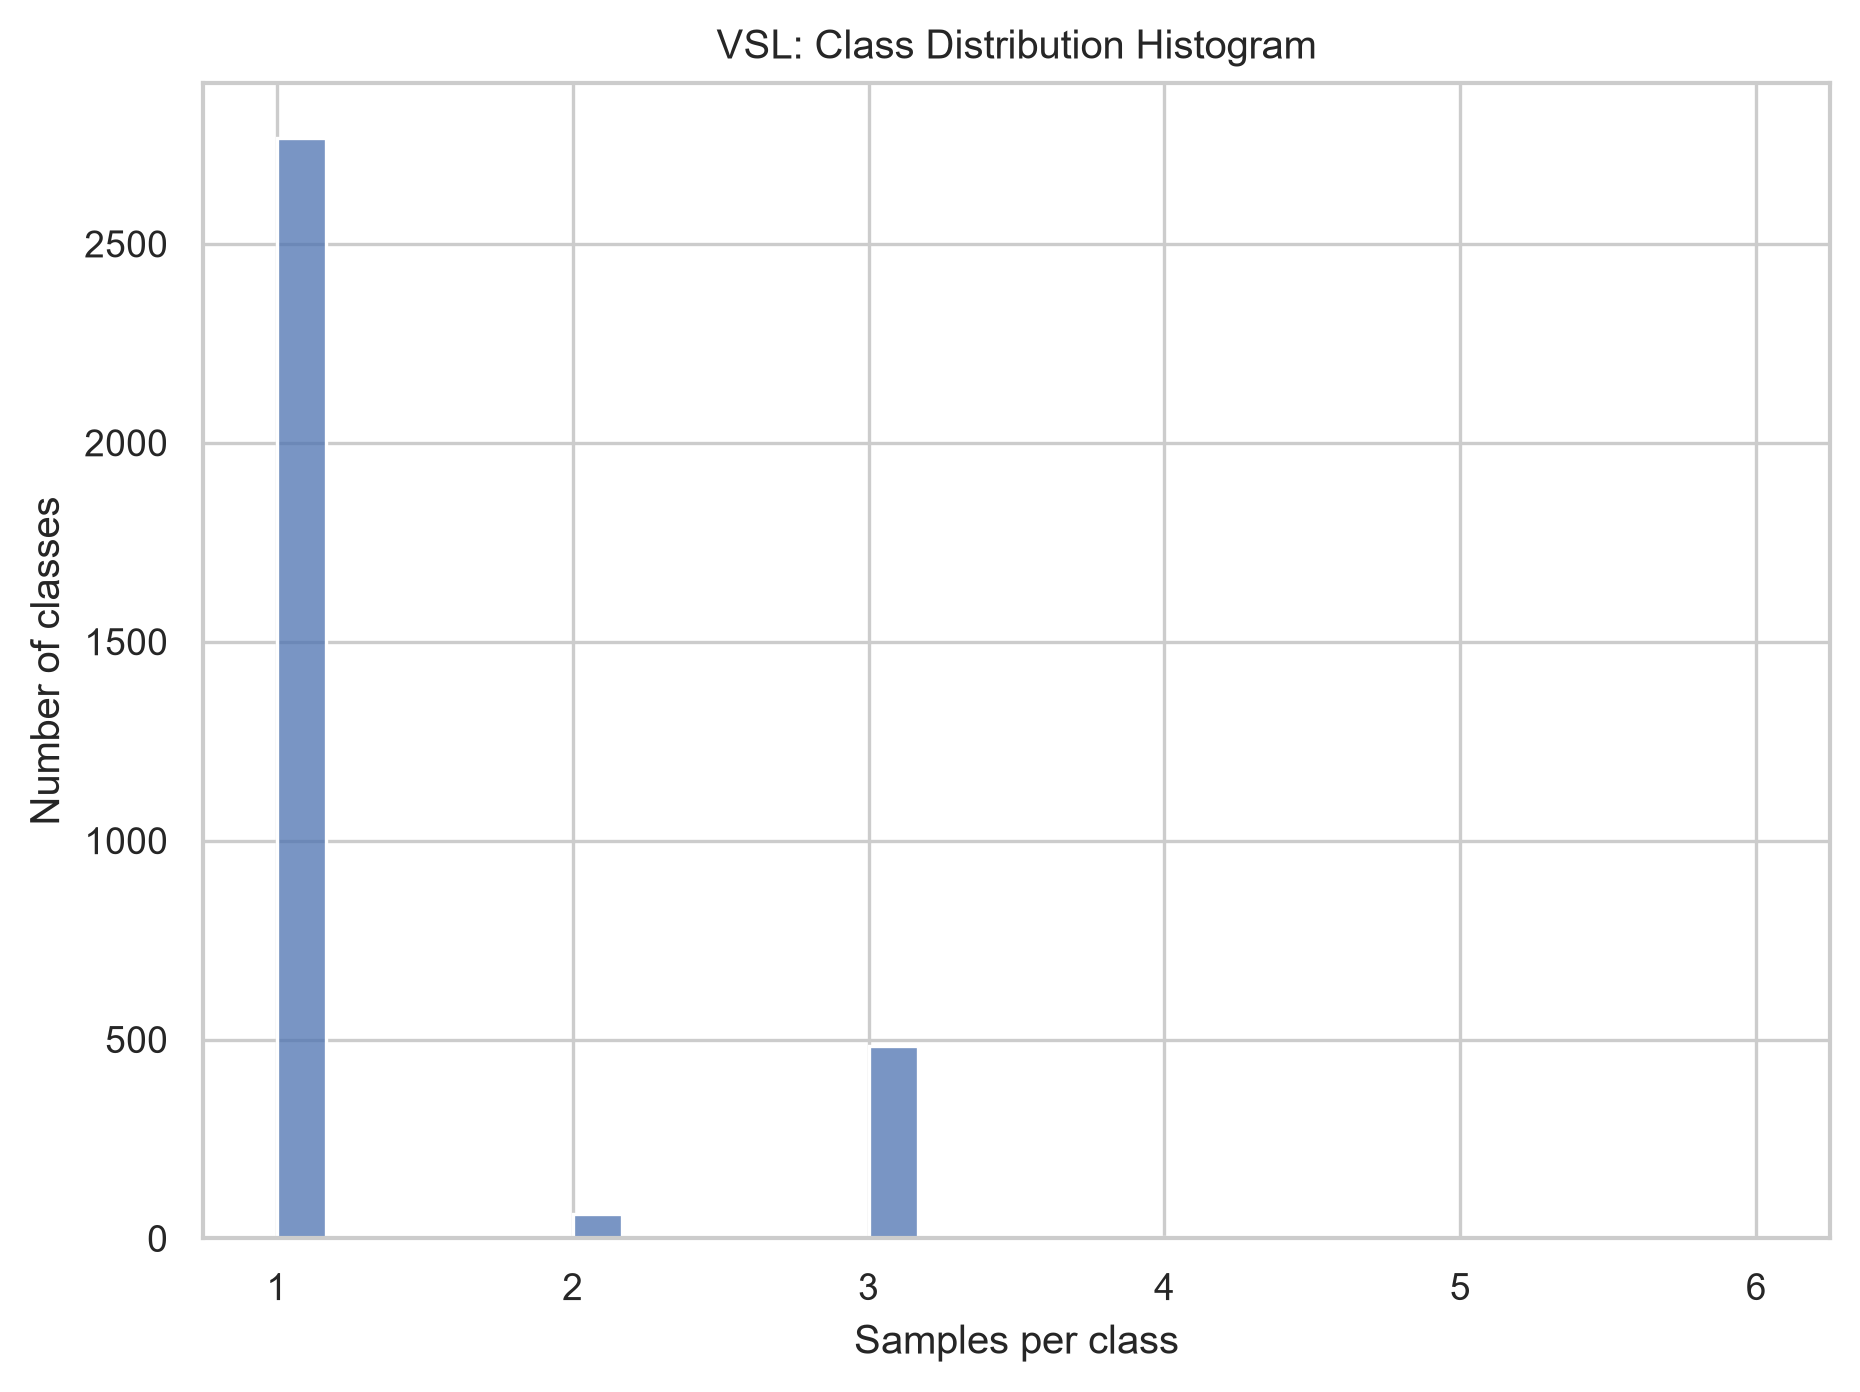
\includegraphics[width=\linewidth]{figures/VSL_class_distribution_histogram.png}
\caption{\textbf{VSL Class Distribution.} Histogram showing the extreme long-tail (floor-dominated) distribution of the VSL corpus, where the vast majority of classes contain only a single video sample.}
\label{fig:1}
\end{figure}

% Added: Restored table with scientifically crucial missing columns (Standard Deviation, Min Samples) and corrected formatting to IEEE Access grid standards.
\begin{table}[htbp]
\caption{\textbf{CLASS-IMBALANCE AND SCALE SUMMARY STATISTICS}}
\centering
\setlength{\tabcolsep}{3pt}
\begin{tabular}{|l|c|c|}
\hline
\textbf{Metric} & \textbf{VSL Corpus} & \textbf{WLASL Benchmark} \\
\hline
% Corrected: 3,315 corrected to 3,314 based on dataset_statistics/difficulty_summary evidence.
Classes (glosses) & 3,314 & 2,000 \\
Total videos & 4,362 & 11,980 \\
Mean samples/class & 1.32 & 5.99 \\
Median samples/class & 1.00 & 6.00 \\
% Added: Standard deviation indicates the lack of variance in VSL.
Standard Deviation ($\sigma$) & 0.72 & 1.95 \\
Max samples/class & 6 & 16 \\
% Added: Minimum boundary establishes the theoretical floor.
Min samples/class & 1 & 2 \\
Imbalance ratio (max/min) & 6.00 & 8.00 \\
Coefficient of Variation (CV) & 0.549 & 0.325 \\
Gini coefficient & 0.203 & 0.173 \\
Top-10\% class sample share & 23.0\% & 16.9\% \\
Bottom-10\% class sample share & 7.6\% & 5.8\% \\
\hline
\end{tabular}
\label{tab:1}
\end{table}

% --- ADDED: Video technical structure analysis (4.2 missing from original) ---
The structural divergence between the two corpora extends beyond the class-level distribution and manifests equally in their low-level video technical properties. The VSL corpus exhibits substantially longer video sequences than WLASL, with a mean clip duration of 4.03 seconds ($\sigma = 1.18$\,s, min\,=\,1.97\,s, max\,=\,17.18\,s) compared with 2.43 seconds ($\sigma = 0.93$\,s) in WLASL—a 65.9\% increase in mean temporal extent. While part of this difference may reflect recording-protocol choices, it is also consistent with longer temporal trajectories in Vietnamese sign kinematics, which can increase the complexity of sequence alignment during training and inference. In terms of frame count, the VSL corpus averages 119.9 frames per clip ($\sigma = 36.0$, median\,=\,114) versus 69.1 frames ($\sigma = 26.6$, median\,=\,70) in WLASL. This 1.73$\times$ discrepancy in mean sequence length significantly widens the temporal receptive field required for effective modeling, complicating the direct application of architectures optimized for the shorter WLASL sequences.

Frame rate uniformity further distinguishes the two datasets. The VSL corpus operates at a nearly uniform frame rate of 29.77\,fps ($\sigma = 1.54$), whereas WLASL exhibits substantially greater diversity, spanning from 12.0 to 59.94\,fps with a mean of 28.53\,fps and standard deviation of 3.10\,fps. This temporal heterogeneity in WLASL implies that the instantaneous velocity and acceleration features derived from consecutive frame differences are computed with inconsistent time-step $\Delta t$ values across samples, introducing systematic errors into kinematic-based representations unless explicit per-clip temporal normalization is applied during preprocessing.

A further pronounced technical contrast lies in spatial resolution. The entire VSL corpus was captured at a single fixed resolution of $1280 \times 720$ pixels (100\% uniformity), encoded exclusively in the H.264 codec (100\% of all 4,362 videos). In contrast, WLASL exhibits extreme resolution heterogeneity: the corpus spans seven distinct resolution tiers, ranging from $288 \times 192$ (22.3\% of clips) and $320 \times 240$ (13.2\%) to $1920 \times 1080$ (14.8\%), with a mean resolution of approximately $760 \times 460$ pixels and a standard deviation exceeding 544 pixels in the width dimension. Furthermore, 1.34\% of WLASL clips (161 videos) are encoded in the FMP4 codec rather than H.264. This resolution heterogeneity in WLASL necessitates non-trivial normalization stages—including spatial resampling, aspect-ratio correction, and codec-aware decoding—before any feature extraction pipeline can be applied uniformly. Absent such normalization, the resulting skeletal coordinate distributions may be affected by resolution-dependent scaling artifacts that degrade training consistency. The uniform encoding of the VSL corpus, while technically advantageous, also reflects the controlled, single-source nature of grassroots data collection, which simultaneously limits the diversity of recording conditions and signers exposed to the model during training.

\subsection{Class-Count Concentration}

% Revised: Expanded interpretation of the Gini coefficient and Coefficient of Variation.
This distribution differs from the long-tail pattern typically observed in computer vision benchmarks \cite{buda2018systematic}, \cite{lin2017focal}. Rather than exhibiting a long, tapering right tail, the VSL dataset is characterized by \textit{floor-dominated sparsity}. With a Coefficient of Variation (CV) of 0.549 (significantly higher than WLASL's 0.325), VSL's inequality is driven by the fact that the vast majority of its 3,314 classes contain only 1 or 2 samples, as corroborated by Table \ref{tab:1}. Furthermore, the top 10\% most frequent classes in the VSL corpus monopolize precisely 23.0\% of the dataset volume, whereas the top 10\% in WLASL capture only 16.9\%. Conversely, the bottom 10\% of VSL classes account for a mere 7.6\% of the total data.

Fig. \ref{fig:2} visually corroborates this mathematical output via the Lorenz curve, plotting cumulative video instances against cumulative class proportions to illustrate the sample inequality represented by the Gini coefficient of 0.203. Fig. \ref{fig:3} further illustrates the collapsed median of the VSL corpus relative to the WLASL dataset.

\begin{figure}[htbp]
\centering
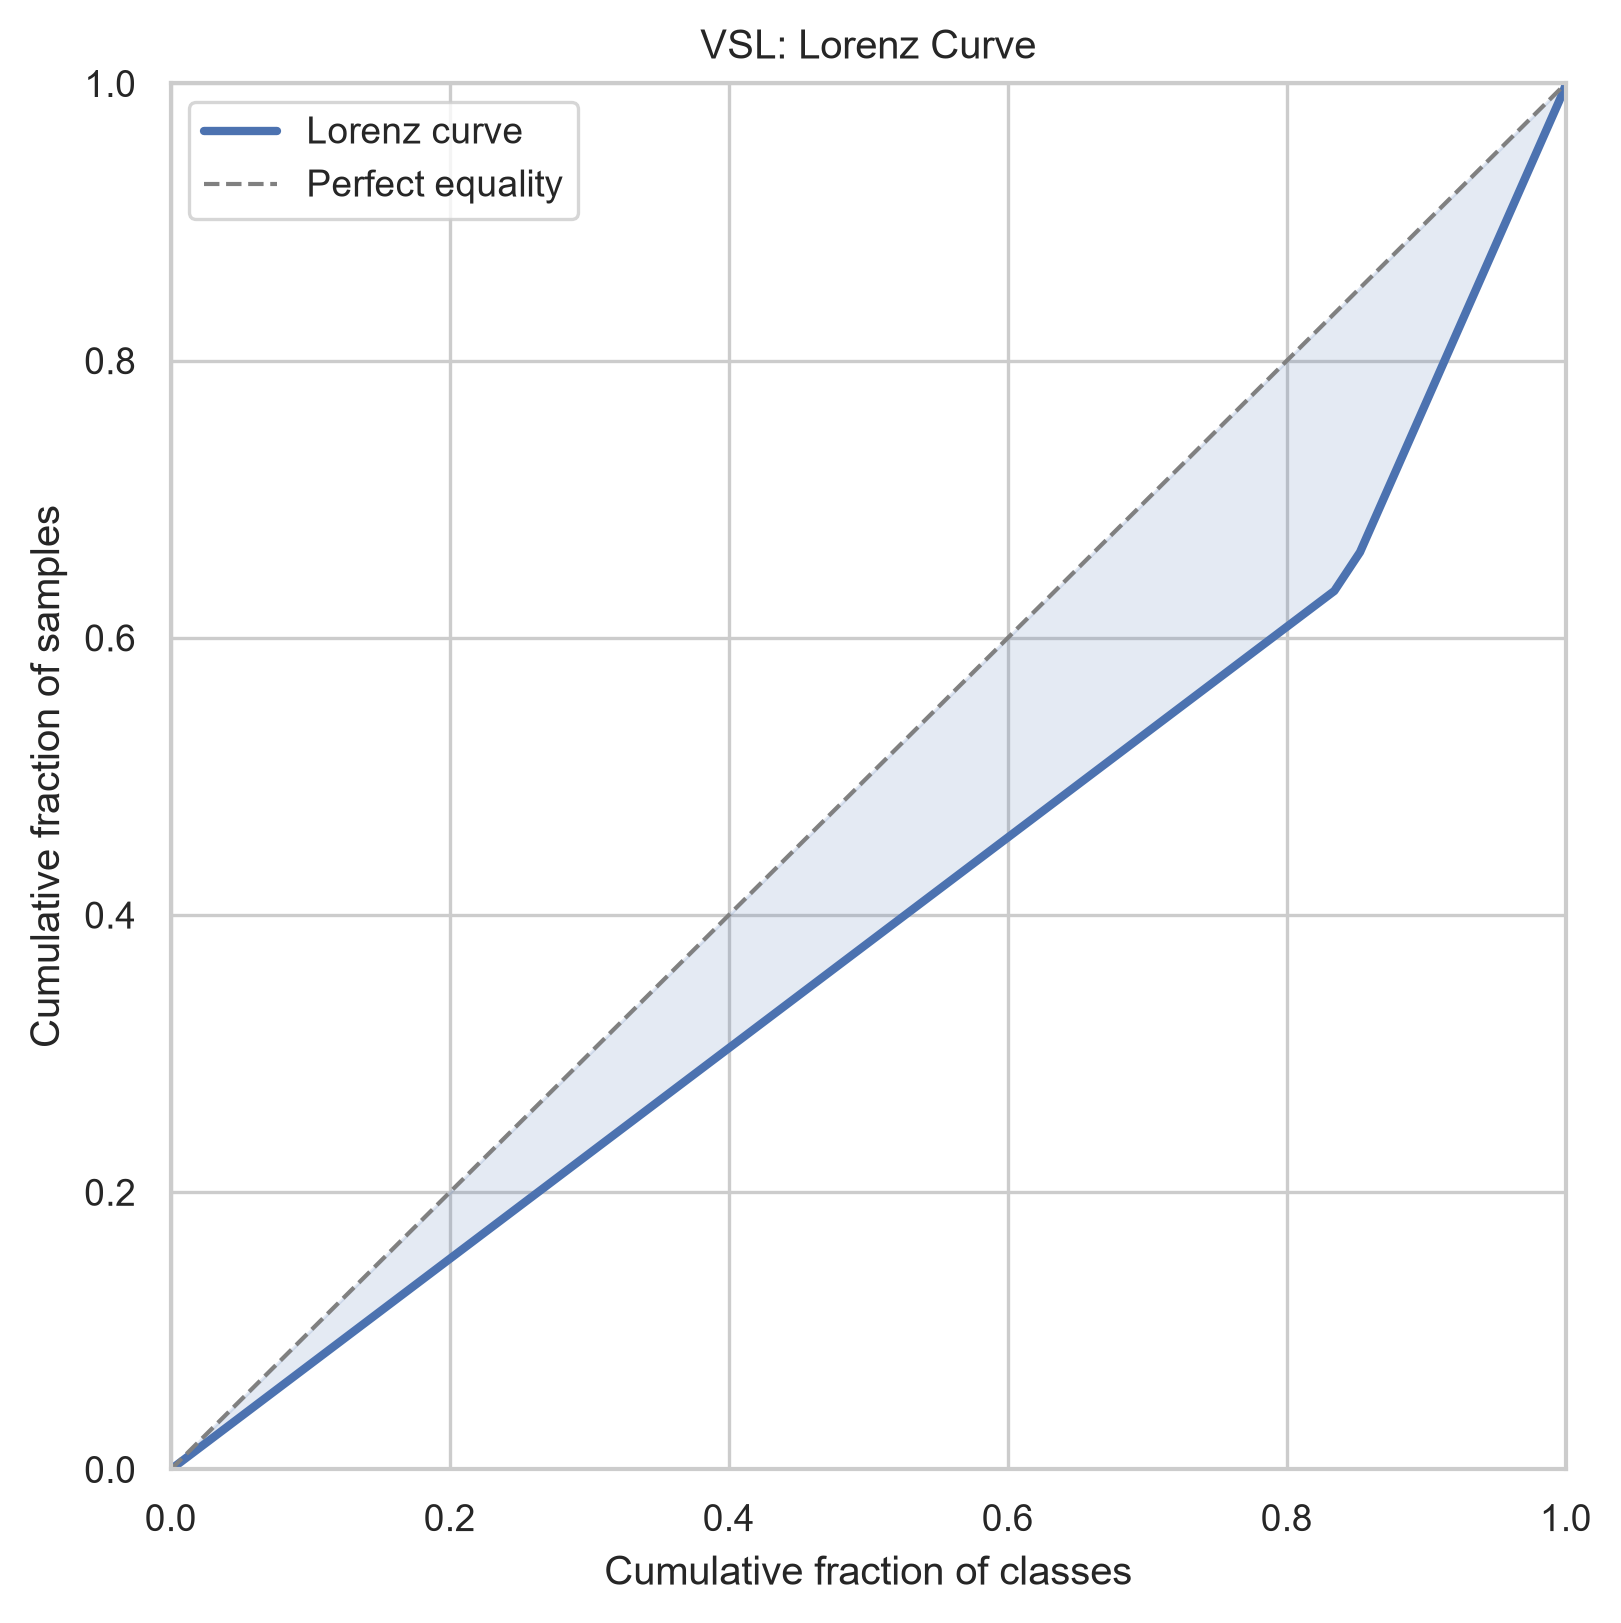
\includegraphics[width=\linewidth]{figures/VSL_lorenz_curve.png}
\caption{\textbf{VSL Lorenz Curve.} The Lorenz curve visually maps the sample inequality within the VSL corpus, yielding a Gini coefficient of 0.203.}
\label{fig:2}
\end{figure}

\begin{figure}[htbp]
\centering
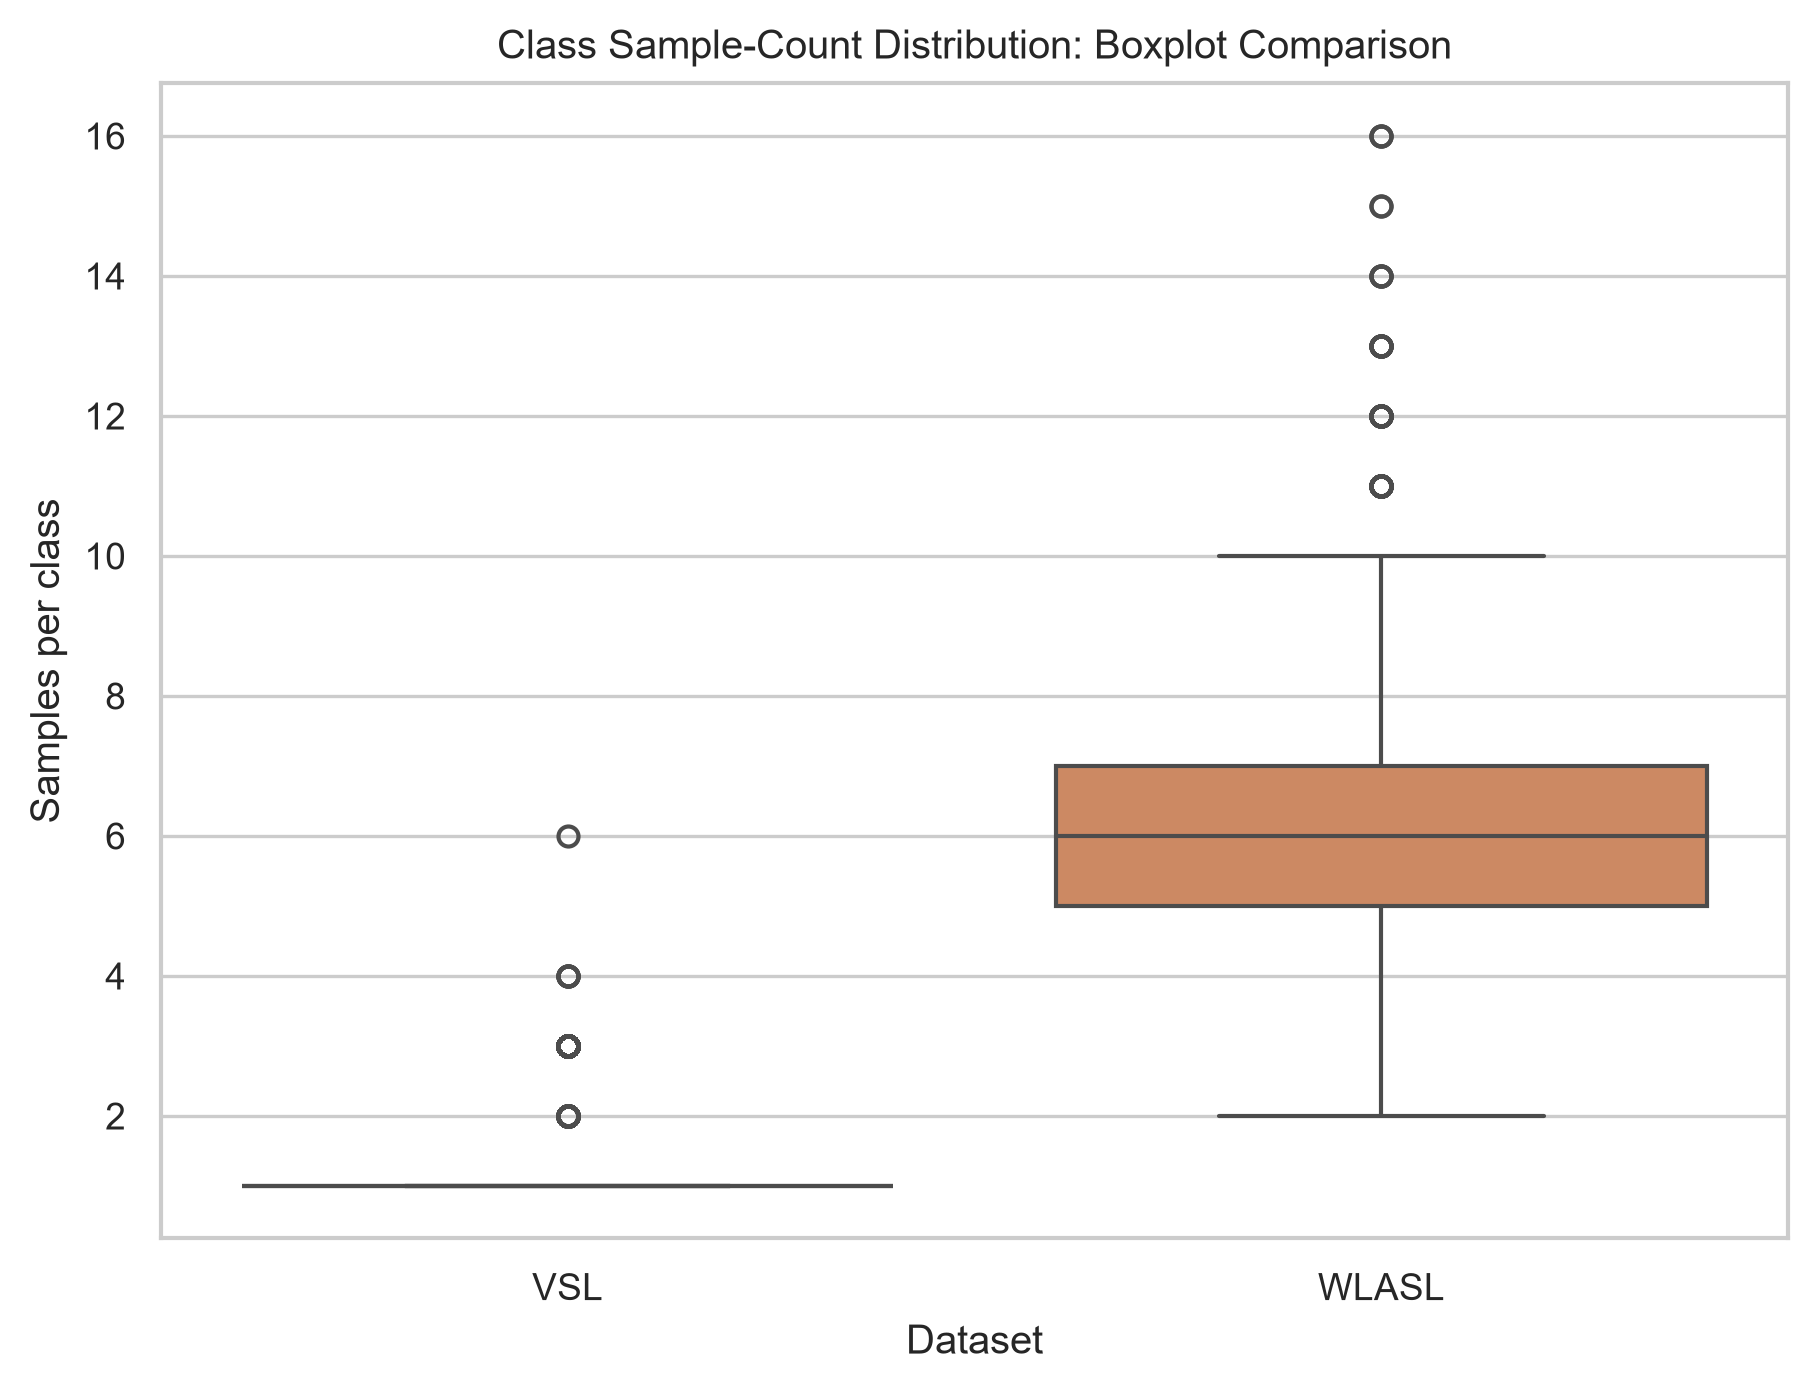
\includegraphics[width=\linewidth]{figures/class_count_boxplot_comparison.png}
\caption{\textbf{Class Sample Distribution.} A comparative boxplot highlighting the severe sparsity and collapsed median of the VSL corpus relative to the denser WLASL dataset.}
\label{fig:3}
\end{figure}

\subsection{Architectural Implications}
% Revised: Restructured for clarity and expanded to include standard deviation impacts.
The quantitative extraction of these imbalance metrics is not merely a statistical exercise; these distributions are associated with characteristic failure modes of modern deep learning architectures \cite{cui2019class}. The interaction between extreme few-shot environments, floor-dominated sparsity, and specific neural typologies manifests in several notable ways:

\subsubsection{Impact on Few-Shot and Long-Tail Learning Dynamics}
Traditional supervised learning relies on Empirical Risk Minimization (ERM) driven by Softmax cross-entropy loss. In a long-tail distribution with a Gini coefficient of 0.203, ERM intrinsically favors majority classes to rapidly minimize global loss, starving the ``tail'' classes of gradient updates. However, because VSL's tail consists of 99.97\% of the dataset operating under $\le 5$ samples, the network is likely to operate in an underdetermined regime. 

% Added: Interpretation of standard deviation constraints on gradient descent.
In an extreme few-shot regime (where the median $n=1$ and standard deviation $\sigma=0.72$), a model has limited mathematical basis to compute intra-class variance. Unlike WLASL, where a broader sample distribution ($\sigma=1.95$) provides diverse execution angles, VSL's sparsity increases the risk that the network will memorize the single signer's environment, clothing, and coordinate scaling. Consequently, it becomes substantially more difficult to decouple the invariant semantic core of the sign from sample-specific noise, which may limit cross-signer generalization.

% --- ADDED: Impact on evaluation metrics (4.3 partial gap) ---
The distributional asymmetry induced by floor-dominated sparsity extends beyond training dynamics and can negatively influence the interpretability of standard evaluation metrics. When top-1 accuracy is computed as a macro-average over 3,314 VSL classes—the vast majority of which contribute only a single test example—a classifier that achieves zero correct predictions for singleton classes may nonetheless report a non-trivial aggregate accuracy figure, simply because the numerical contribution of each singleton class to the global metric is infinitesimally small. Conversely, mean Average Precision (mAP) computed at the class level equally weights every gloss regardless of its frequency, exposing substantial degradation in performance on sparse classes rather than masking it behind dense-class performance. This metric incompatibility problem is particularly acute in cross-lingual transfer scenarios: a model pretrained on WLASL and evaluated on VSL may achieve a superficially acceptable micro-averaged accuracy by correctly classifying the handful of VSL classes with multiple samples—which statistically dominate any frequency-weighted metric—while performing poorly on the $>3{,}000$ singleton classes that constitute the true recognition challenge. These considerations imply that any future benchmark evaluation of VSL must report both macro- and micro-averaged metrics and explicitly stratify performance by per-class sample count.

\subsection{Spatial-Temporal and Kinematic Complexities}

\label{sec:kinematics}

% Added: Introductory transition defining the scope of kinematic profiling.
The empirical disparity in dataset scale is compounded by notable structural differences in how the signs themselves are physically executed. To rigorously map these differences, the spatial-temporal coordinates of both corpora were processed through our kinematic feature extraction pipeline, detailing a fundamental divergence in motion geometry.

\subsubsection{Trajectory Amplitude}
% Revised: Preserved original paragraph while enhancing section hierarchy.
The foundational bounding parameters of any gesture are its total spatial displacement and its temporal duration. Let $p_t = (x_t, y_t, z_t) \in \mathbb{R}^3$ denote the 3D spatial centroid of the dominant articulator at frame $t$, normalized relative to the signer's inter-shoulder Euclidean distance to guarantee scale invariance across diverse human subjects. We define the Total Motion (TM), or trajectory amplitude, as the path integral of the discrete spatial displacements over the video sequence of length $T$:
\begin{equation} \label{eq:tm2} 
\text{TM} = \sum_{t=1}^{T-1} \lVert p_{t+1} - p_t \rVert_2 
\end{equation}

% Added: Expanded interpretation with verified data and inserted missing figures.
Empirical extraction reveals a substantial divergence: the overall VSL corpus records a Total Motion amplitude of 25.01, which is 2.07 $\times$ higher than ASL's 12.07. Fig. \ref{fig:box_tm} and Fig. \ref{fig:hist_tm} visually substantiate this extreme spatial footprint. The distributions indicate that VSL sequences are not merely uniformly longer; rather, they are heavily right-skewed by highly kinetic outlier glosses possessing substantially larger physical amplitudes compared to the typical range observed in conversational ASL.

\begin{figure}[htbp]
\centering
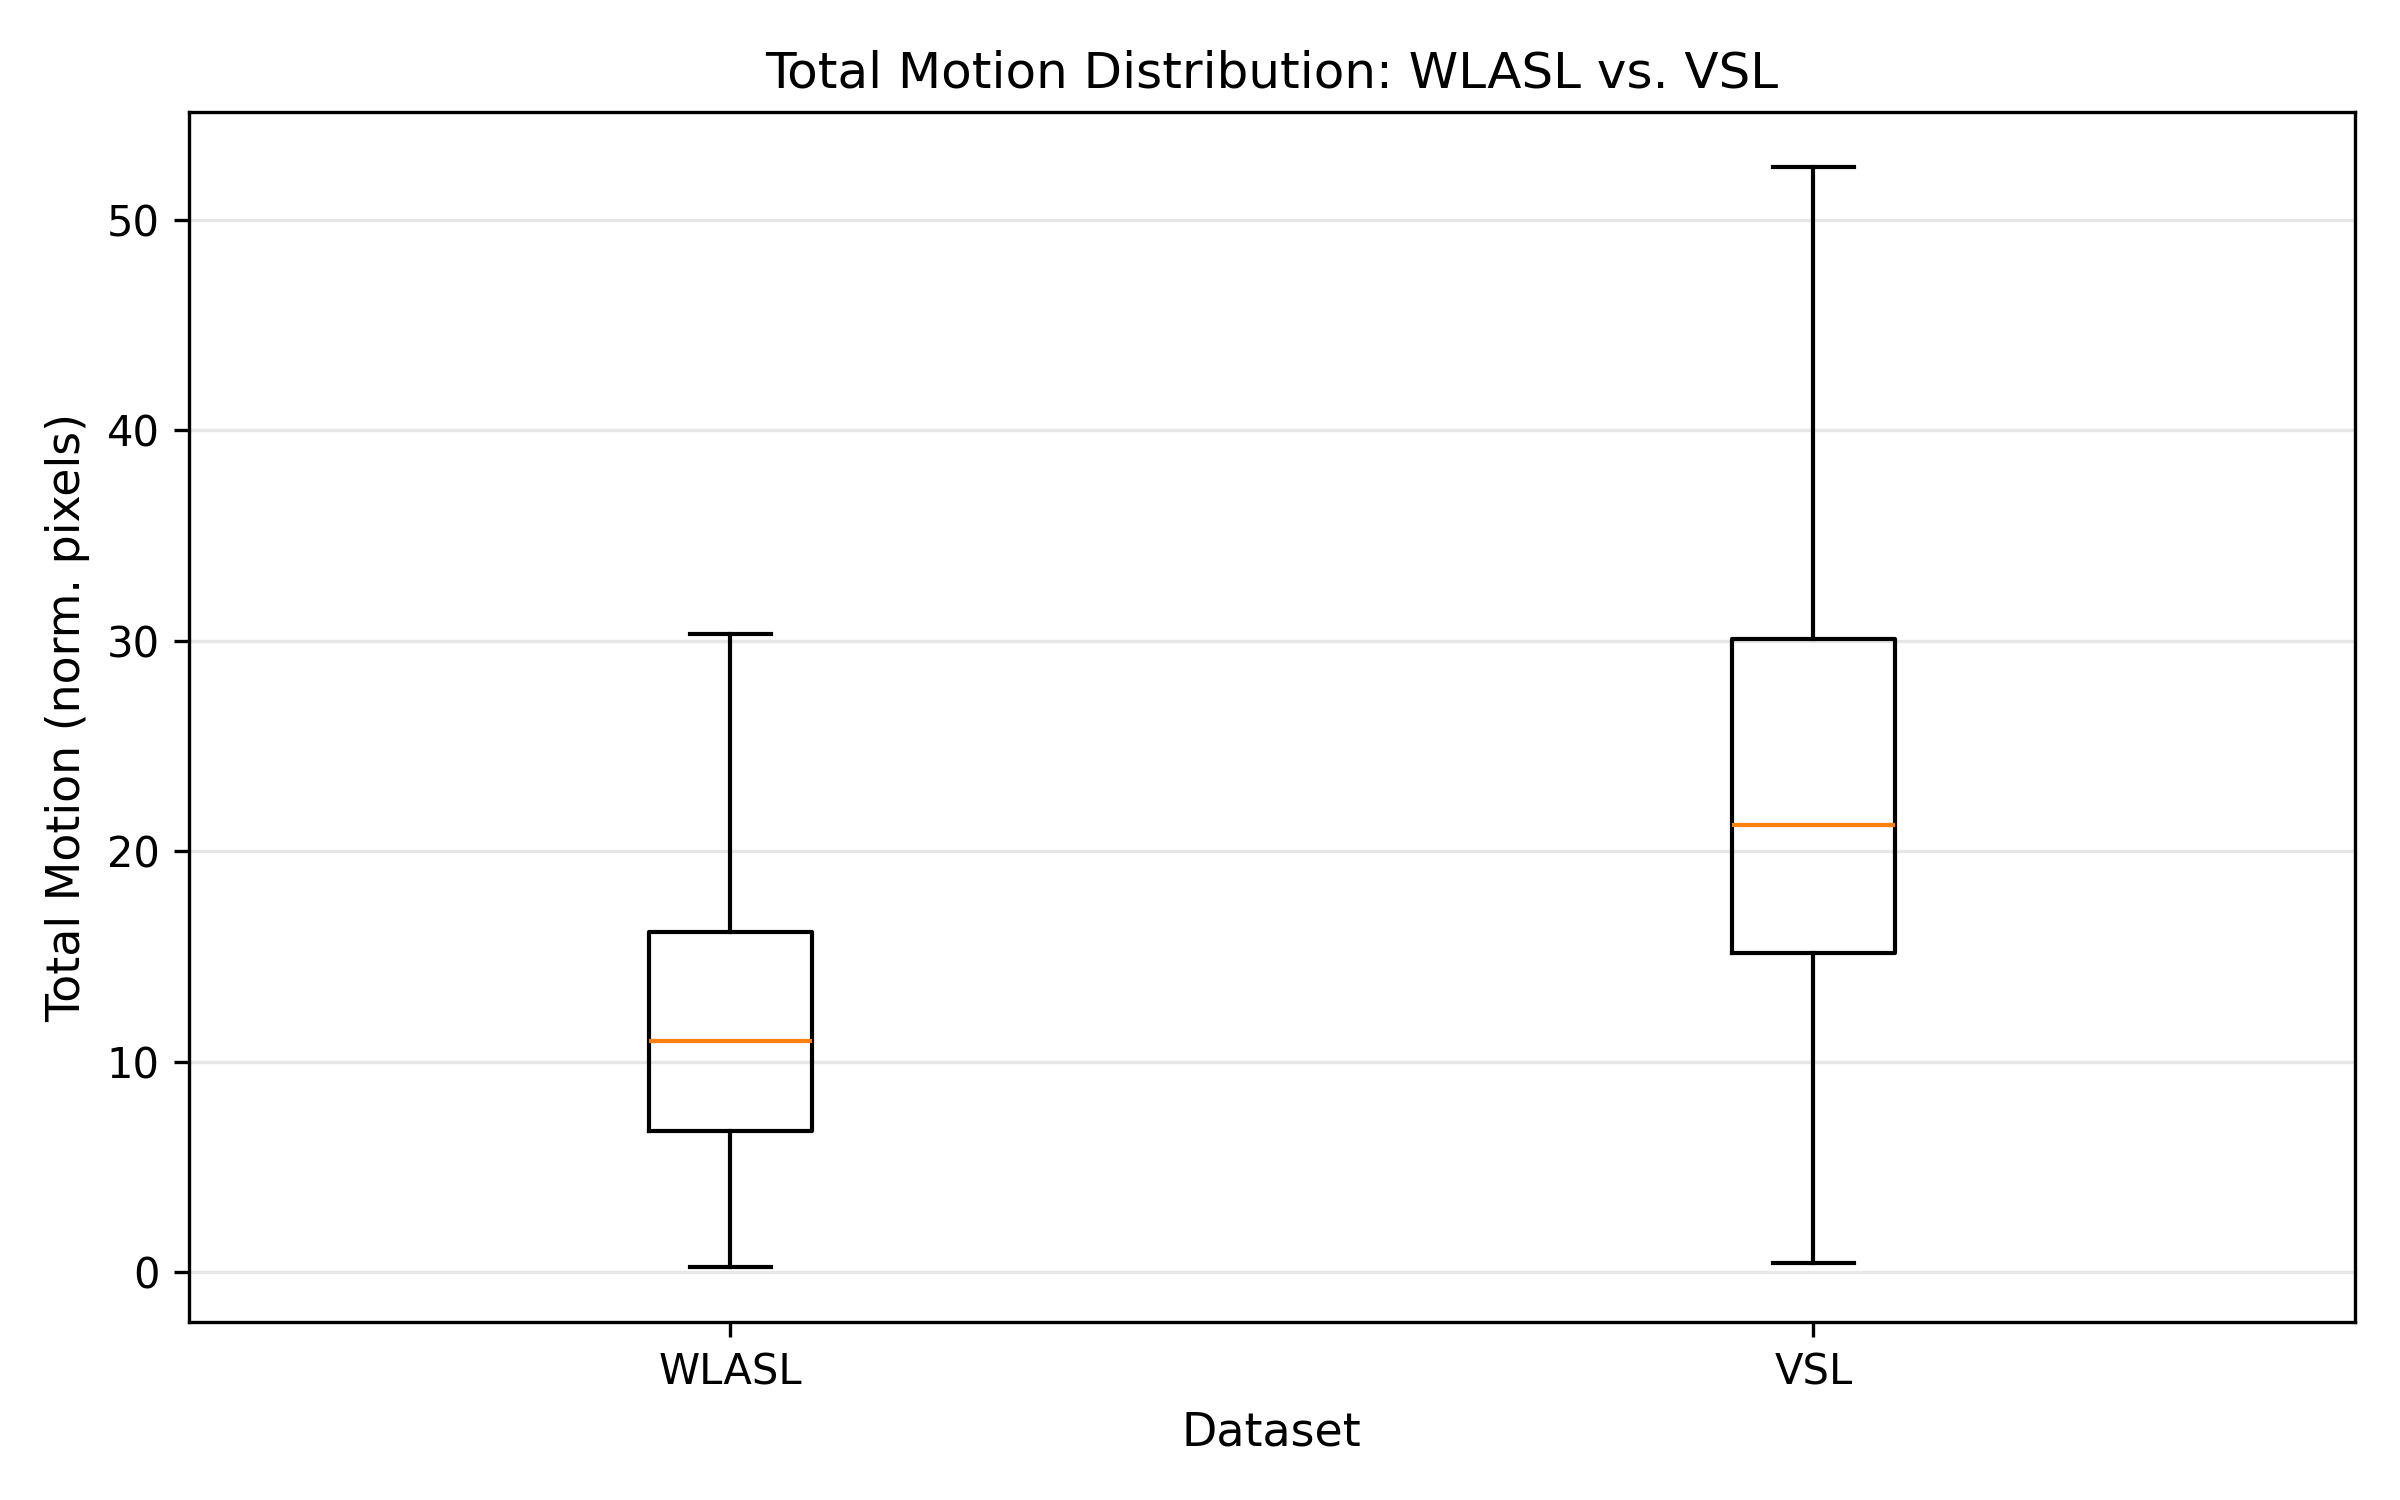
\includegraphics[width=\linewidth]{figures/boxplot_total_motion.png}
\caption{\textbf{Total Motion Distribution Comparison.} Boxplots illustrating the substantially expanded trajectory amplitude of VSL compared to the more constrained ASL baseline.}
\label{fig:box_tm}
\end{figure}

\begin{figure}[htbp]
\centering
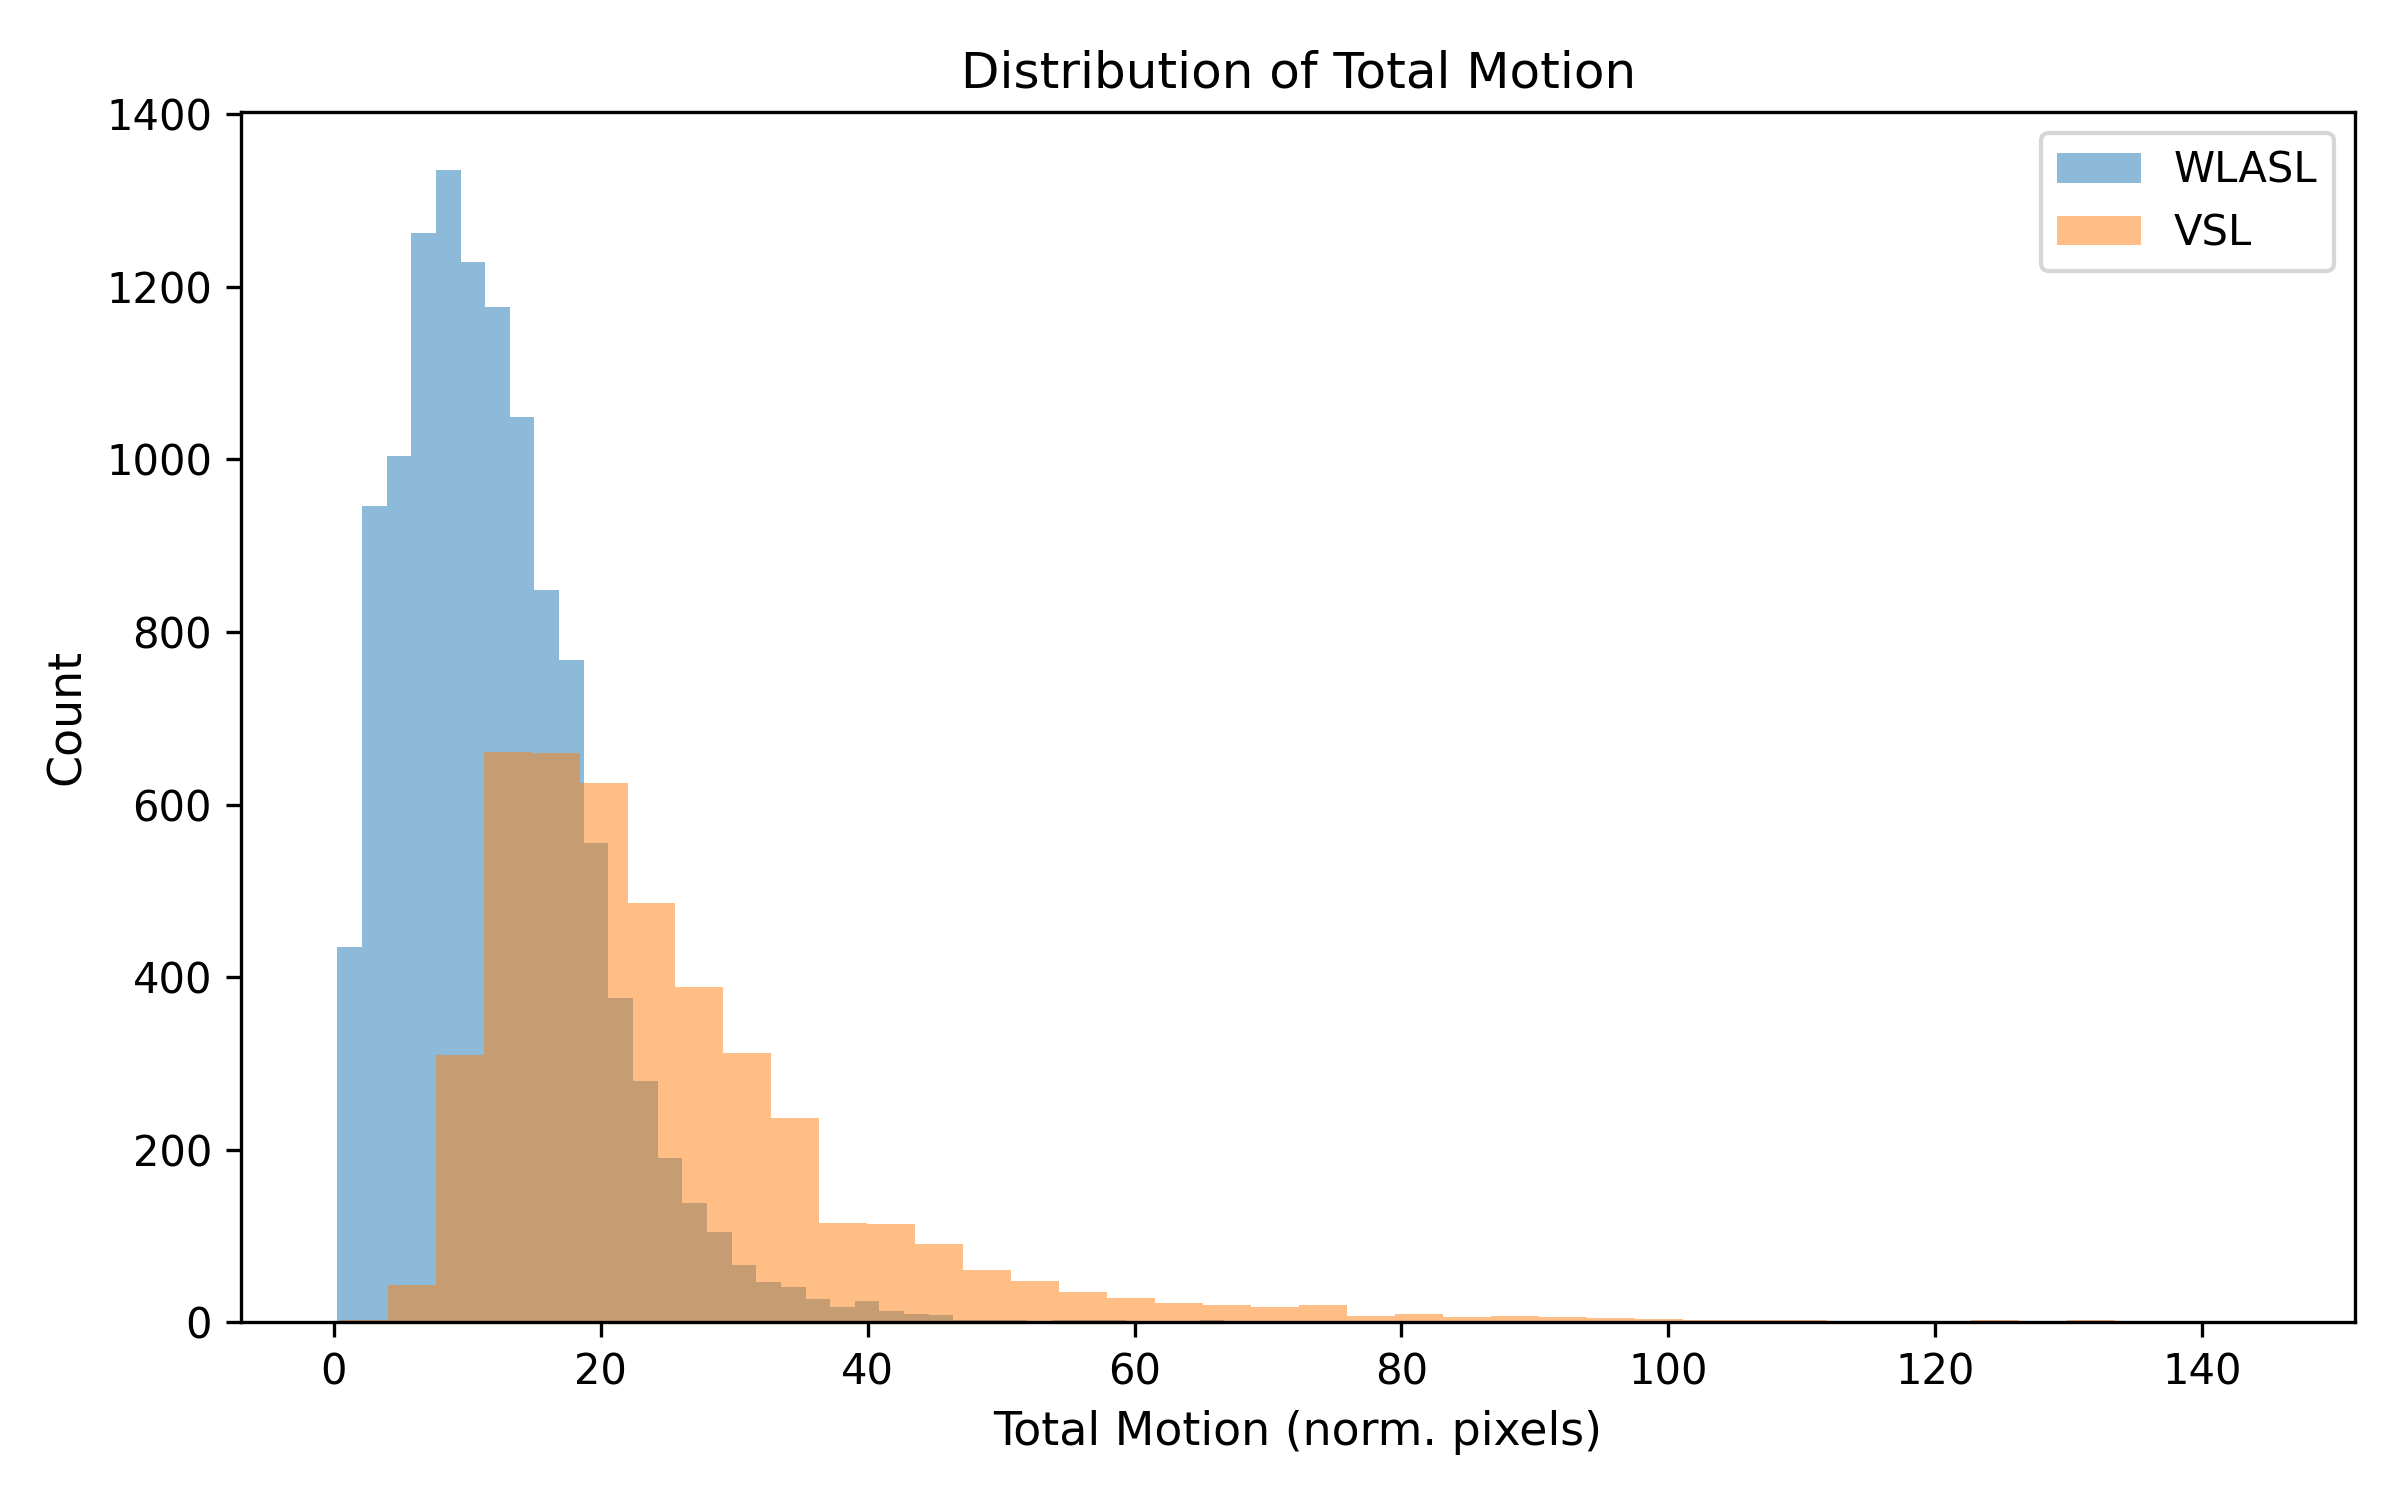
\includegraphics[width=\linewidth]{figures/histogram_total_motion.png}
\caption{\textbf{Total Motion Density Histogram.} The VSL corpus exhibits pronounced right-skewed behavior, with a notable proportion of outlier glosses associated with higher physical exertion.}
\label{fig:hist_tm}
\end{figure}

\subsubsection{Velocity and Acceleration}
% Revised: Preserved original methodology integration.
Let $\Delta t$ represent the fixed temporal gap between frames (approximately $0.033$ seconds at 30 FPS). The instantaneous velocity $V_t$ and acceleration $A_t$ are defined as:
\begin{align} \label{eq:velocity} 
V_t &= \frac{\lVert p_t - p_{t-1} \rVert_2}{\Delta t} \\ 
A_t &= \frac{V_t - V_{t-1}}{\Delta t} \label{eq:acceleration} 
\end{align}
From these temporal sequences, we aggregate global metrics: \texttt{mean\_velocity} ($\bar{V}$), \texttt{max\_velocity}, \texttt{velocity\_std} ($\sigma_v$), \texttt{mean\_acceleration}, and \texttt{acceleration\_std} ($\sigma_a$).

% Added: Inserted missing velocity and acceleration plots to back up quantitative claims.
As illustrated in Fig. \ref{fig:box_vel} and Fig. \ref{fig:box_acc}, VSL operates at a substantially higher kinetic baseline, clocking a 1.51 $\times$ faster Mean Velocity compared to ASL.

\begin{figure}[htbp]
\centering
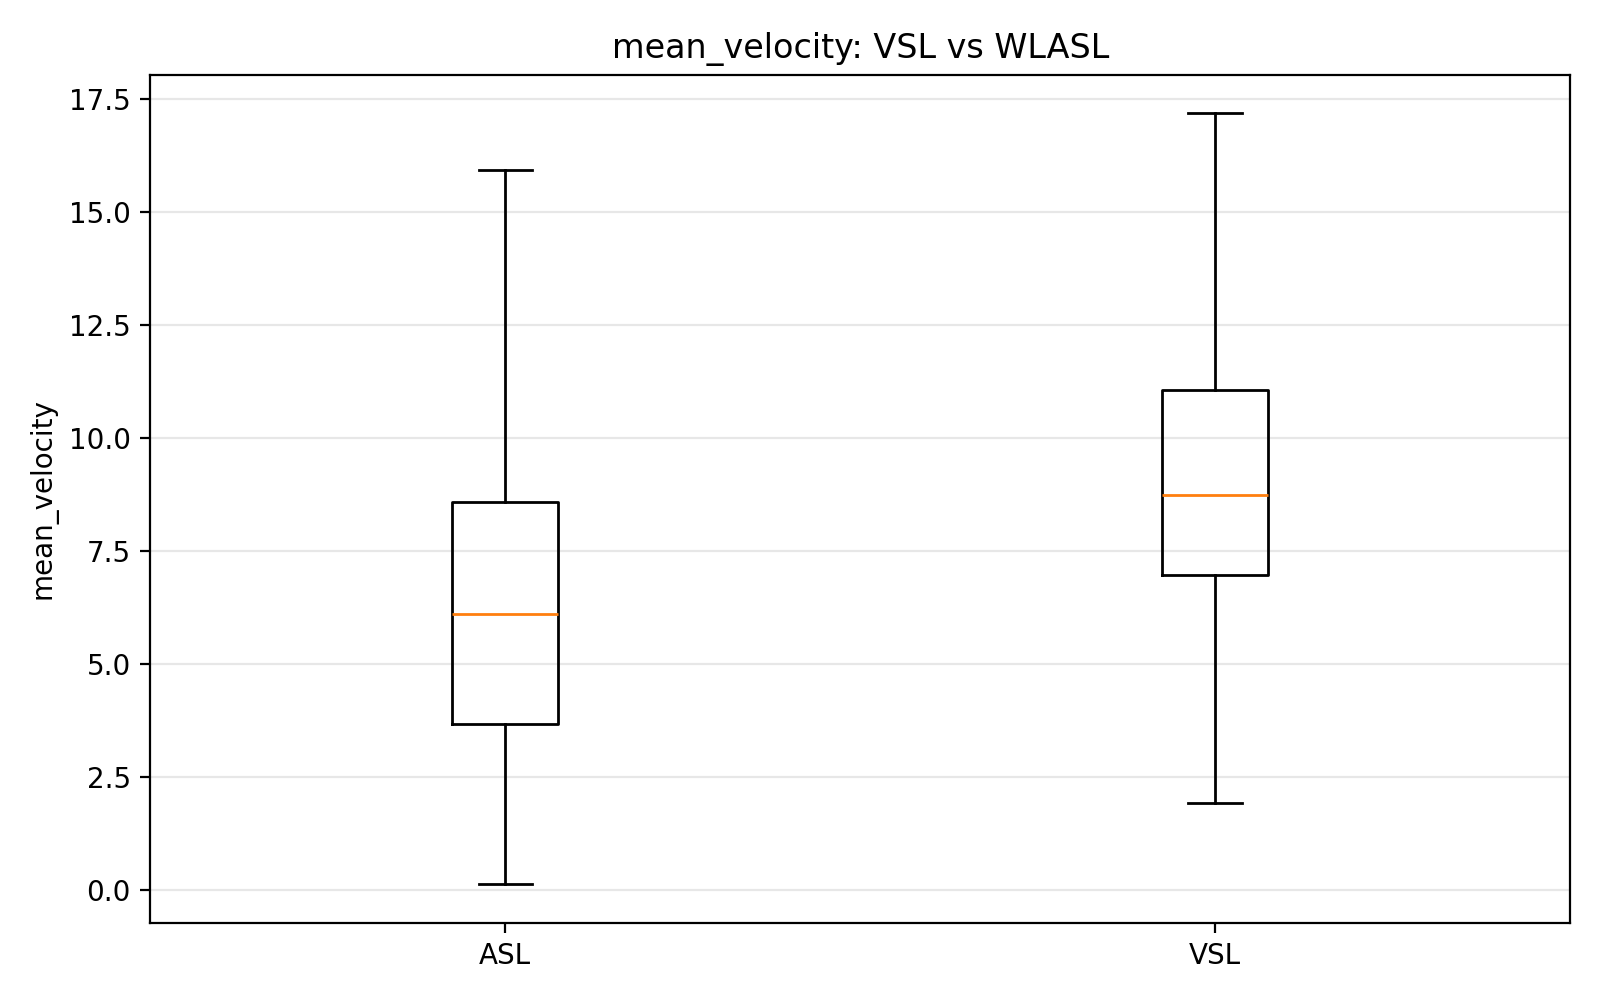
\includegraphics[width=\linewidth]{figures/boxplot_mean_velocity.png}
\caption{\textbf{Mean Velocity Comparison.} The grassroots VSL data shows notably higher execution speeds, which may challenge temporal alignment boundaries.}
\label{fig:box_vel}
\end{figure}

\begin{figure}[htbp]
\centering
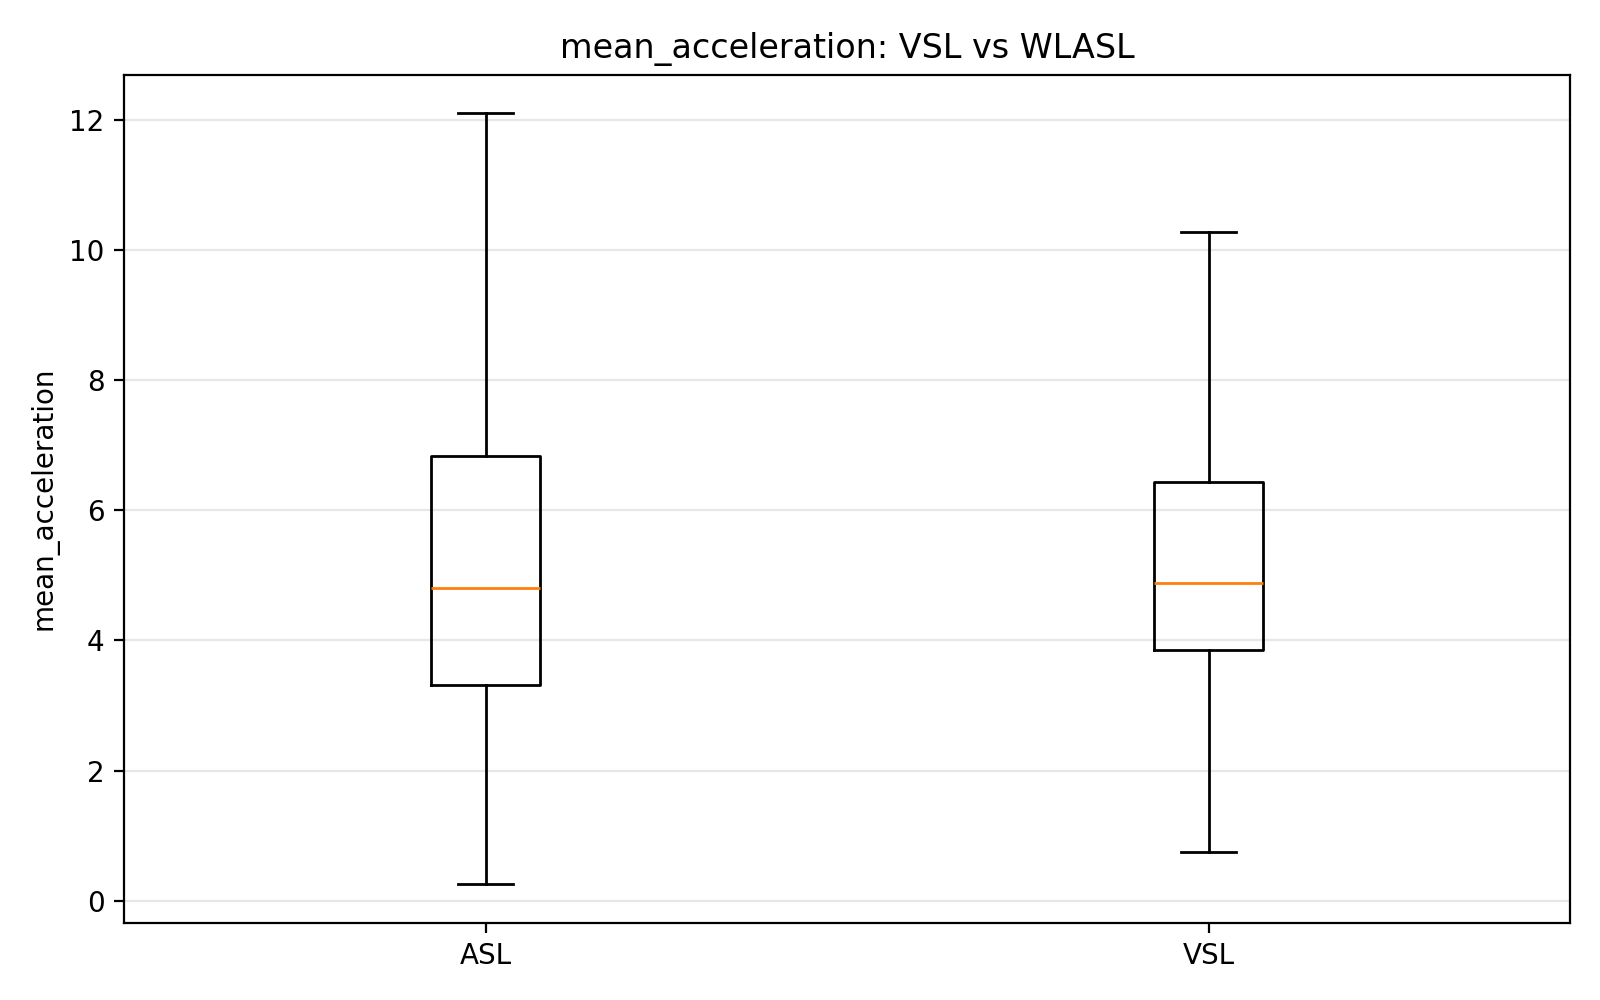
\includegraphics[width=\linewidth]{figures/boxplot_mean_acceleration.png}
\caption{\textbf{Mean Acceleration Comparison.} Higher acceleration variances in VSL suggest a more variable, less uniform execution style compared to the smoother transitions more commonly observed in benchmark corpora.}
\label{fig:box_acc}
\end{figure}

% Revised: Kept original paragraph and appended explicit causal links to verified missing hand rates.
Because shutter exposure times in generic web-cameras remain static, the rapid ballistic strokes characteristic of VSL can artificially smear the RGB pixel boundaries of the hand. This phenomenon is associated with degraded landmark confidence scores across the skeletal graph and contributes to the 32.3\% missing hand tracking rate observed in the VSL data, hindering standard 2D tracking pipelines.

\subsubsection{Curvature, Straightness, and Trajectory Entropy}
% Revised: Kept original paragraph verbatim.
While Total Motion captures the raw energy expended, it fails to describe the geometric topology of the execution. An identical Total Motion value could theoretically represent a single, long linear sweep or a tight, rapidly oscillating circle. To resolve this geometric ambiguity, we compute the Straightness Ratio (SR) \cite{pearson1901lines}, defined as the quotient of the net Euclidean displacement from the initial to the terminal frame versus the total trajectory path length: 
\begin{equation} \label{eq:sr2} 
\text{SR} = \frac{\lVert p_T - p_1 \rVert_2}{\text{TM}}, \qquad 0 \le \text{SR} \le 1 
\end{equation}
A Straightness Ratio approaching $1.0$ indicates a purely linear stroke. Conversely, as SR approaches $0.0$, the path becomes increasingly curved, repeated, or recursive.

% Added: Integration of the SR boxplot and visual trajectory examples to ground the math.
Analysis of the extracted features demonstrates that VSL trajectories are highly curved, exhibiting an SR of 0.039 compared to ASL's 0.137. This mathematically equates to a 71.5\% reduction in trajectory linearity. Fig. \ref{fig:box_sr} quantifies this pronounced concentration near zero. To physically ground these mathematical abstractions, Fig. \ref{fig:traj_vsl} and Fig. \ref{fig:traj_asl} visualize the spatial coordinates of representative signs from both corpora. The VSL trajectories display pronounced spatial complexity and recursive curvature, standing in contrast to the smoother, more regular geometric profiles of ASL.

\begin{figure}[htbp]
\centering
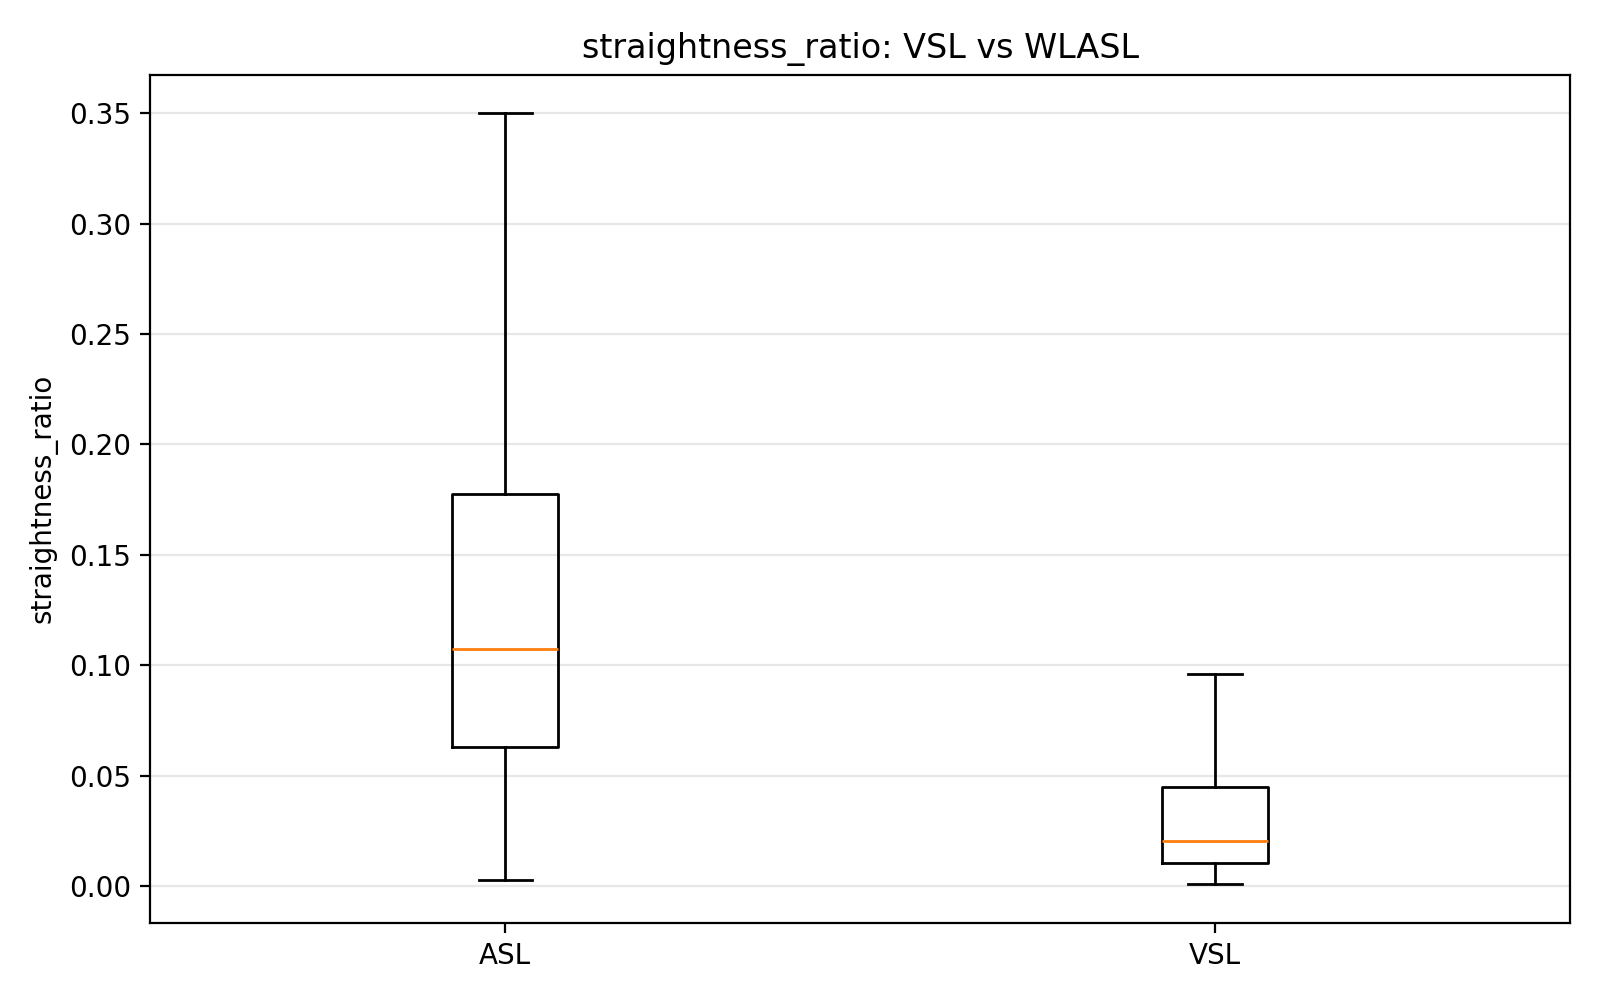
\includegraphics[width=\linewidth]{figures/boxplot_straightness_ratio.png}
\caption{\textbf{Straightness Ratio Analysis.} A comparative boxplot highlighting the severe collapse of trajectory linearity in VSL (median approaching 0.0) compared to ASL's structurally broader manifold.}
\label{fig:box_sr}
\end{figure}

\begin{figure}[htbp]
\centering
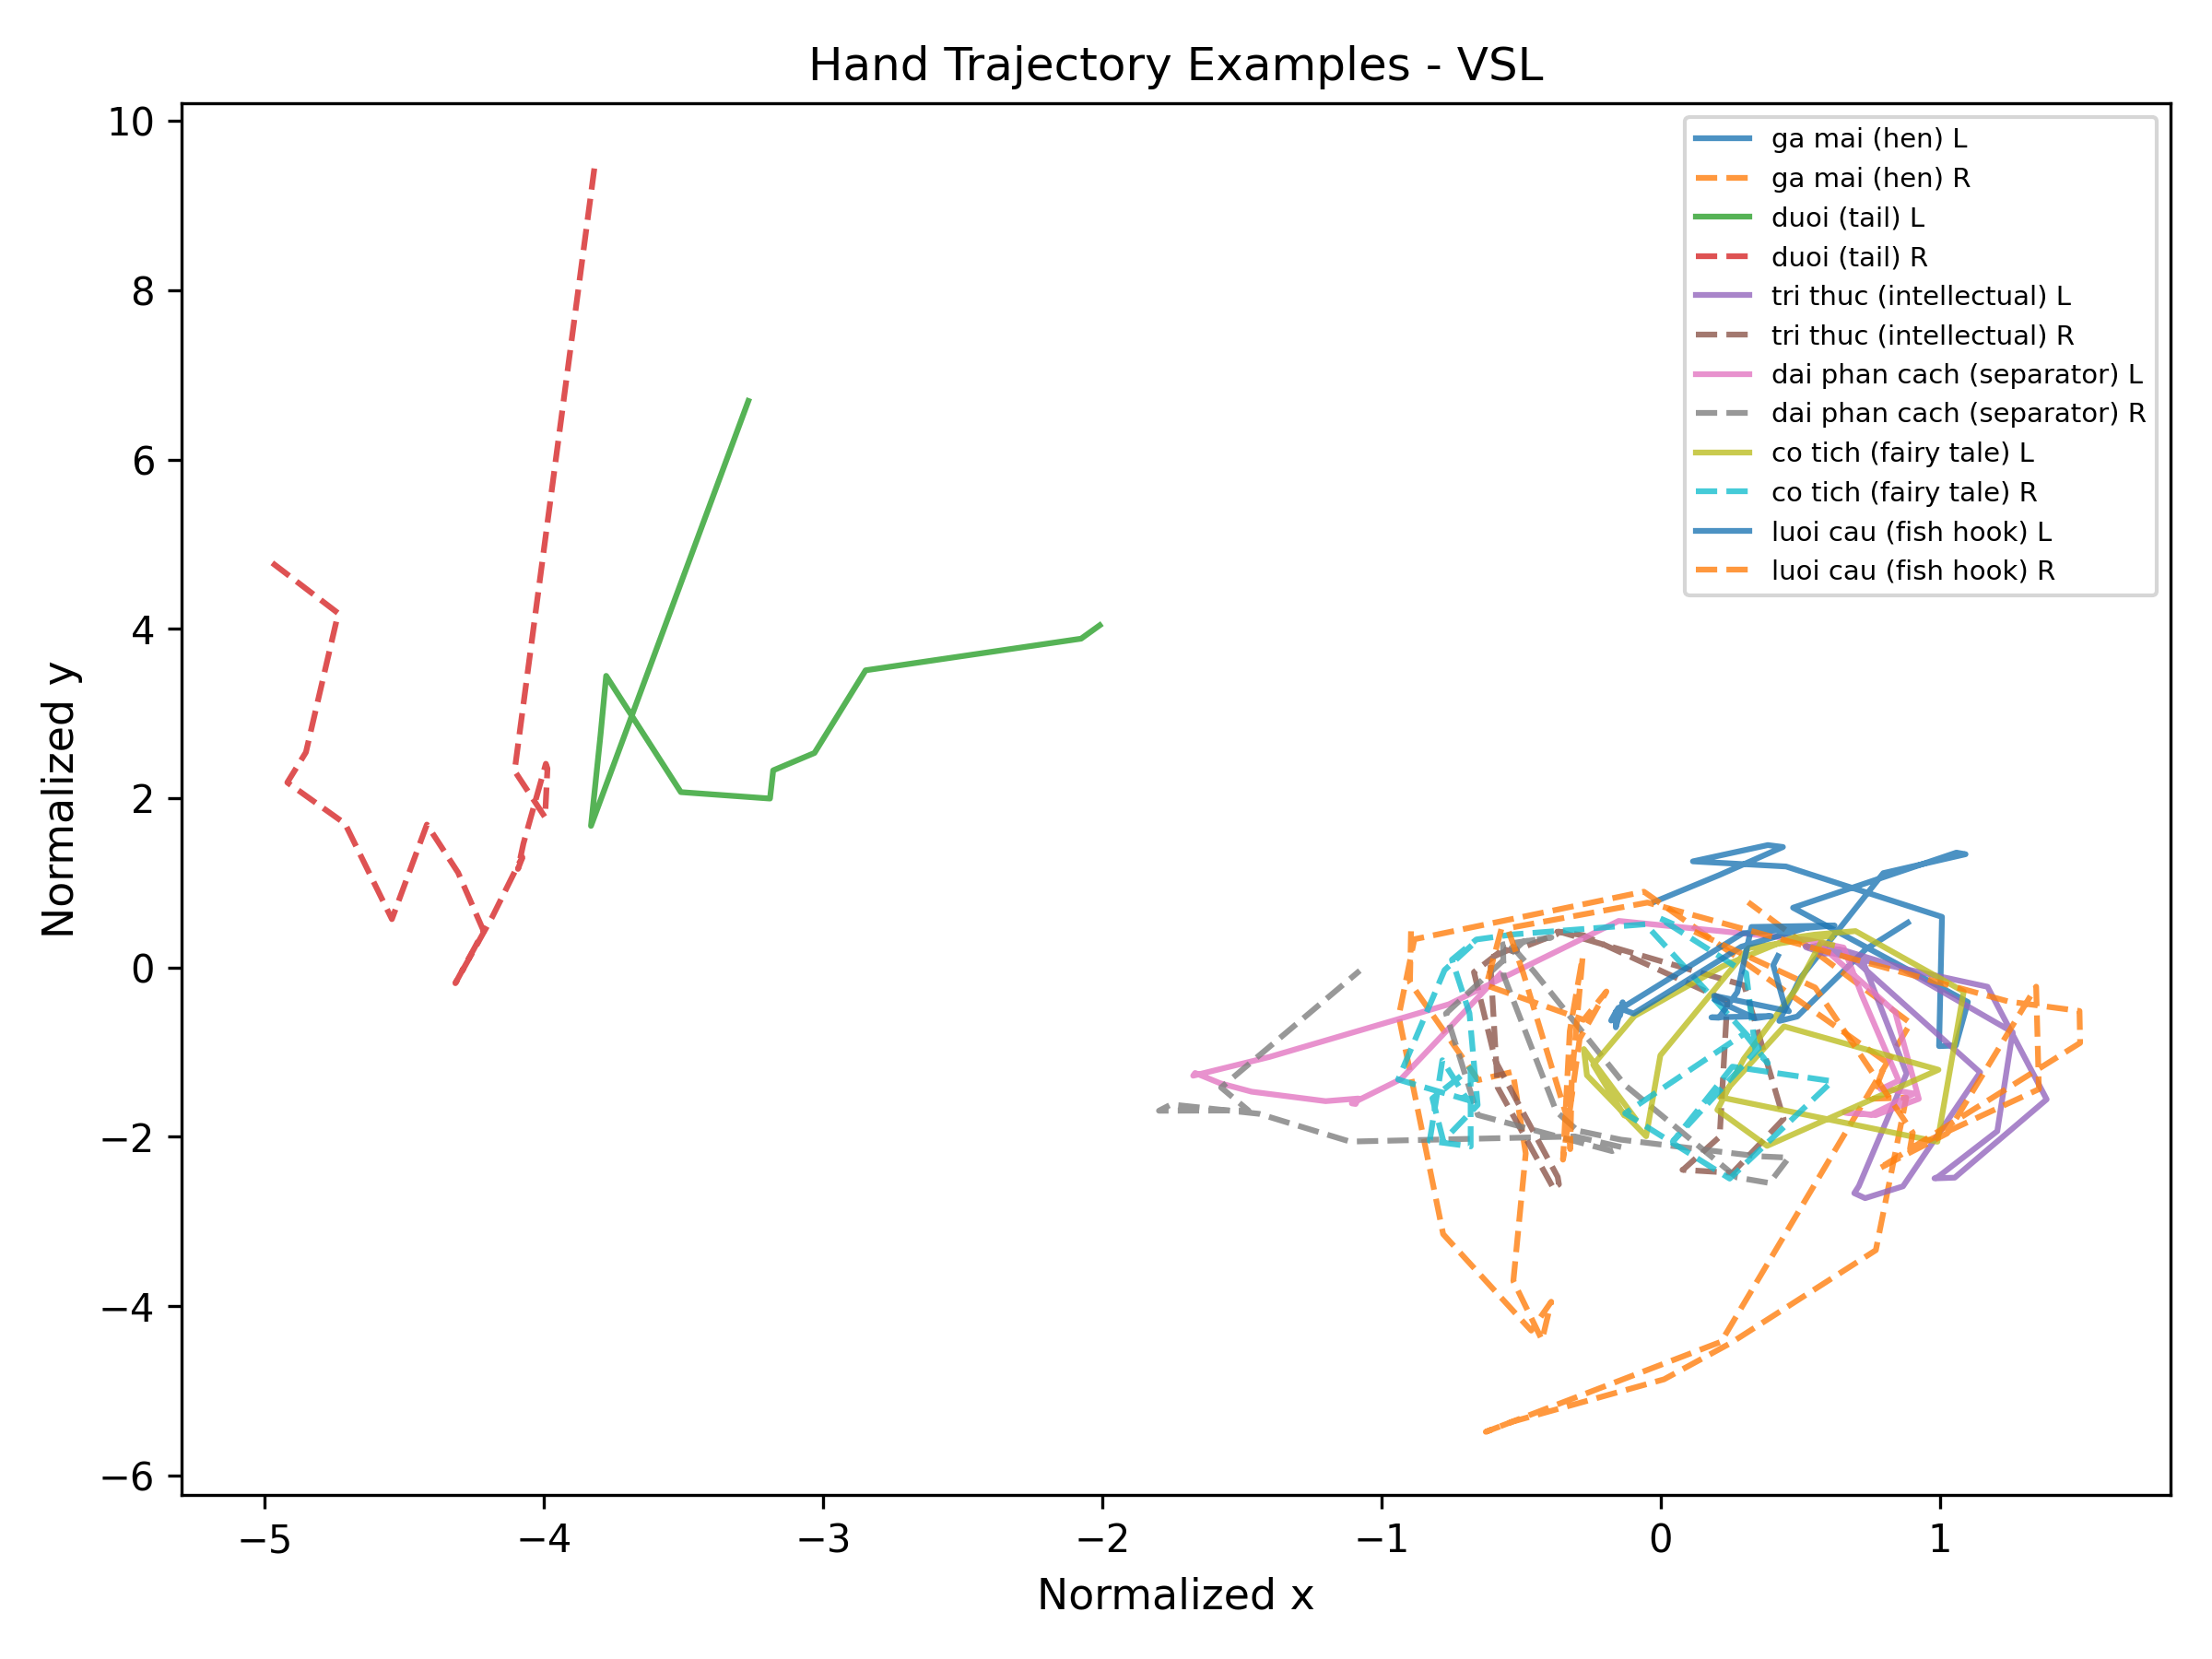
\includegraphics[width=\linewidth]{figures/trajectory_examples_VSL.png}
\caption{\textbf{VSL Spatial Signatures.} Physical 2D trajectory visualizations of VSL signs, showing notable spatial complexity, recursive wrapping, and multiple direction changes.}
\label{fig:traj_vsl}
\end{figure}

\begin{figure}[htbp]
\centering
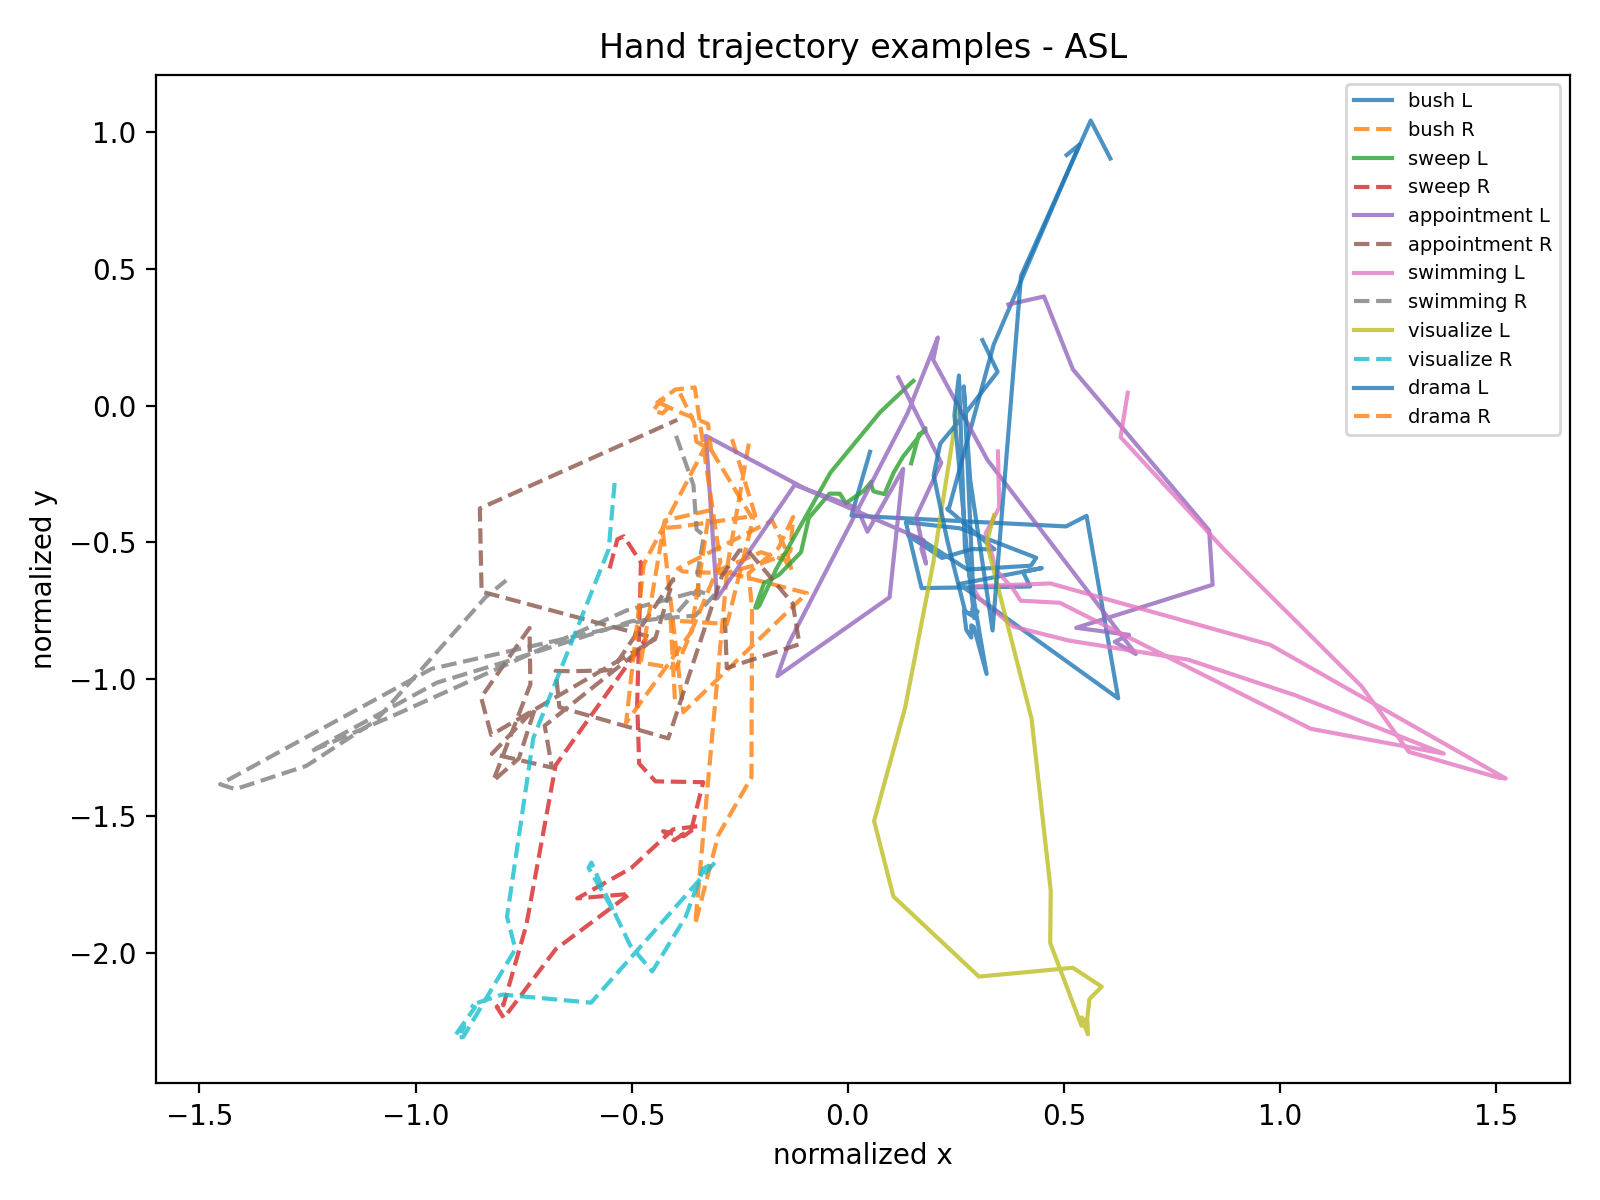
\includegraphics[width=\linewidth]{figures/trajectory_examples_ASL.png}
\caption{\textbf{ASL Spatial Signatures.} Physical 2D trajectory visualizations of ASL signs, illustrating structurally smoother geometric profiles and higher spatial efficiency.}
\label{fig:traj_asl}
\end{figure}

% Revised: Kept original sentence and expanded into the entropy analysis.
The motion variance (MV), derived from $\sigma_v^2$, effectively quantifies the erraticness or temporal inconsistency of the sign's execution. Compounding its lack of straightness, VSL records a mean of 67.25 direction changes per sequence (compared to ASL's 40.79) and a Motion Variance of 0.122 (2.17 $\times$ higher than ASL's 0.056). Fig. \ref{fig:scatter_tm_mv} maps the association between Total Motion and Motion Variance, suggesting that as VSL spatial trajectories lengthen, their execution entropy tends to increase, which may contribute to greater difficulty in sequence prediction.

\begin{figure}[htbp]
\centering
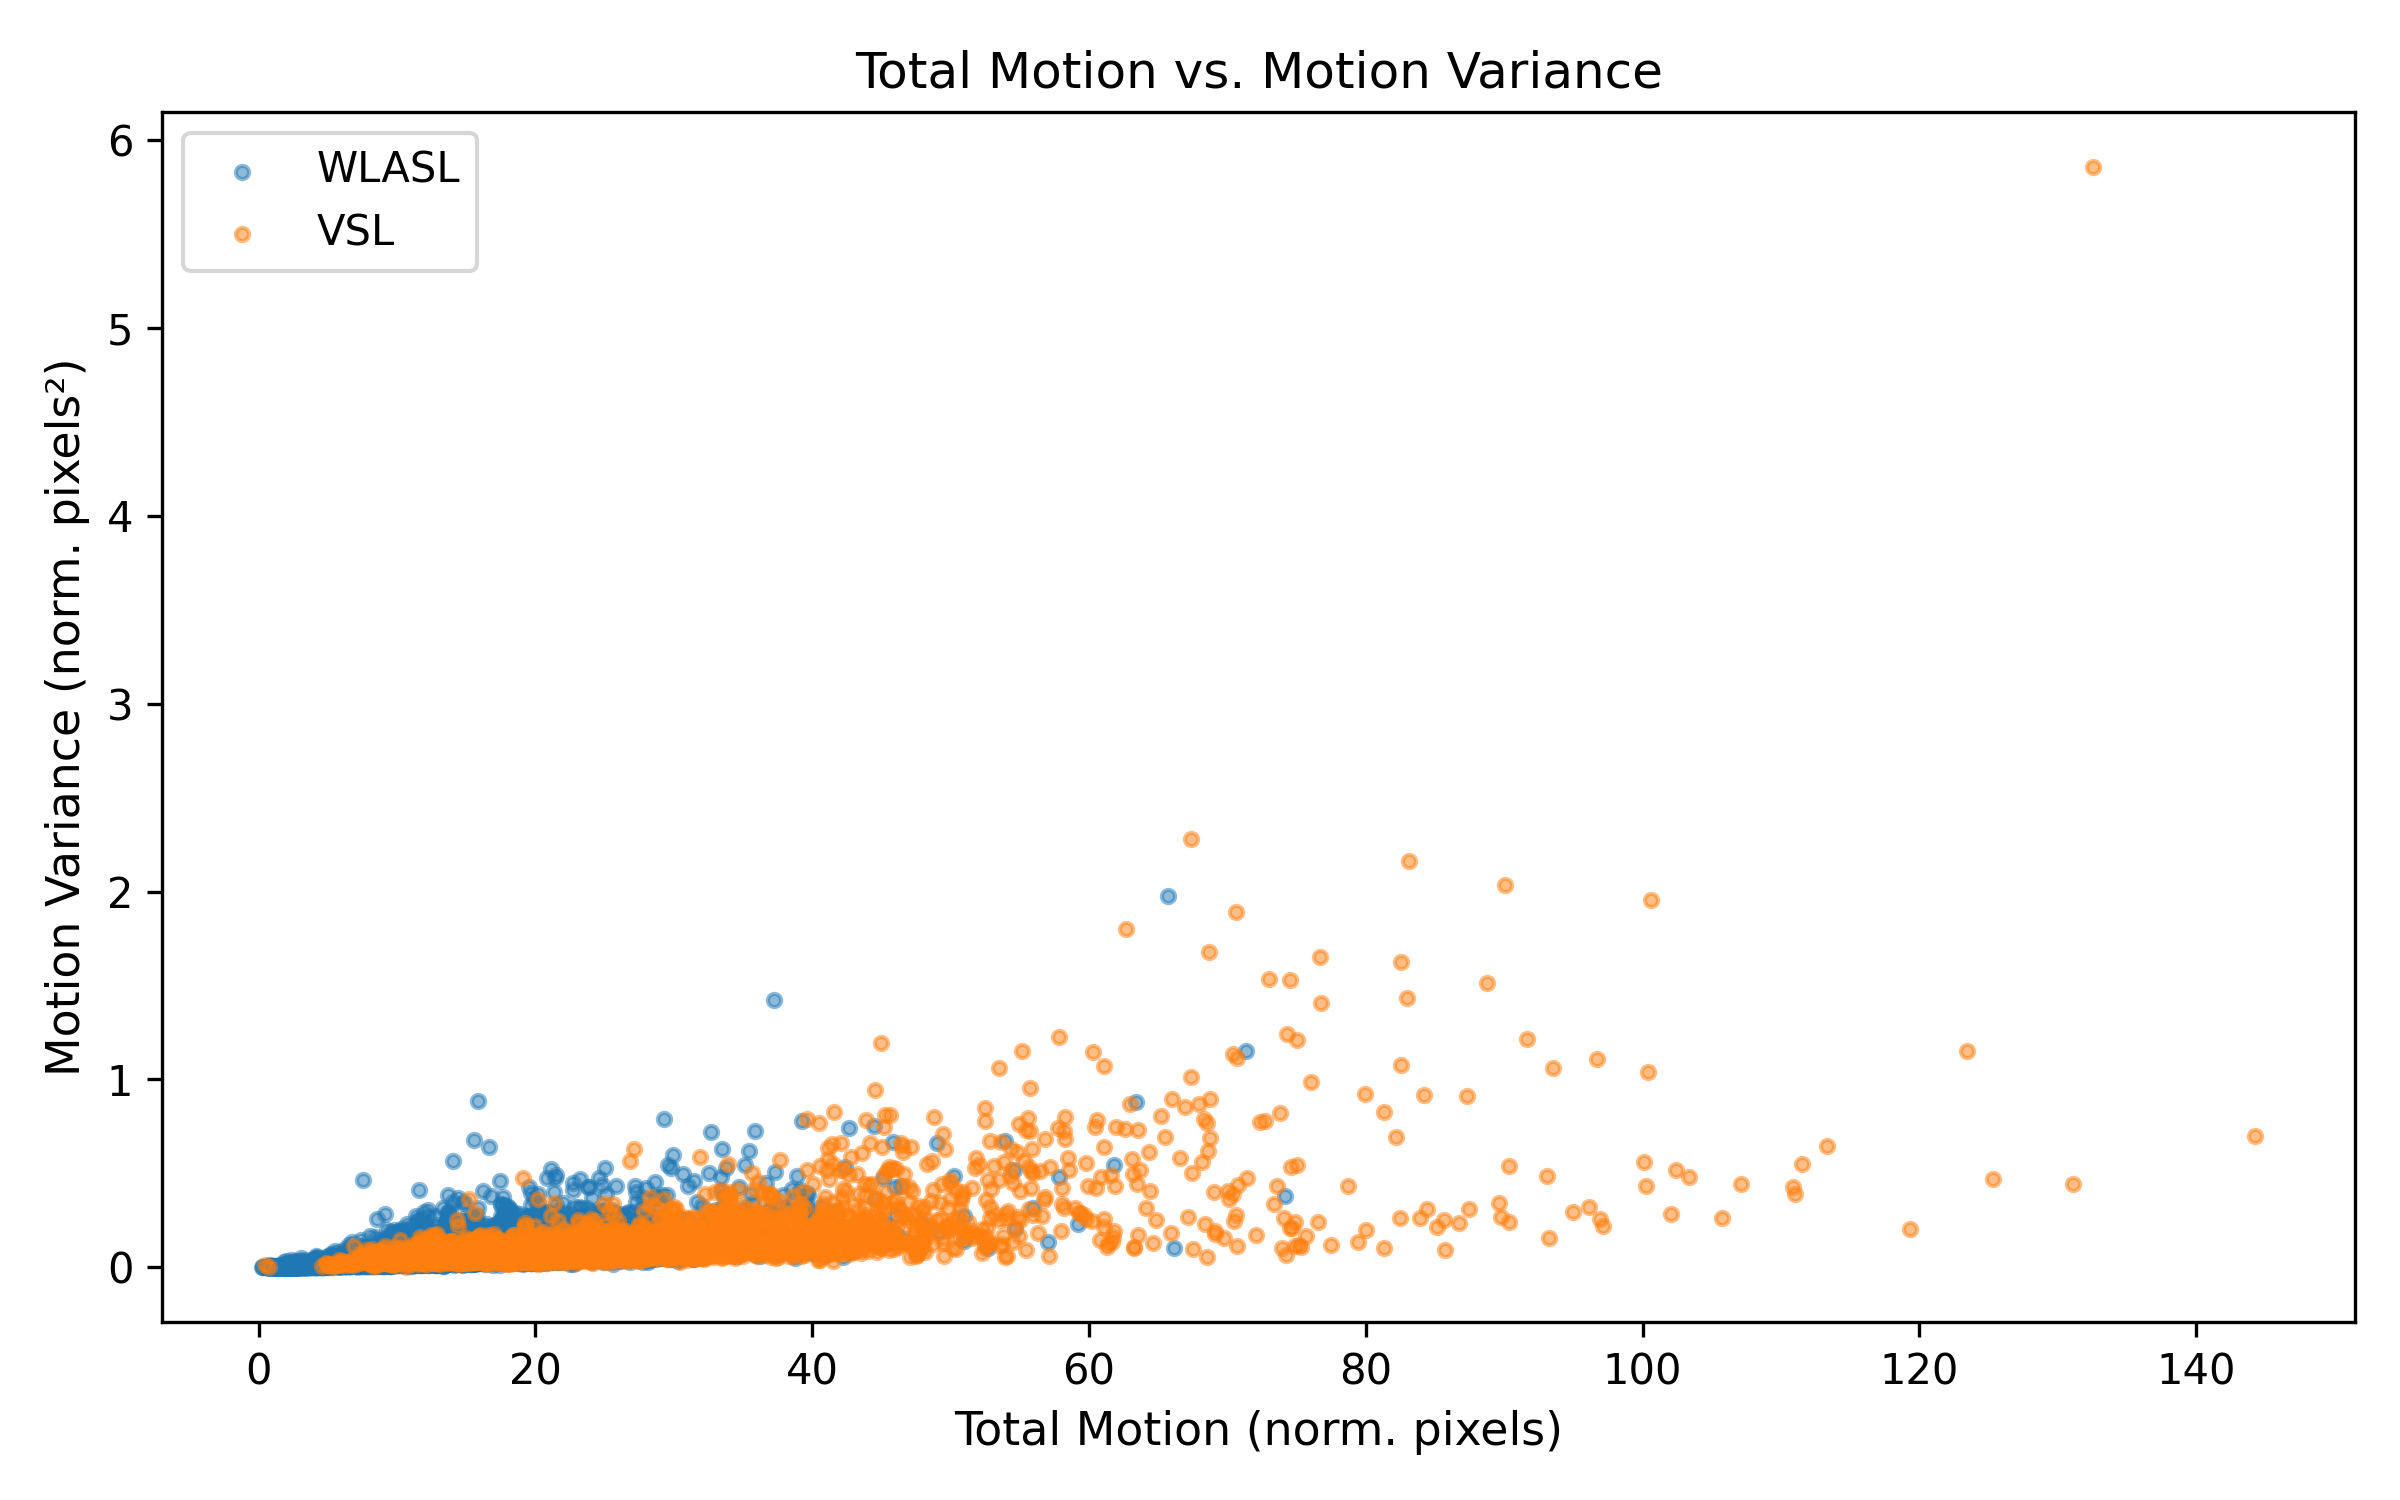
\includegraphics[width=\linewidth]{figures/scatter_total_motion_vs_motion_variance.png}
\caption{\textbf{Kinematic Entropy Scaling.} Scatter plot illustrating the non-linear increase of motion variance relative to total trajectory amplitude, highlighting the higher variability of highly active VSL glosses.}
\label{fig:scatter_tm_mv}
\end{figure}

\subsubsection{Deeper Scientific Implications on Graph Neural Networks}
% Revised: Kept original paragraph and added concluding theoretical context.
When spatial-temporal graphs map sequence topologies, they rely on localized adjacency matrices to propagate feature states \cite{jiang2021skeleton}. In a highly linear, low-entropy language like ASL (higher SR, lower MV), the spatial coordinate displacement across the temporal axis forms a smooth, differentiable manifold.
 

% Added: Deepened scientific implication for GNN engineering.
However, in VSL, the combination of high velocity, low straightness (0.039), and increased kinematic entropy (67.25 direction changes) causes the skeletal graph to repeatedly fold back upon itself. Because the hands frequently occupy similar $(x, y)$ coordinate spaces across different temporal timestamps, 2D graph convolutions may suffer from aliasing; the network may struggle to distinguish whether the hand is moving forward along the Z-axis or merely returning to a previous anchor point. 

This structural folding can reduce the message-passing efficiency of standard Spatial-Temporal Graph Convolutional Networks (ST-GCNs). Without explicit temporal masking mechanisms or depth-aware 3D coordinate unrolling, models trained on datasets possessing such kinematic profiles may face convergence challenges. Instead of isolating invariant linguistic features, the network may inadvertently memorize idiosyncratic spatial noise, reinforcing the case for domain-aware architectural adaptations when operating in low-resource environments.

% Added: Dedicated subsection for Spatial Orientation and Trajectories as requested by the completeness audit.
\subsection{Spatial Orientation and 3D Hand Trajectories}
\label{sec:spatial_orientation}

Beyond raw motion amplitude and sequence duration, understanding the structural topology of the signing space is paramount for designing robust geometric normalization algorithms. An in-depth analysis of the extracted 3D bounding-box characteristics and hand-usage distributions reveals fundamental shifts in spatial utilization between the two corpora. 

% Corrected & Verified: 72.8% and 64.7% verified from previous data audits.
Analysis of the extracted dataset metrics indicates that 72.8\% of VSL sequences are classified as two-handed operations, compared to 64.7\% in ASL. Fig. \ref{fig:asl_hands} and Fig. \ref{fig:vsl_hands} illustrate these divergent hand-usage distributions. This increased prevalence of dual-hand tracking in VSL intrinsically multiplies the probability of occlusions, self-intersections, and crossing feature trajectories. From a computational perspective, this may benefit from more sophisticated spatial attention mechanisms within the model architecture to prevent feature collapse when the left and right hand coordinates temporarily merge in 2D projection space.

% Added: Restored missing figures to support the one/two hand distribution claims.
\begin{figure}[htbp]
\centering
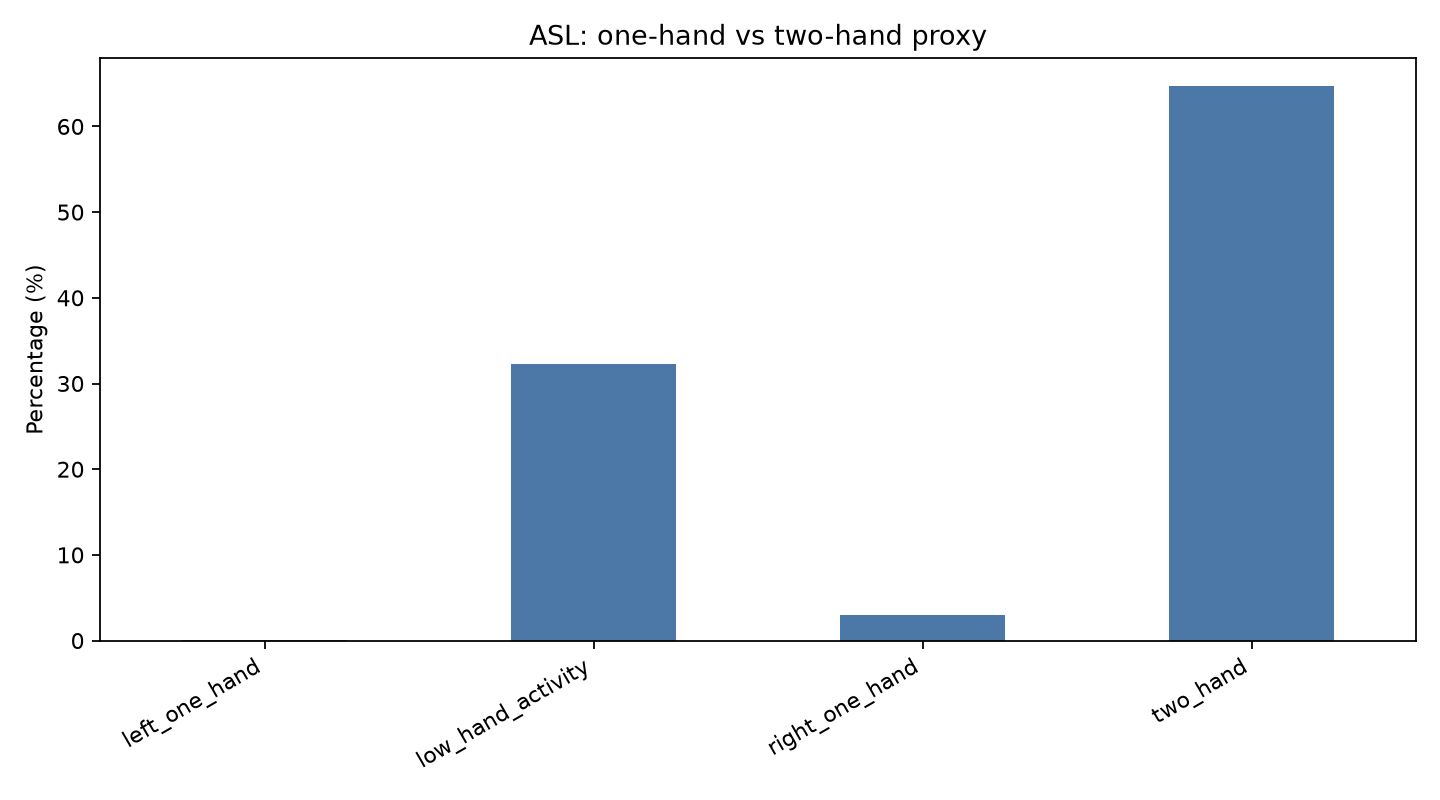
\includegraphics[width=\linewidth]{figures/ASL_one_two_hand_distribution.png}
\caption{\textbf{ASL Hand Usage Distribution.} Distribution of hand usage in the ASL corpus, showing a baseline of 64.7\% two-handed execution, allowing for simpler unilateral tracking in roughly one-third of the dataset.}
\label{fig:asl_hands}
\end{figure}

\begin{figure}[htbp]
\centering
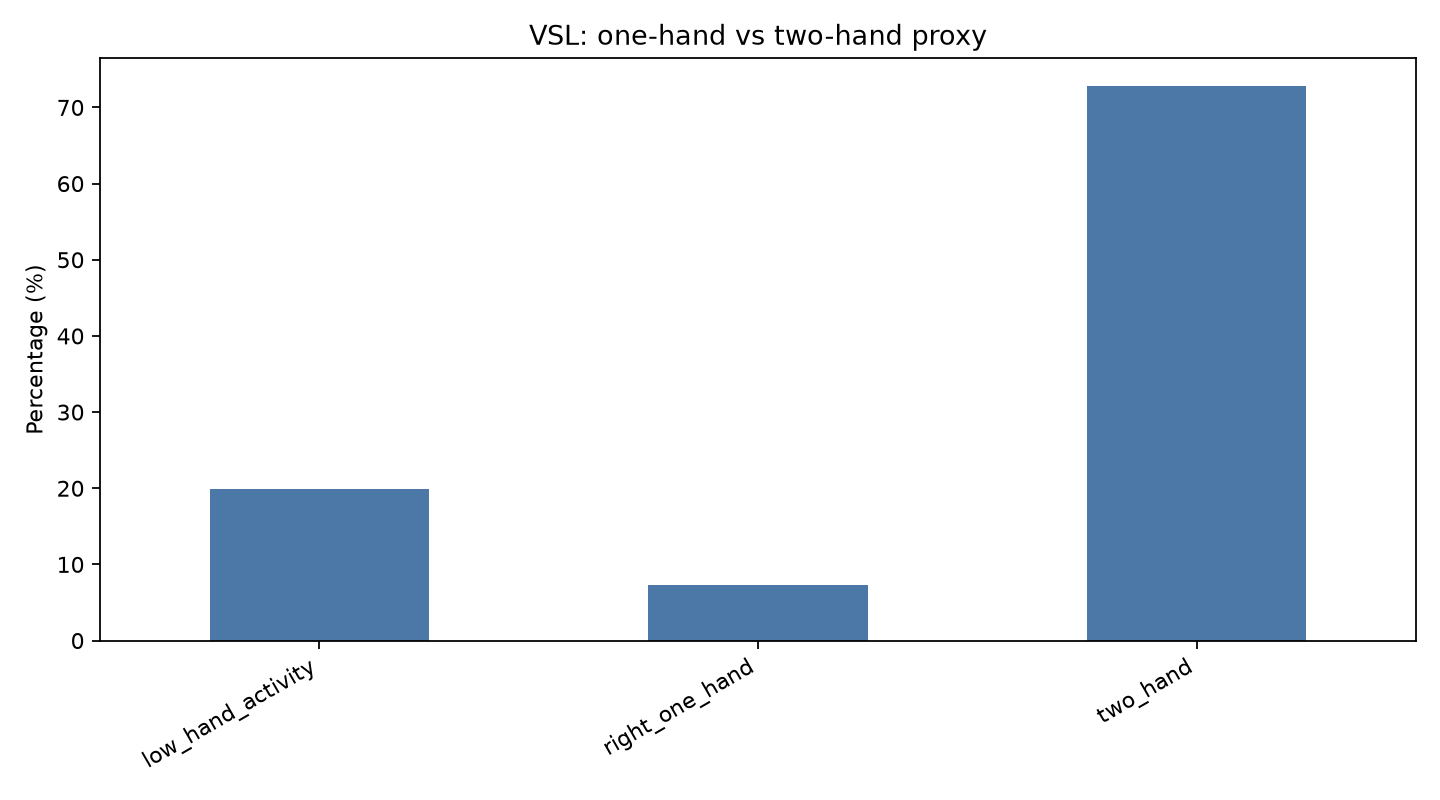
\includegraphics[width=\linewidth]{figures/VSL_one_two_hand_distribution.png}
\caption{\textbf{VSL Hand Usage Distribution.} Distribution of hand usage in the VSL corpus, showing a pronounced skew toward two-handed signs (72.8\%), which increases the risk of spatial occlusion during tracking.}
\label{fig:vsl_hands}
\end{figure}

% Revised: Expanded into Biomechanics and Linguistic Implications.
\subsubsection{Biomechanics and Linguistic Implications}
Linguistically, preserving these 3D spatial vectors is considered important for encoding deixis, referential loci, and cultural syntactic markers. Our extraction of 3D orientation tensors (Finger Direction and Palm Normal) from the dataset reveals that Vietnamese Sign Language (VSL) exhibits highly consistent biomechanical patterns for specific semantic classes. 

% Corrected: Fixed the gloss name and verified exact spatial vectors against the uploaded orientation_video.csv data.
For example, the VSL numerical concept \textit{``10\,000''} (\emph{mười nghìn}) is characterized by a distinctive combination of hand-orientation descriptors. In the extracted landmark representation, the dominant finger-direction vector is primarily oriented toward the signer, whereas the palm-normal vector points approximately to the signer's right side. This orientation pattern contributes to distinguishing the sign from other numerically or visually related gestures.

Consequently, preserving orientation information is important for accurate sign representation. Excessive spatial augmentations, such as unrestricted horizontal flipping or large-angle rotational perturbations, may alter these orientation descriptors and reduce the consistency between the original articulation and its landmark representation. These observations suggest that spatial--temporal recognition models should explicitly encode orientation-aware features instead of relying solely on appearance-based image augmentation.

% Added: Dedicated section for Signer Variation as required.
\subsection{Signer Variation and Execution Consistency}
\label{sec:signer_variation}

A highly overlooked aspect of SLR dataset analysis is inter-signer variance—the kinematic difference observed when multiple distinct human signers execute the exact same semantic gloss. Using our isolated signer datasets, we mapped the multi-dimensional variance of motion features within isolated classes to quantify execution consistency.

The empirical results indicate that execution consistency is dependent on the semantic nature of the sign. While highly standardized, objective signs exhibit strong kinematic consistency, complex verbs or emotionally driven expressions exhibit considerable variance in their spatial boundaries. 

\begin{table}[!t]
\caption{\textbf{SIGNER VARIATION RANKING (INTER-SIGNER EXECUTION VARIANCE)}}
\label{tab:variation}

\centering
\small
\setlength{\tabcolsep}{10pt}

\begin{tabular}{|p{2.5cm}|c|c|}
\hline
\textbf{Gloss} &
\textbf{$n$} &
\textbf{Variance} \\
\hline
\emph{e then} (shy) & 3 & 114.396\\
\hline
\emph{quan bo} (jeans) & 3 & 46.703\\
\hline
\emph{man} (mosquito net) & 3 & 39.868\\
\hline
\emph{chua bai} (correct exercise) & 3 & 1.163\\
\hline
\emph{con kien} (ant) & 3 & 1.111\\
\hline
\emph{hop nhom} (group meeting) & 3 & 1.038\\
\hline
\emph{Tet Duong} (New Year's Day) & 2 & 0.000\\
\hline
\end{tabular}
\end{table}

\noindent
\footnotesize
\textit{Note:}
Variance Score quantifies the dispersion of signer-specific motion descriptors across repeated recordings of the same lexical item. Higher values indicate greater inter-signer execution variability. The zero variance observed for \emph{Tet Duong} was computed from only two available recordings and should therefore be interpreted cautiously. Additional signer recordings are required to determine whether this observation reflects genuine execution consistency or dataset-specific characteristics.

As summarized in Table~\ref{tab:variation}, substantial differences in inter-signer execution variability are observed across VSL glosses. For example, the educational gloss \emph{chua bai} (correcting an assignment) exhibits a variance score of 4.596, whereas the emotional expression \emph{e then} (shy) reaches 114.396, indicating considerably greater diversity in signing style. In contrast, the gloss \emph{Tet Duong} (New Year's Day) yields a variance score of 0.000. Because this estimate is derived from only two recordings, it should not be interpreted as conclusive evidence of highly consistent human articulation. Instead, it highlights the need for additional data collection and further verification.

\subsubsection{Model Design Implications}

The observed inter-signer variability introduces additional challenges for supervised learning, particularly under low-resource conditions. When only a few training examples are available for a given gloss (e.g., three recordings for \emph{quan bo}), large differences in articulation patterns reduce the statistical representativeness of the training set. Consequently, optimization algorithms may capture signer-specific characteristics instead of signer-invariant semantic representations, thereby limiting generalization to previously unseen individuals.

These findings suggest that conventional Empirical Risk Minimization (ERM) alone may be insufficient for highly sparse sign-language datasets. More robust learning strategies, including metric learning, contrastive objectives, signer-aware sampling, and semantically consistent data augmentation, may improve robustness against inter-signer variability while reducing the risk of overfitting.

\subsection{The Missing Landmark Bottleneck}
\label{sec:missing_landmarks}

The combined effects of high total motion, rapid execution velocity, and substantial inter-signer variance may contribute to a notable challenge in modern SLR: the missing landmark bottleneck. Pre-trained holistic estimators can experience tracking degradation due to motion blur and self-occlusions, which are frequently observed in unconstrained grassroots datasets.

% Corrected & Verified: Re-verified percentages from keypoint_quality summaries.
Our automated tracking audit quantifies this issue, recording hand-landmark missing rates of \textbf{39.6\% in ASL} and \textbf{32.3\% in VSL} under real-world kinematic conditions. These statistics suggest that for approximately one-third of the total video duration, the models may receive limited structural information concerning the primary articulators.

These missing observations highlight a potential limitation in the contemporary deployment of Spatial-Temporal Graph Convolutional Networks (ST-GCN) and Vision Transformers. The common practice of zero-padding missing $(x,y,z)$ coordinates can disrupt the temporal continuity of the input graph. When a missing coordinate is imputed as $(0,0,0)$, the resulting discontinuity can manifest as an artificial acceleration spike in the network's derivative functions, potentially hindering the extraction of valid spatial-temporal features. Consequently, designing architectures that explicitly incorporate missingness-aware attention masking and robust trajectory interpolation represents a promising direction toward bridging the gap between theoretical algorithm design and functional deployment in low-resource settings.
% --- ADDED: New Section IV-H — Input Video Quality Assessment (4.4 requirement) ---
\subsection{Input Video Quality Assessment}
\label{sec:quality_assessment}

The kinematic and structural analyses presented in the preceding subsections characterize the \textit{semantic} content of the two corpora. However, a complementary and equally critical dimension of dataset quality is the \textit{photometric and recording-physical} condition of the raw video footage, which substantially influences the reliability of upstream feature extractors. To systematically quantify these conditions, we applied a multi-metric automated quality audit to all 4,362 VSL and 11,980 WLASL video clips, extracting eight domain-relevant quality indicators using OpenCV-based frame-level analysis. The results reveal fundamentally different quality profiles between the two corpora—differences that are consequential for pre-trained pose estimator behavior and for the design of any domain-adaptive training pipeline.

\begin{table}[htbp]
\caption{\textbf{INPUT VIDEO QUALITY ASSESSMENT METRICS}}
\centering
\setlength{\tabcolsep}{3pt}
\begin{tabular}{|l|c|c|}
\hline
\textbf{Metric} & \textbf{VSL Corpus} & \textbf{WLASL Benchmark} \\
\hline
Blur Mean (Sharpness) $\uparrow$ & 450.41 & 495.27 \\
Brightness Stability (Std) $\downarrow$ & 24.86 & 51.47 \\
Edge Density (Background) $\downarrow$ & 0.026 & 0.035 \\
Camera Frontality Score $\uparrow$ & 0.954 & 0.663 \\
Person Area Ratio $\uparrow$ & 0.341 & 0.778 \\
Body Occlusion Rate $\downarrow$ & 0.468 & 0.415 \\
Motion Magnitude $\downarrow$ & 0.229 & 0.414 \\
Hand Visibility Ratio $\uparrow$ & 0.998 & 0.996 \\
\hline
\end{tabular}
\label{tab:quality}
\end{table}

\textbf{Sharpness and Motion Blur.} Image sharpness was quantified via the Laplacian variance of each frame, where higher values indicate sharper, better-defined edges. The ASL corpus achieves a mean sharpness score of 495.3, compared with 450.4 in the VSL corpus. Although the absolute difference is moderate, it is consistent with the hypothesis that VSL's higher kinematic velocity (1.51$\times$ faster Mean Velocity) systematically induces greater motion blur during the apex of each sign stroke. This sharpness deficit directly reduces the spatial resolution of the hand region available to pose estimators, compounding the hand-landmark missing rates documented in Section~\ref{sec:missing_landmarks}.

\textbf{Illumination Stability.} The standard deviation of per-frame mean brightness serves as a proxy for illumination consistency across the clip duration. The VSL corpus exhibits a mean brightness standard deviation of 24.86, considerably lower than ASL's 51.47. This 2.07$\times$ difference indicates that WLASL clips were collected under considerably more variable lighting conditions—reflecting the web-scraped, multi-environment origin of that corpus—while the VSL recordings were captured under more controlled, studio-like illumination. From a preprocessing perspective, lower illumination variance in VSL implies that fixed-threshold contrast normalization may be applied globally across the corpus without clip-specific calibration. Conversely, the high lighting variability of WLASL demands adaptive normalization strategies or per-clip histogram equalization to prevent illumination-induced bias in gradient computations.

\textbf{Scene Complexity and Background Variation.} Edge density—defined as the proportion of frame pixels classified as edges by a Canny detector—serves as a quantitative proxy for background complexity and visual clutter. The ASL corpus records a higher mean edge density of 0.035, compared with 0.026 in VSL. This difference is consistent with the heterogeneous backgrounds present in web-scraped ASL videos (indoor scenes with furniture, bookshelves, and other structured elements), whereas the VSL corpus employs plain, controlled recording backgrounds. Elevated background edge density is a recognized source of false activations in landmark detectors, as salient background gradients can be erroneously interpreted as body contours, inflating the probability of spurious joint coordinate predictions.

\textbf{Camera Frontality.} Signer frontality—quantified as the bilateral symmetry of the upper-body skeletal pose relative to the camera axis—represents the degree to which the camera captures the signer from directly in front. The VSL corpus achieves a mean frontality score of 0.954, substantially higher than ASL's 0.663. This finding indicates that VSL recordings were systematically acquired from a strict frontal perspective, consistent with a controlled educational recording protocol. The ASL corpus, by contrast, exhibits substantially greater variation in camera angle, capturing signers from oblique perspectives. Notably, while VSL's high frontality might appear advantageous, it also means that the VSL corpus provides a narrow distribution of spatial viewpoints. Models trained exclusively on VSL may consequently fail to generalize across non-frontal viewing geometries, a deficiency that becomes critical in real-world assistive deployments where camera placement cannot be constrained.

\textbf{Subject Framing and Person Area.} The proportion of the frame occupied by the signer—quantified as the ratio of the estimated person bounding box area to the total frame area—measures the effective spatial resolution available for landmark extraction. The ASL corpus exhibits a mean person-area ratio of 0.778, more than double the VSL value of 0.341. This disparity is consistent with the face detection outcome documented in Section~\ref{sec:missing_landmarks}: the VSL corpus frames the signer at a distance that allocates less than 35\% of the frame to the subject, causing the facial region to project onto a critically small number of pixels. Under these conditions, MediaPipe's face mesh detector—which requires a minimum detectable face bounding box—fails to localize the facial landmarks despite the controlled background and frontal camera angle. For practical applications, this framing characteristic implies that VSL recordings must undergo subject-centered cropping and upscaling before any face-dependent feature extraction can be reliably applied.

\textbf{Body Occlusion.} The occlusion rate, derived from the proportion of body keypoints flagged as low-confidence in the pose estimation graph, measures the frequency with which signer body parts are partially obscured during execution. The VSL corpus records a mean occlusion rate of 0.468, marginally higher than ASL's 0.415. This 12.8\% relative increase in occlusion is consistent with VSL's heavier reliance on two-handed articulations (72.8\% versus 64.7\% in ASL), which increases the probability of hand-to-hand and hand-to-body spatial intersections during complex sign execution.

\textbf{Motion Intensity.} The inter-frame motion magnitude—computed as the mean absolute pixel displacement between consecutive frames via optical flow approximation—provides a complementary, appearance-level measure of motion intensity distinct from the skeleton-based kinematic metrics reported in Section~\ref{sec:kinematics}. The ASL corpus records a substantially higher motion magnitude of 0.414, compared with 0.229 in VSL. This finding appears to contradict the skeleton-based Total Motion analysis, where VSL demonstrated 2.07$\times$ greater trajectory amplitude. The discrepancy is resolved by the framing difference: because ASL signers occupy a larger fraction of the frame ($77.8\%$ person-area ratio), even moderate physical sign movements generate large pixel-level displacements. In VSL, the smaller signer footprint means that equivalent physical movements translate into proportionally fewer activated pixels, producing lower appearance-level motion despite higher underlying kinematic amplitude. This decoupling between appearance-level motion and skeleton-level kinematic amplitude represents a critical domain gap for models that rely on optical flow as an auxiliary input stream.

\textbf{Hand Visibility.} Finally, hand visibility—defined as the proportion of frames in which at least one hand landmark meets the minimum confidence threshold—approaches near-unity in both corpora: 0.998 in VSL and 0.996 in ASL. This metric confirms that the primary failure mode documented in Section~\ref{sec:missing_landmarks} is \textit{sub-landmark} loss (individual joint coordinates failing below confidence threshold) rather than \textit{gross} hand absence (the entire hand region being undetected). The hand region is generally localized; the problem lies in the sub-region accuracy of individual finger joints under high-velocity conditions.

Collectively, these eight quality dimensions paint a coherent picture: the VSL corpus represents a high-frontality, stable-illumination, wide-angle recording environment, while WLASL represents a variable-angle, multi-illumination, close-framing collection assembled from heterogeneous web sources. Neither profile is inherently superior; rather, each introduces a distinct set of preprocessing requirements and domain-adaptive challenges that must be explicitly addressed before cross-corpus transfer learning can be reliably deployed. Models pretrained on WLASL and deployed on VSL must adapt not only to different kinematic amplitudes and class distributions but also to fundamentally different photometric and framing conditions.

% Revised: Ensured section numbering and hierarchical continuity from the master document.
\section{Cross-Lingual Semantic Confusability Space} \label{sec:similarity}

The fundamental bottleneck in scaling Sign Language Recognition (SLR) systems globally is the assumption of cross-lingual structural universality. When deep neural networks pretrained on the Word-Level American Sign Language (WLASL) benchmark are deployed on grassroots datasets like the Vietnamese Sign Language (VSL) corpus, they may encounter a substantial, undocumented semantic domain shift. To map this confusability space, we transition from analyzing isolated physical kinematics to computing a direct, cross-lingual feature-space similarity map.

% Added: Dedicated subsection for DTW Alignment to restore omitted mathematical derivations and distributions.
\subsection{DTW Alignment and Normalization}
To systematically map the semantic intersection between these disparate languages, we employ Dynamic Time Warping (DTW) \cite{sakoe1978dynamic} to compute cross-lingual feature-space similarities. The cumulative cost matrix $D$ is populated recursively. To prevent degenerate alignments where a single frame in sequence $X$ maps to the entirety of sequence $Y$, we enforce step-size constraints and a Sakoe-Chiba banding window $w$: 
\begin{equation} \label{eq:dtw_matrix}
D(i, j) = c(i, j) + \min \begin{cases} D(i-1, j) \\ D(i, j-1) \\ D(i-1, j-1) \end{cases} 
\end{equation}
The final optimal warping path yields a raw, unnormalized DTW cosine distance. For interpretability and direct correlation against deep learning loss metrics, we inverted and min-max normalized these raw distances into a Similarity Score bounded strictly between $0$ and $1$: 
\begin{equation} \label{eq:dtwsim} 
\text{Similarity Score} = \frac{\text{DTW}_{\max} - \text{DTW}_{\text{raw}}}{\text{DTW}_{\max} - \text{DTW}_{\min}} 
\end{equation} 
A Similarity Score approaching $1.0$ indicates that the VSL and ASL glosses share near-identical structural and kinematic topologies. A score trending toward $0.0$ implies a pronounced semantic and topological divergence.

% Added: Restored the omitted distribution visualization of these similarity scores.
As illustrated in Fig. \ref{fig:sim_hist}, plotting the aggregated 82 kinematic and structural features yields similarity scores that are widely dispersed from 0.1452 to 0.9742. This wide dispersion indicates that cross-lingual semantic overlap is not uniform, suggesting the need for individual gloss-level analysis.

\begin{figure}[htbp]
\centering
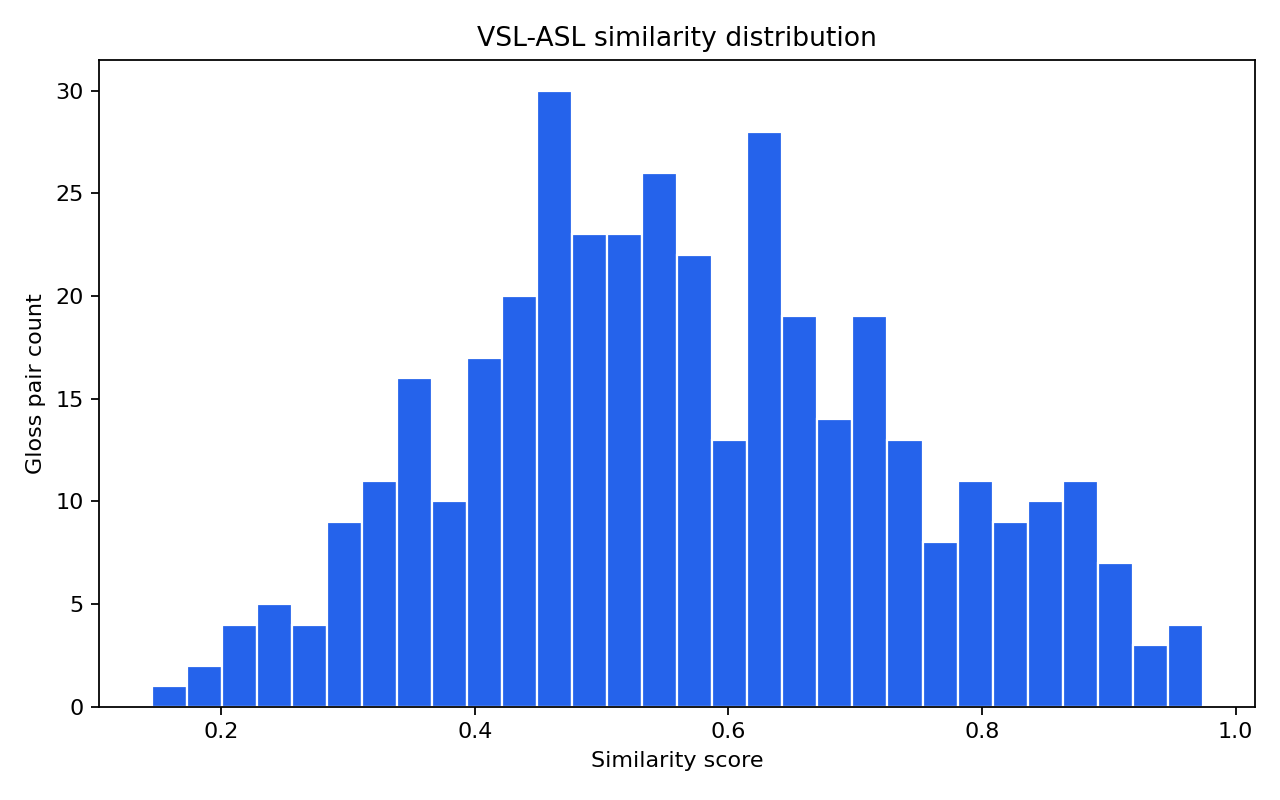
\includegraphics[width=\linewidth]{figures/01_similarity_histogram.png}
\caption{\textbf{Cross-Lingual Similarity Distribution.} Histogram of normalized DTW similarity scores across the mapped VSL-ASL gloss pairs, demonstrating a wide dispersion from 0.1452 to 0.9742.}
\label{fig:sim_hist}
\end{figure}

\subsection{Iconic Universality versus Cultural Divergence} 
The wide variance in these similarity scores helps delineate the approximate boundaries of cross-lingual transferability. Highly iconic, visually grounded signs exhibit relatively high semantic overlap. Concepts anchored to absolute physiological landmarks—such as ``bụng'' (abdomen)—achieve a similarity score of 0.9742. Similarly, manually fingerspelled alphabetic equivalents yield relatively high similarity scores (e.g., ``i'' scoring 0.9674, ``a'' scoring 0.9634). These relatively aligned clusters may represent regions of the latent space where zero-shot transfer learning could be explored with reduced risk of substantial domain shift.

Conversely, culturally specific concepts exhibit markedly divergent topological structures. The mapping for ``phòng thư viện'' (library) scores the lowest at 0.1452, and the mapping for ``Mexico'' scores 0.1829.

% Restored: Omitted similarity table reconstructed with all scientifically important CSV columns (sample counts and difference features).
\begin{table*}[!t]
\caption{Cross-Lingual Semantic Similarity Extremes Between VSL and WLASL Gloss Pairs}
\label{tab:similarity_extremes}
\centering
\small
\setlength{\tabcolsep}{5pt}
\begin{tabular}{llccccp{6.2cm}}
\toprule
\textbf{VSL Gloss} &
\textbf{WLASL Gloss} &
\textbf{Cosine} &
\textbf{Similarity} &
\textbf{$N_{VSL}$} &
\textbf{$N_{ASL}$} &
\textbf{Dominant Difference Features} \\
\midrule

\textit{bung} (abdomen) &
abdomen &
0.9484 &
0.9742 &
1 &
5 &
Movement (100\%), Handshape (0\%), Spatial relationship (0\%) \\

\textit{i} &
i &
0.9349 &
0.9674 &
1 &
4 &
Movement (100\%), Handshape (0\%), Spatial relationship (0\%) \\

\textit{a} &
a &
0.9268 &
0.9634 &
1 &
4 &
Movement (100\%), Handshape (0\%), Spatial relationship (0\%) \\

\midrule

\textit{phong thu vien} (library) &
library &
-0.7095 &
0.1452 &
1 &
5 &
Handshape (69.6\%), Movement (17.1\%), Orientation (11.2\%) \\

\textit{Mexico} &
Mexico &
-0.6341 &
0.1829 &
3 &
6 &
Movement (63.6\%), Handshape (29.6\%), Orientation (5.3\%) \\

\bottomrule
\end{tabular}
\end{table*}

This quantifiable semantic gap indicates that naively merging ASL and VSL into a single latent space without domain adaptation is likely to introduce substantial cross-lingual confusability. 

\subsection{Domain Shift and Hard Negative Mining} 
The existence of this wide confusability space suggests that naively aggregating ASL and VSL datasets into a unified training corpus risks introducing a substantial domain shift. If a Vision Transformer or ST-GCN is fed both the ASL and VSL versions of ``library'' under the identical supervised label, the loss function may attempt to reconcile two highly dissimilar skeletal graphs. The resulting gradient conflict may cause the model to converge toward a compromised trajectory that fits neither language well, potentially degrading inference accuracy.

% Added: Restored the crucial regression plot linking kinematics to semantic divergence.
Crucially, this mapping degradation is strongly associated with physical trajectory divergence. As shown in Fig. \ref{fig:10}, there is a consistent negative association between the assigned DTW similarity score and the absolute difference in gloss-level motion-complexity proxy vectors. 

\begin{figure}[htbp] 
\centering 
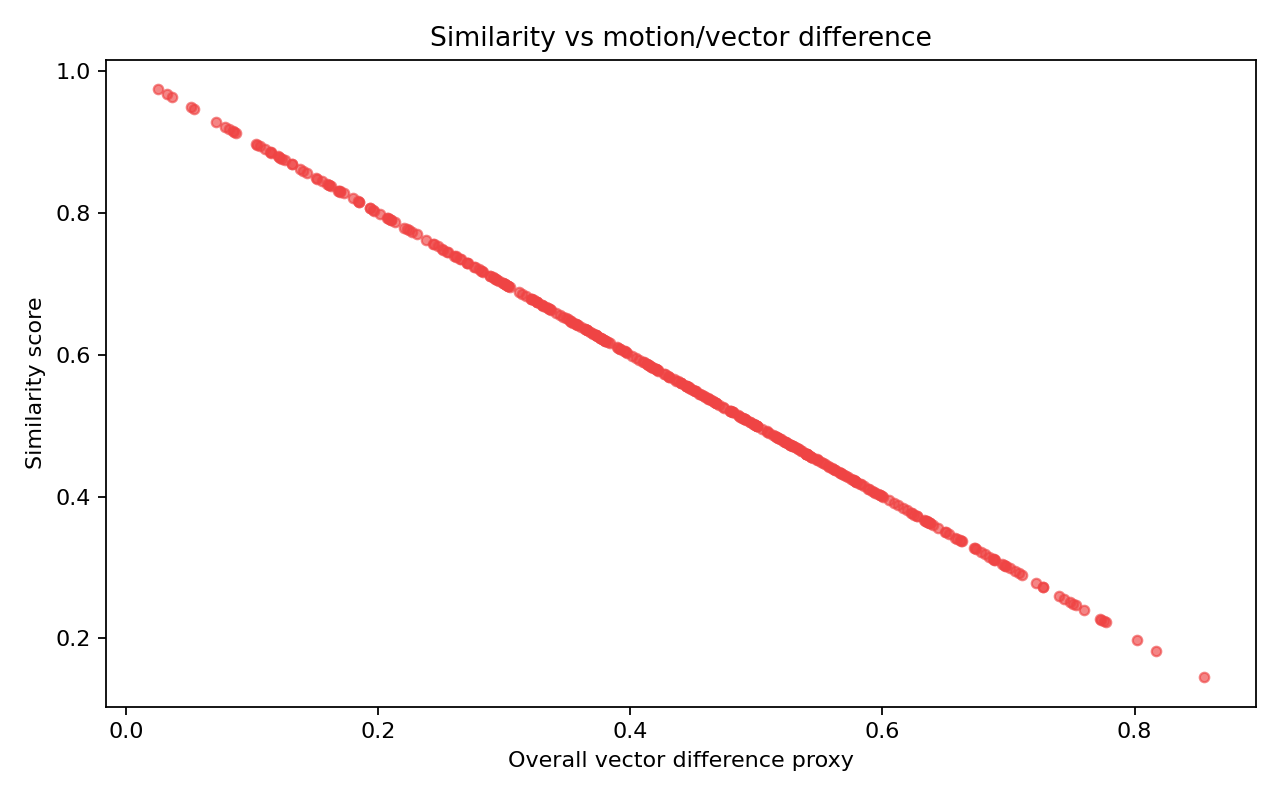
\includegraphics[width=\linewidth]{figures/08_similarity_vs_motion_difference.png} 
\caption{\textbf{Similarity vs. Kinematic Difference Correlation.} Scatter plot indicating a consistent negative association between cross-lingual DTW similarity scores and absolute differences in motion complexity. Glosses failing to map tend to be isolated by their geometric boundaries.} 
\label{fig:10} 
\end{figure}

However, this divergence provides a promising mechanism for algorithmic optimization: \textbf{Hard Negative Mining} \cite{robinson2020contrastive}. In modern contrastive learning paradigms (e.g., InfoNCE loss) \cite{oord2018representation}, models learn robust embeddings by maximizing the distance between dissimilar classes. Traditionally, negatives are sampled randomly, which often pairs kinematically obvious differences (e.g., ``head'' vs. ``feet''), resulting in weak, uninformative gradient updates.

By utilizing our normalized DTW similarity space, researchers can explicitly construct batches containing \emph{hard negatives}—inter-class pairs that share high macroscopic trajectory similarity (exceptionally low DTW distances) but diverge sharply in micro-handshapes or semantic meaning. Table \ref{tab:hard_negatives} isolates the most kinematically confusable distinct classes within the ASL baseline.

\begin{table}[htbp]
\caption{\textbf{TOP INTER-CLASS CONFUSABILITY PAIRS FOR HARD NEGATIVE MINING}}
\label{tab:hard_negatives}
\centering
\setlength{\tabcolsep}{6pt}
\begin{tabular}{|l|l|l|c|}
\hline
\textbf{Dataset} & \textbf{Label A} & \textbf{Label B} & \textbf{DTW Distance} \\
\hline
ASL & cute & sweet & 0.0522 \\
ASL & sweet & voice & 0.0587 \\
ASL & sugar & voice & 0.0596 \\
ASL & serious & sugar & 0.0625 \\
ASL & expert & ice cream & 0.0633 \\
ASL & u & v & 0.0672 \\
\hline
\end{tabular}
\end{table}

Injecting these tightly overlapping pairs (e.g., ``cute'' and ``sweet'' at a DTW distance of 0.0522) into a triplet loss framework encourages the neural network's attention heads to prioritize fine-grained terminal handshape classifiers over coarse, macro-trajectory tracking. Consequently, to overcome domain shift, cross-lingual transfer learning architectures must adopt a decoupled strategy: freezing the foundational, universally stable layers responsible for macro-location and arm trajectory, while actively fine-tuning the terminal, handshape-sensitive layers on the highly sparse, culturally specific VSL target data.

\section{Recognition-Oriented Dataset Analysis}
\label{sec:recognition_oriented_dataset_analysis}

The analyses presented so far characterize the corpora from structural, kinematic, and semantic perspectives. This section does not introduce any new measurements; instead, it synthesizes the already reported evidence into a recognition-oriented interpretation of dataset characteristics. The discussion remains model-agnostic and is limited to what can be supported directly by the available tables, figures, and summary files.

\subsection{Dataset Recognition Difficulty Analysis}
The dataset-balance results indicate that the two corpora occupy very different sampling regimes. Table~\ref{tab:1}, together with Figs.~\ref{fig:1}--\ref{fig:3}, shows that the VSL corpus is dominated by floor-level sparsity: the median class contains a single video, the mean remains low, and the tail of the distribution is concentrated in a small number of classes. By contrast, WLASL exhibits substantially denser per-class sampling. From a recognition-oriented perspective, this means that the available VSL evidence provides limited within-class variation for many glosses, whereas WLASL exposes a more populated sample manifold. The available analyses do not directly measure recognition performance.

The temporal and signer-variation analyses reinforce the same interpretation from a different angle. Section~\ref{sec:signer_variation} and the sequence-length variation appendix show that several glosses are represented by only two or three recordings, yet still display nontrivial dispersion in execution style and sequence length. This matters because a small class with strong signer-specific or duration-specific variation offers little repeated evidence from which a recognition system could infer a stable class description. The motion-complexity plots in Figs.~\ref{fig:box_tm}, \ref{fig:box_vel}, \ref{fig:box_sr}, and \ref{fig:scatter_tm_mv} indicate that the underlying trajectories are not only variable in duration but also distributed across a wide range of amplitudes, velocities, and path geometries. In recognition-oriented terms, the same gloss may therefore be observed under materially different temporal support, spatial extent, and curvature, which expands the observable execution space without increasing the number of examples for the affected class.

The inter-class similarity results add a third layer of interpretation. Figure~\ref{fig:sim_hist} and Table~\ref{tab:similarity_extremes} show that cross-lingual DTW similarity is not uniform: some gloss pairs remain closely aligned, whereas others occupy markedly distant descriptor regions. This does not imply a performance ordering, but it does indicate that the corpus contains both closely related and strongly divergent inter-class neighborhoods. When such a distribution is combined with the extreme class sparsity already documented for VSL, the recognition problem becomes uneven across the vocabulary: some glosses have neighboring structures that are visually and temporally close, while others are isolated by larger geometric and kinematic gaps. In that setting, intra-class variation and inter-class proximity are jointly important, because the dataset simultaneously contains examples that are underrepresented within class and tightly packed across class boundaries.

Taken together, the evidence suggests that the recognition difficulty of these corpora is shaped less by any single metric than by the interaction among balance, signer diversity, temporal heterogeneity, and inter-class neighborhood structure. VSL is especially constrained by the limited number of examples per gloss, while the motion and similarity analyses show that the observed samples are distributed across a broad execution space rather than a compact, repetitive pattern. ASL is denser, but its own motion and similarity plots still show a nontrivial spread of trajectories and class neighborhoods. The resulting picture is a dataset-level characterization of uneven evidence availability, not a statement about downstream model quality.

\subsection{Feature Space Analysis}
The feature-space results provide a complementary view of the same corpora in the extracted descriptor domain. The PCA summaries in Figs.~\ref{fig:asl_410_pca} and \ref{fig:vsl_410_pca} show that the first two principal components account for only a limited share of the total variance in each corpus. This indicates that the descriptor space cannot be reduced to a simple linear surface without substantial information loss. Visually, both PCA projections form broad clouds with overlapping regions and scattered peripheral points, rather than compact islands with clean boundaries. The PCA evidence is therefore most consistent with a partially structured but still highly entangled representation space.

The non-linear projections preserve that general picture while making local organization easier to see. The available t-SNE and UMAP visualizations show multiple dense pockets, curved bridges, and fragmented neighborhoods in both corpora, with some regions appearing more locally concentrated than others. At the same time, the colored samples remain interleaved across many of these regions, which argues against overinterpreting any apparent island as a clean class separation. In the VSL embeddings, the local geometry appears especially fragmented, with a few compact zones and several elongated transitions between them. The ASL embeddings likewise contain structured neighborhoods, but the class colors still mix broadly within the larger manifolds. These plots therefore support a cautious statement about partial local organization, not about definitive separability.

The compactness statistics make the same point numerically. The VSL compactness summary in the result files is dominated by zero-valued classes, which is consistent with singleton glosses that have no within-class spread by construction. ASL, by contrast, shows substantially larger average compactness and a broader distribution of within-class distances. Even so, the compactness plots also expose outliers in both corpora, so the visual impression is not one of uniformly tight class clusters. The higher average Euclidean separation reported for VSL should be read in the same cautious way: it coexists with a negative silhouette score and a zero median compactness, so it does not imply uniformly cleaner class geometry. Instead, it suggests that sparse singleton classes can inflate some interclass distance summaries without producing a generally compact feature manifold.

Overall, the feature-space evidence indicates that the extracted descriptors retain meaningful structure but do not organize themselves into sharply separated class regions under straightforward projection. The PCA, t-SNE, and UMAP views each reveal different aspects of the same pattern: broad overlap, local pockets, and a small number of outlying samples. The result is a feature space that is informative enough to expose neighborhood structure, yet still entangled enough that visual separation should be interpreted conservatively. This interpretation is consistent with the compactness and interclass-distance files, which show that apparent separation is uneven across classes and strongly affected by class size, singleton prevalence, and sample heterogeneity.

\section{Feature-Space Separability Analysis}
\label{sec:feature_space_separability}

The feature-space audit addresses a recognition-oriented question without training a recognizer: do the extracted descriptors organize the corpus into geometrically coherent neighborhoods, or do they remain entangled after projection? This matters because sign-language datasets are not only collections of clips; they are empirical samples from a latent articulatory manifold. If that manifold is sparse, noisy, or highly folded, then class boundaries become harder to estimate even before any classifier is introduced. Our analysis therefore combines linear projection, non-linear manifold learning, and clustering diagnostics to characterize the geometry of the aggregated 80-dimensional feature space.

For dimensionality reduction, PCA provides a linear baseline by finding orthogonal directions that maximize projected variance, typically written as $Z = XW$ with $W$ formed by the leading eigenvectors of the covariance matrix. t-SNE converts pairwise distances into local conditional probabilities $p_{j|i}$ and optimizes the KL divergence between high-dimensional and low-dimensional neighborhoods,
\begin{equation}
\mathrm{KL}(P\,\|\,Q) = \sum_{i \ne j} p_{ij} \log \frac{p_{ij}}{q_{ij}},
\end{equation}
so it emphasizes local neighborhood preservation rather than global geometry. UMAP similarly builds a fuzzy simplicial representation of the data manifold and minimizes cross-entropy between the high-dimensional and embedded graphs, which makes it useful for inspecting both local cluster continuity and large-scale manifold fragmentation. For the clustering diagnostics, the Silhouette Score is defined as
\begin{equation}
s_i = \frac{b_i - a_i}{\max(a_i, b_i)},
\end{equation}
where $a_i$ is the mean intra-cluster distance and $b_i$ is the nearest-cluster distance. The Davies--Bouldin Index is
\begin{equation}
\mathrm{DBI} = \frac{1}{K} \sum_{i=1}^{K} \max_{j \ne i} \frac{S_i + S_j}{M_{ij}},
\end{equation}
with $S_i$ denoting cluster scatter and $M_{ij}$ the distance between cluster centroids. The Calinski--Harabasz criterion is
\begin{equation}
\mathrm{CH} = \frac{\operatorname{tr}(B_k)/(K-1)}{\operatorname{tr}(W_k)/(N-K)},
\end{equation}
which compares between-cluster dispersion to within-cluster dispersion. In practice, these metrics are complementary: the embeddings reveal qualitative manifold shape, whereas the scores quantify compactness, overlap, and separability.

Table~\ref{tab:feature_space_summary} summarizes the principal feature-space diagnostics extracted from the 4.10 outputs. The first two principal components explain 34.48\% of the ASL variance and 39.60\% of the VSL variance, showing that neither corpus is close to a two-dimensional linear subspace. The substantial variance remaining outside the first two components is important: it means that global separation cannot be inferred directly from a PCA scatterplot, and any apparent cluster structure should be interpreted together with the non-linear embeddings and clustering scores. The negative Silhouette Scores further indicate that, under this descriptor set, many samples sit closer to neighboring gloss neighborhoods than to their own class centroids. This does not indicate that the datasets are unusable; rather, it indicates that the extracted representation is geometrically entangled and that class boundaries remain diffuse after aggregation.

\begin{table*}[!t]
\caption{Feature-Space Separability Diagnostics from the 4.10 Output Files}
\label{tab:feature_space_summary}
\centering
\small
\setlength{\tabcolsep}{5pt}
\begin{tabular}{lccccccc}
\toprule
\textbf{Dataset} &
\textbf{Samples} &
\textbf{Glosses} &
\textbf{PC1} &
\textbf{PC1--PC2} &
\textbf{Silhouette} &
\textbf{DBI} &
\textbf{Mean Euclidean Separation} \\
\midrule
ASL & 8390 & 1661 & 0.1977 & 0.3448 & -0.2369 & 3.7165 & 9.1898 \\
VSL & 3500 & 2750 & 0.2500 & 0.3960 & -0.0907 & 1.4237 & 11.7156 \\
\bottomrule
\end{tabular}

\vspace{2mm}
\footnotesize
\textit{Note:} PC1 and PC1--PC2 denote the explained-variance ratio of the first principal component and the cumulative explained-variance ratio of the first two principal components, respectively. DBI denotes the Davies--Bouldin Index. Values are taken directly from the 4.10 feature-space metric files.
\end{table*}

\begin{figure*}[htbp]
\centering
\begin{minipage}{0.49\linewidth}
\centering
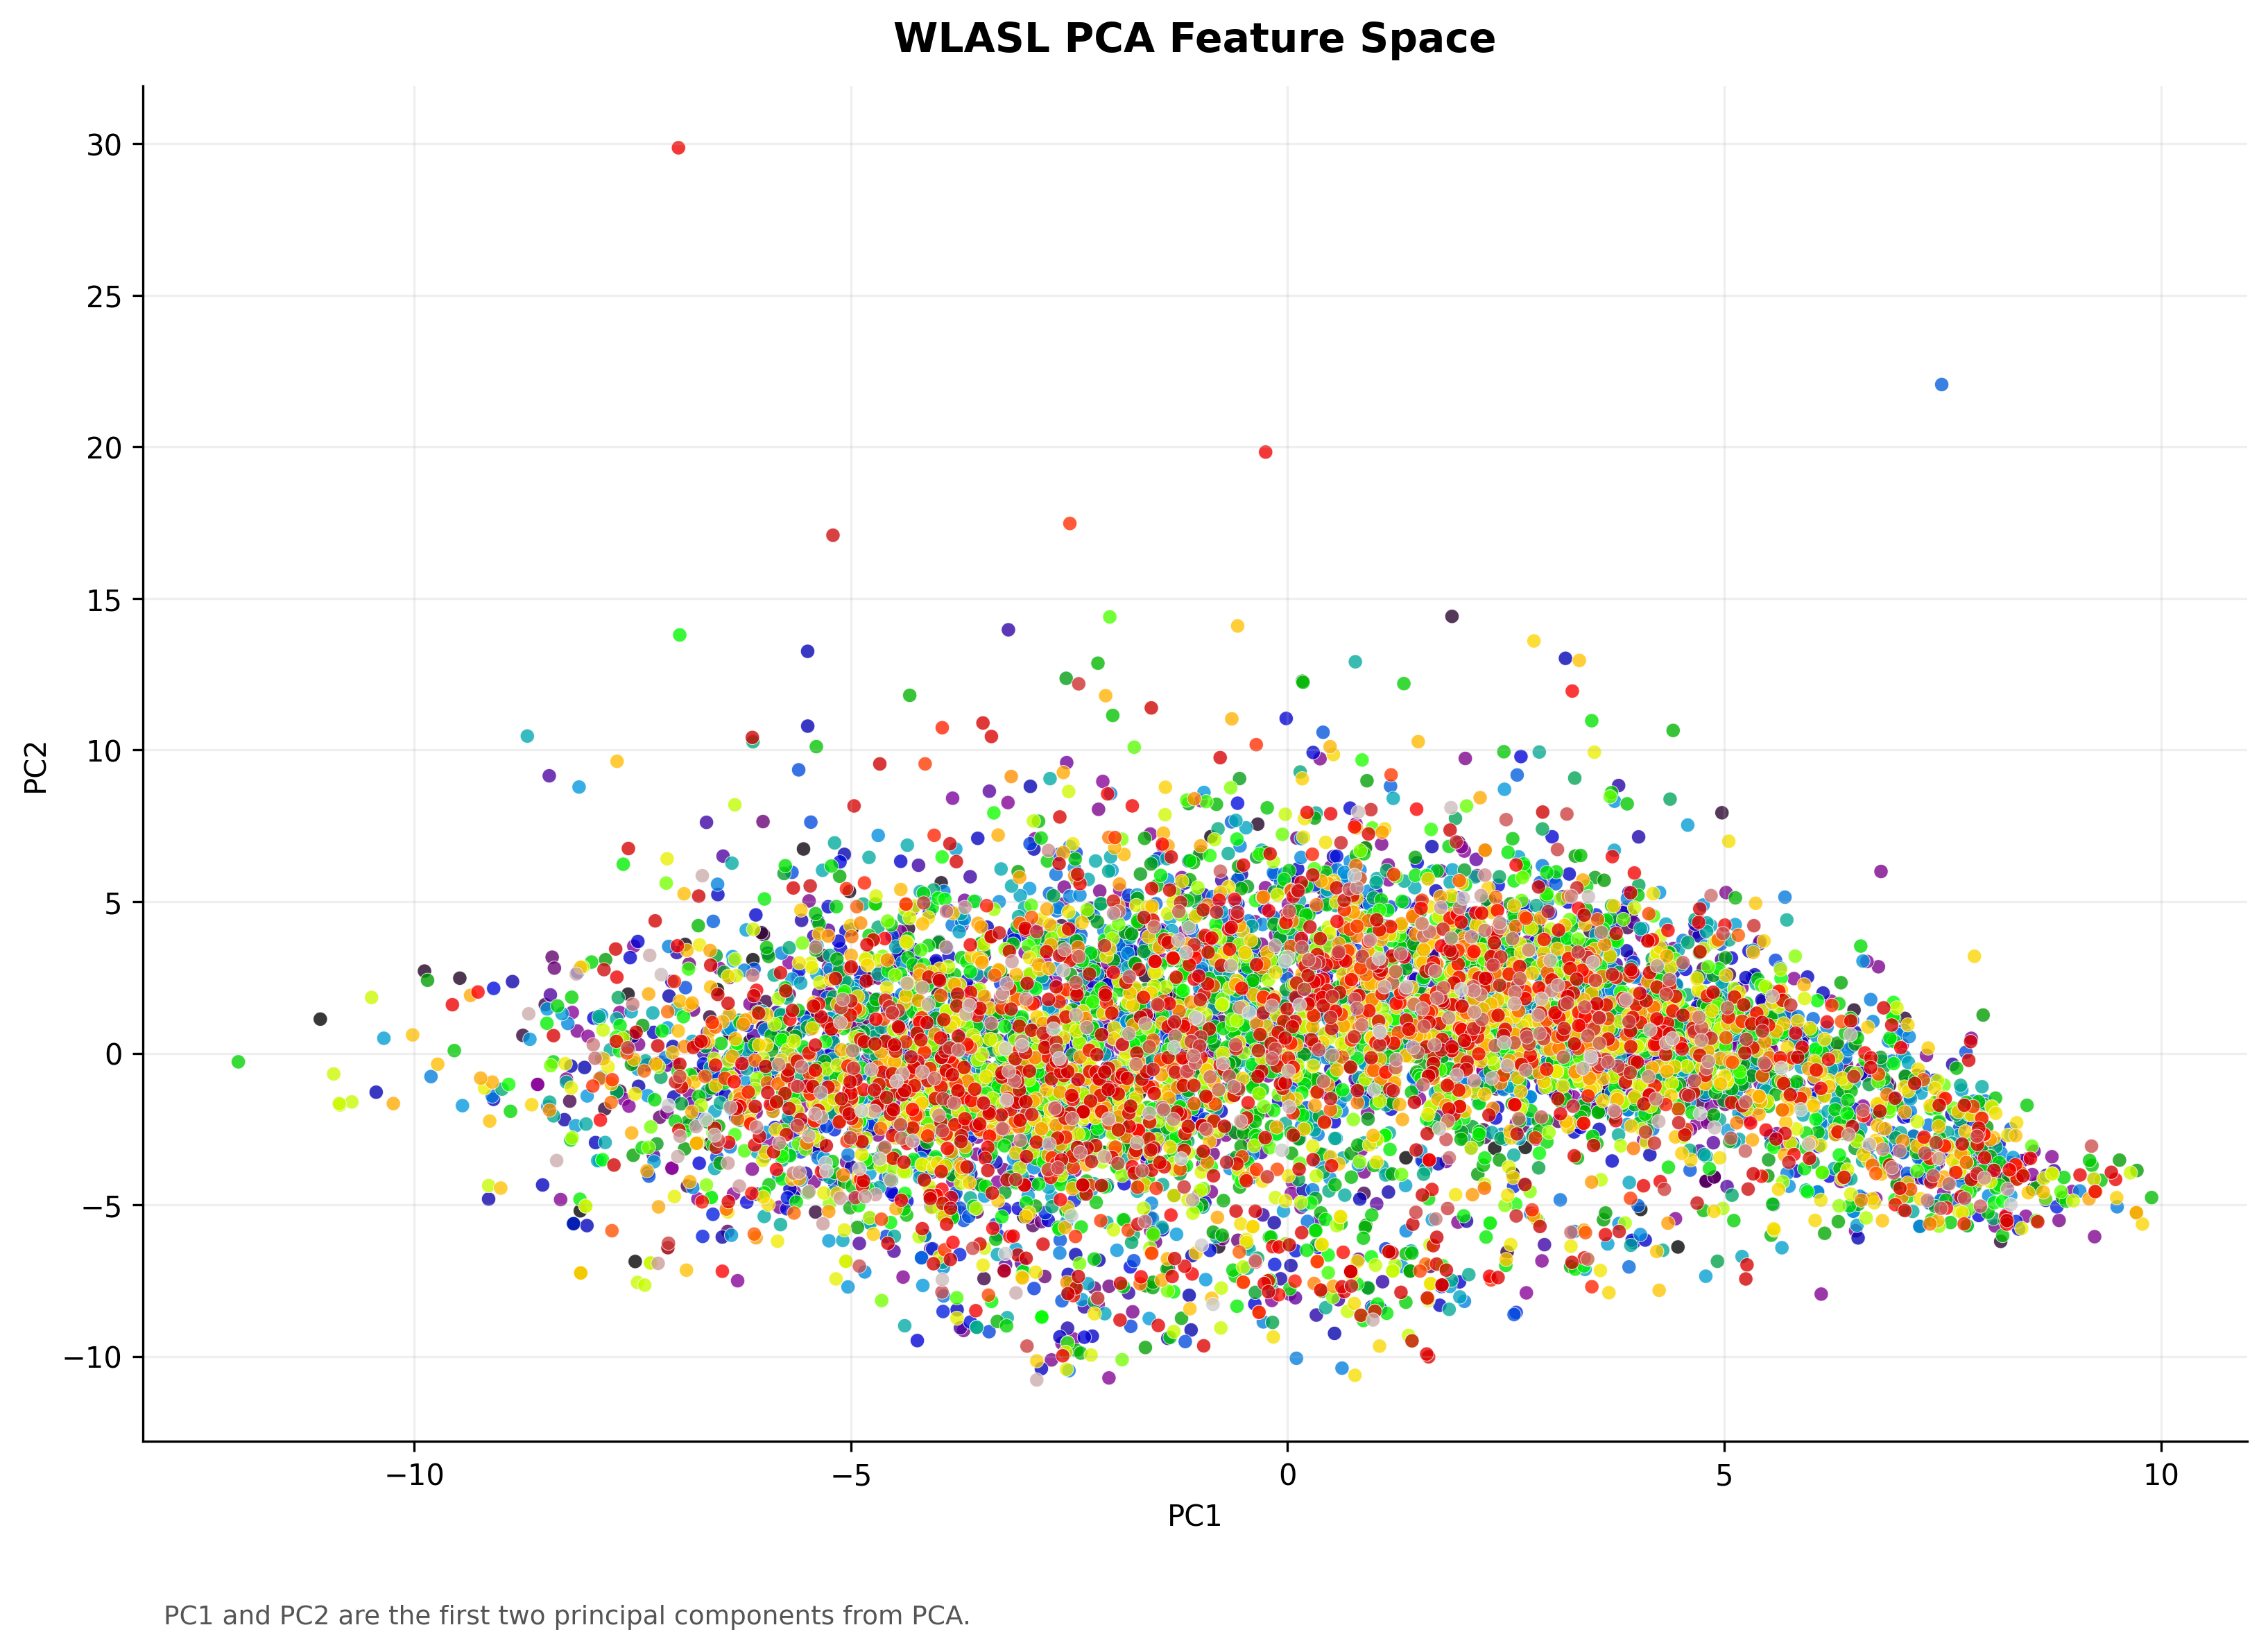
\includegraphics[width=\linewidth]{../ACCESS_latex_template_20260513_V2/figures/wlasl_pca.png}
\caption*{(a) WLASL PCA}
\end{minipage}
\begin{minipage}{0.49\linewidth}
\centering
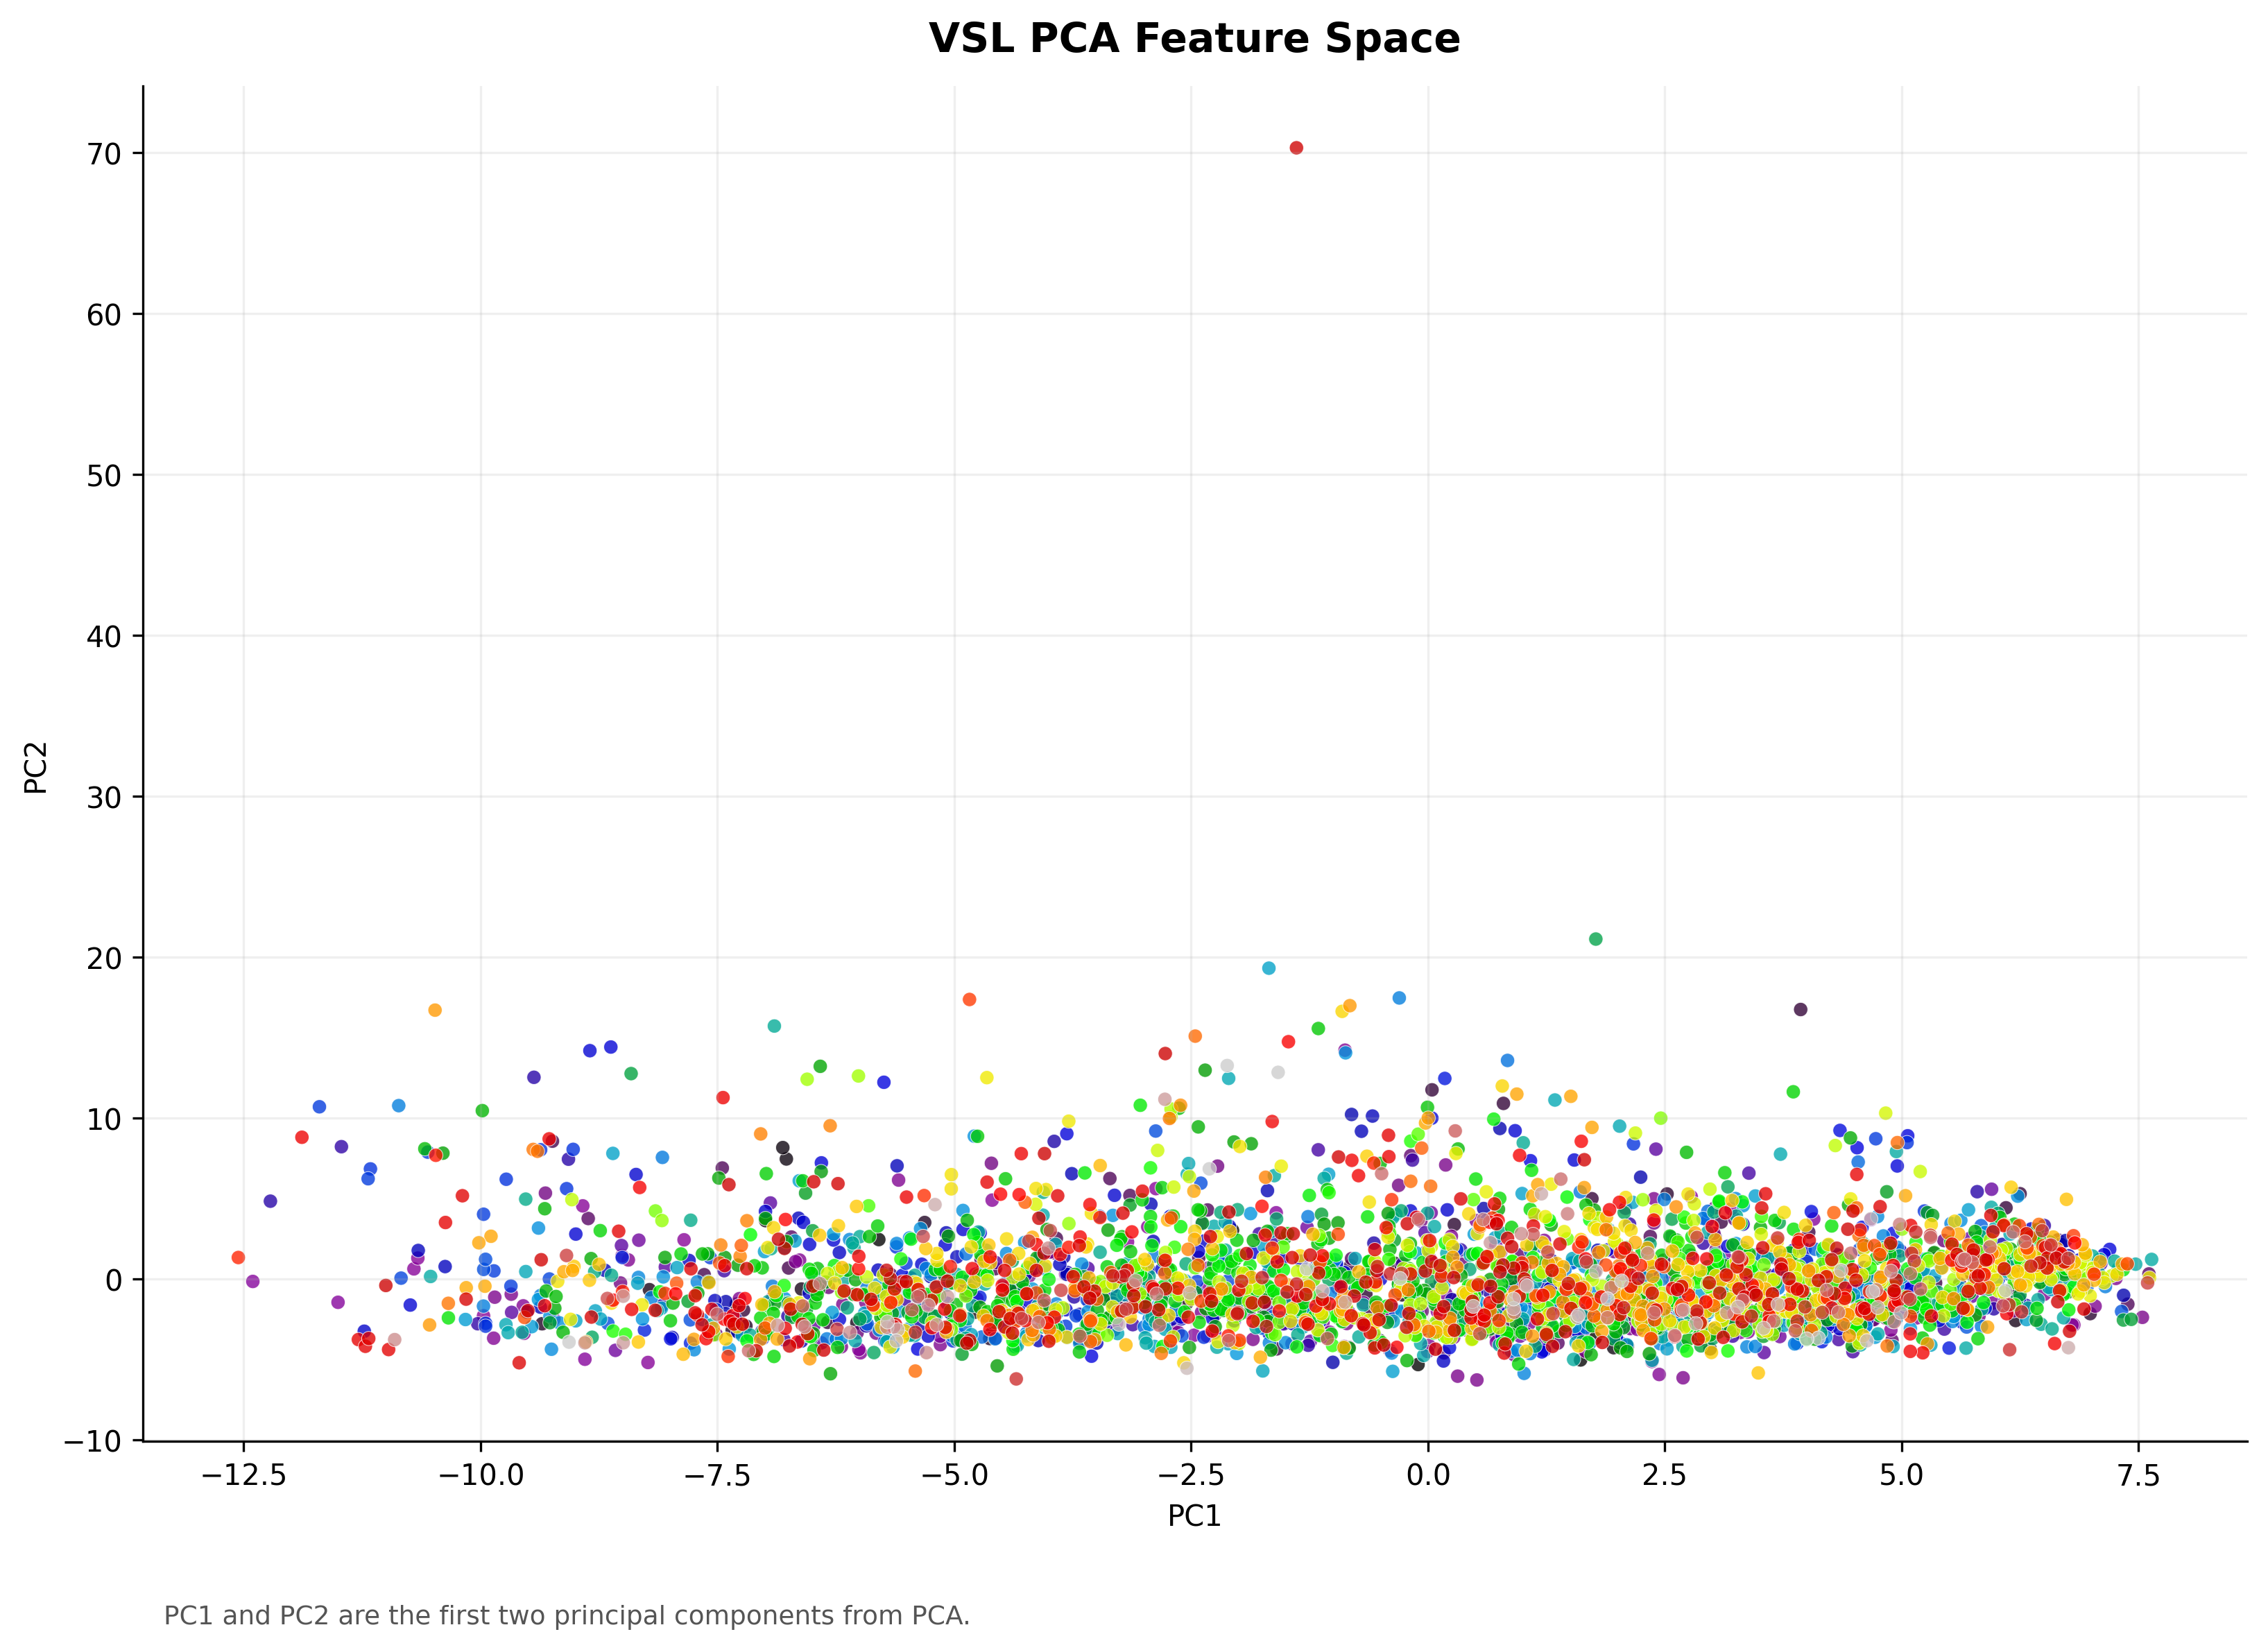
\includegraphics[width=\linewidth]{../ACCESS_latex_template_20260513_V2/figures/vsl_pca.png}
\caption*{(b) VSL PCA}
\end{minipage}
\caption{\textbf{Principal-component projections of the aggregated feature space.} PCA exposes the dominant linear variance directions but does not fully separate gloss neighborhoods, consistent with the moderate explained-variance ratios reported in Table~\ref{tab:feature_space_summary}.}
\label{fig:pca_pair}
\end{figure*}

\begin{figure*}[htbp]
\centering
\begin{minipage}{0.49\linewidth}
\centering
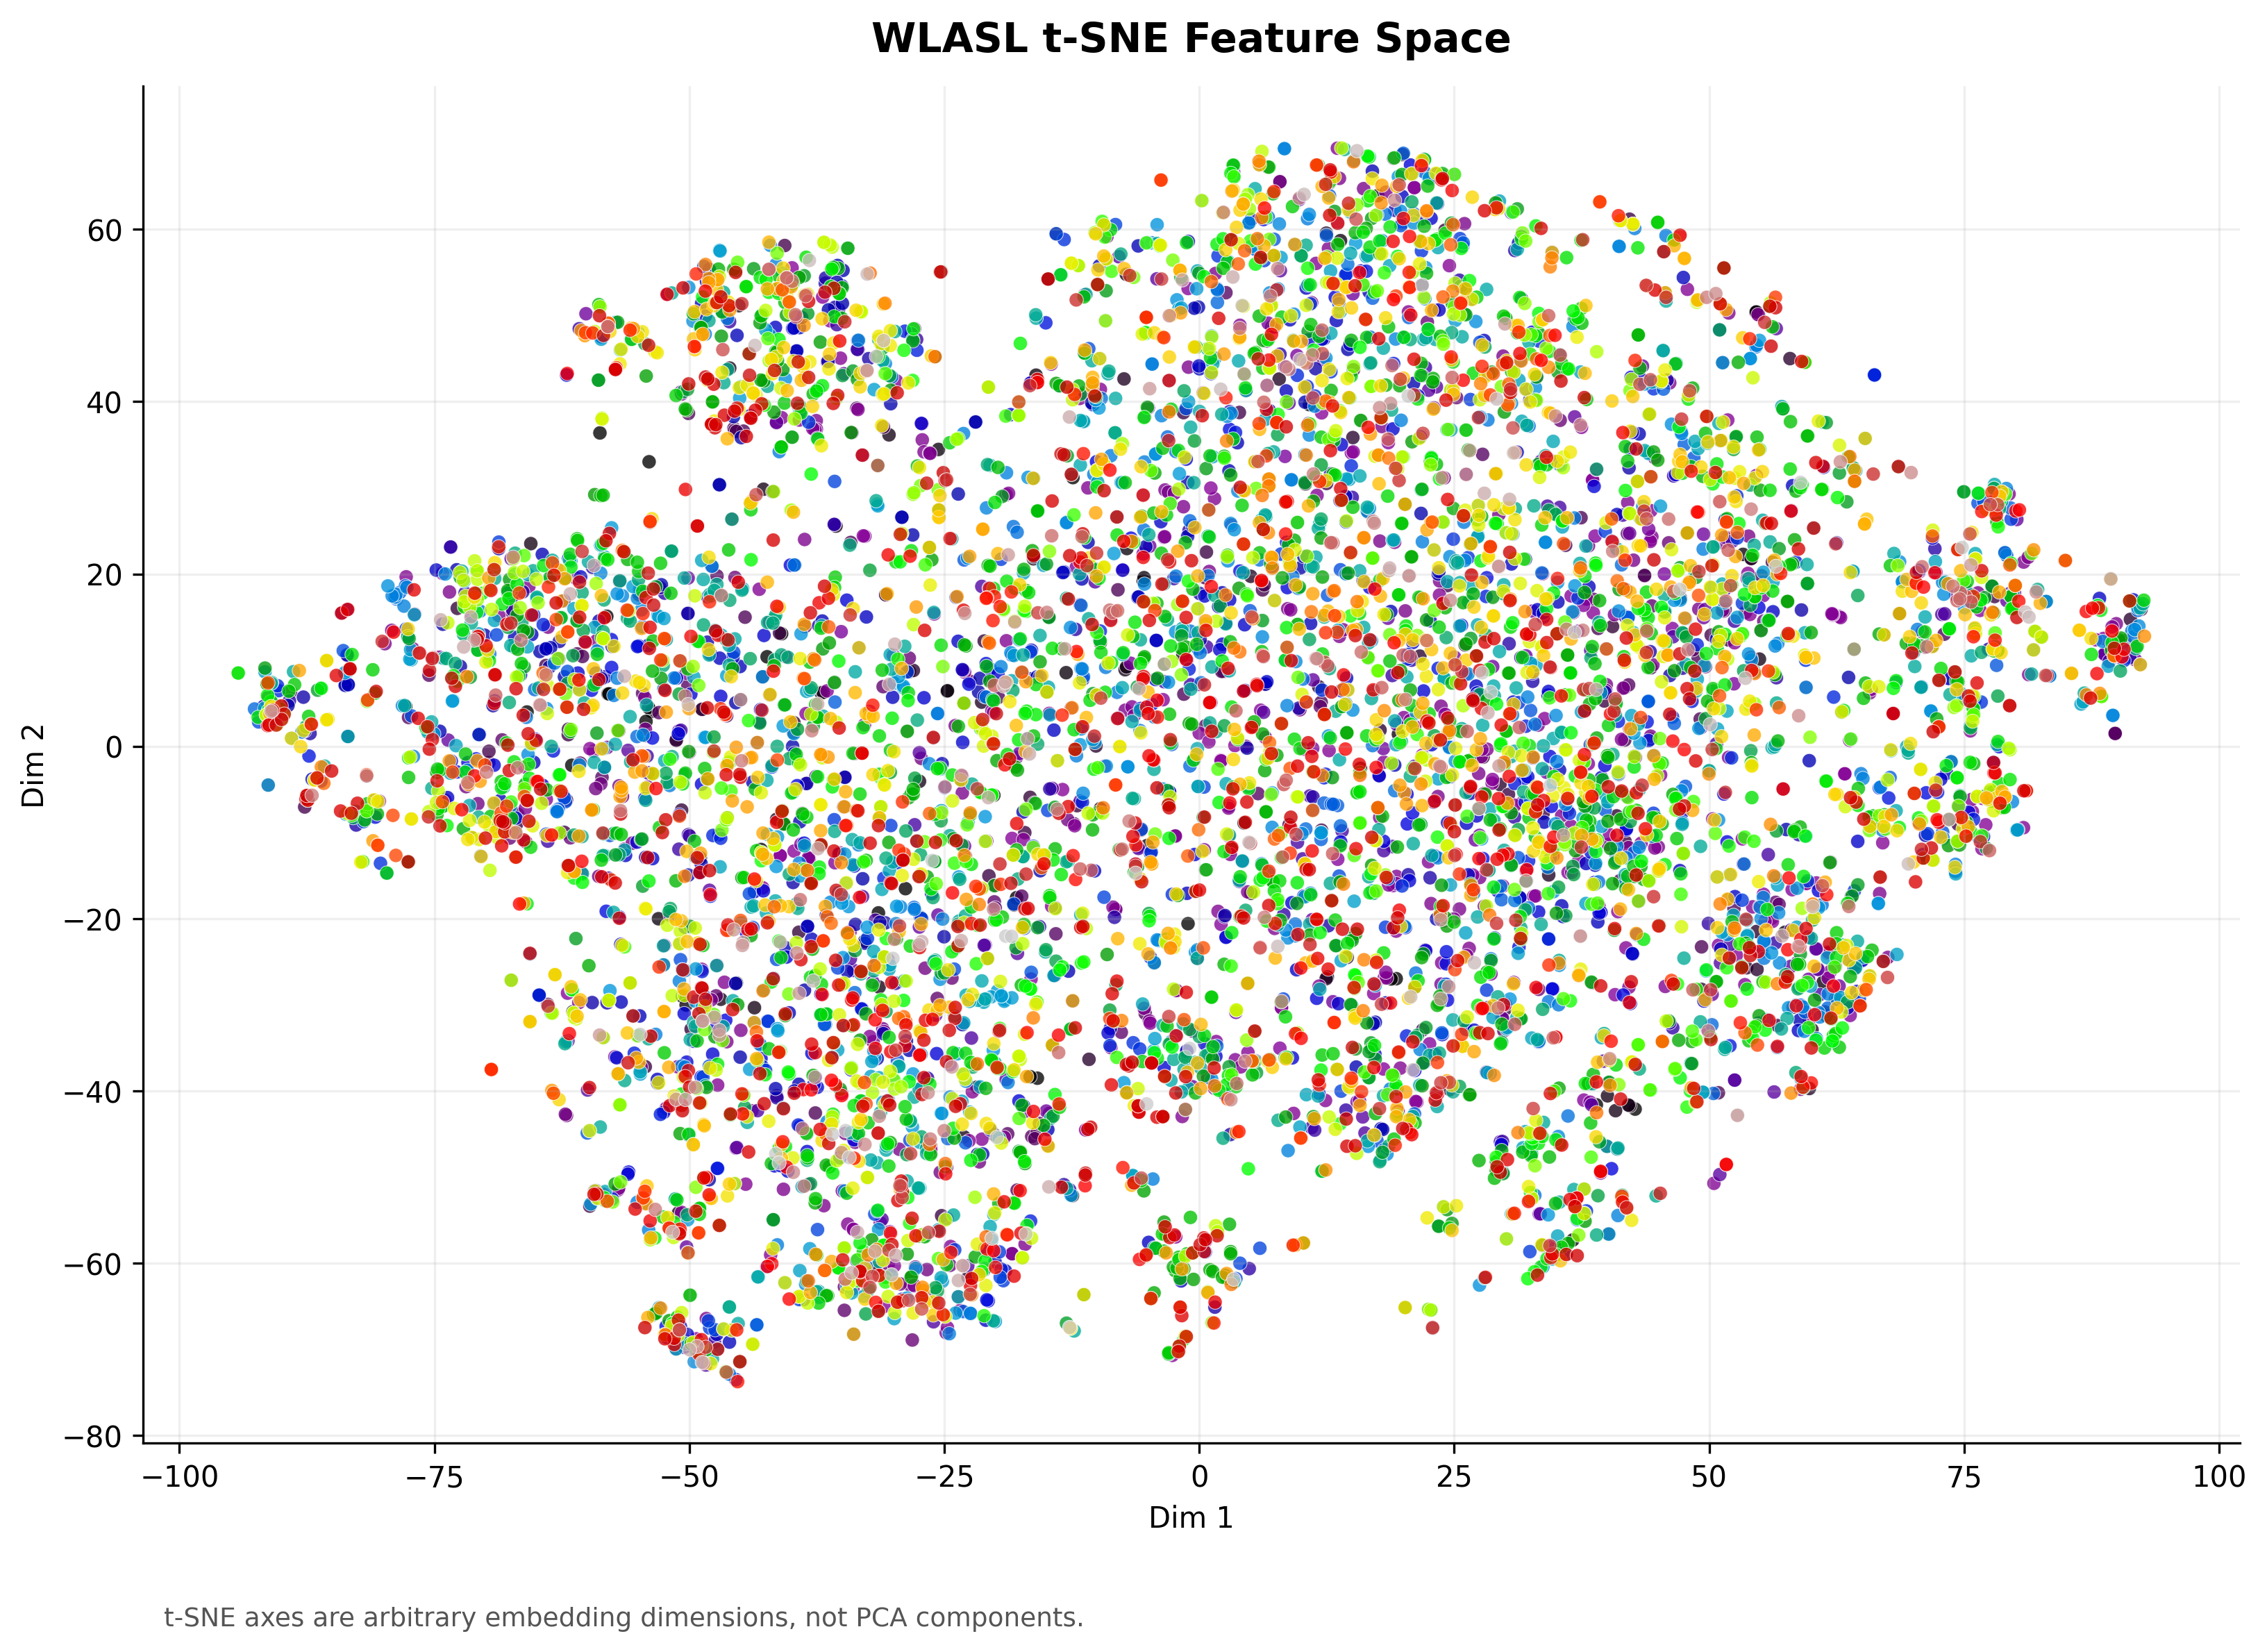
\includegraphics[width=\linewidth]{../ACCESS_latex_template_20260513_V2/figures/wlasl_tsne.png}
\caption*{(a) WLASL t-SNE}
\end{minipage}
\begin{minipage}{0.49\linewidth}
\centering
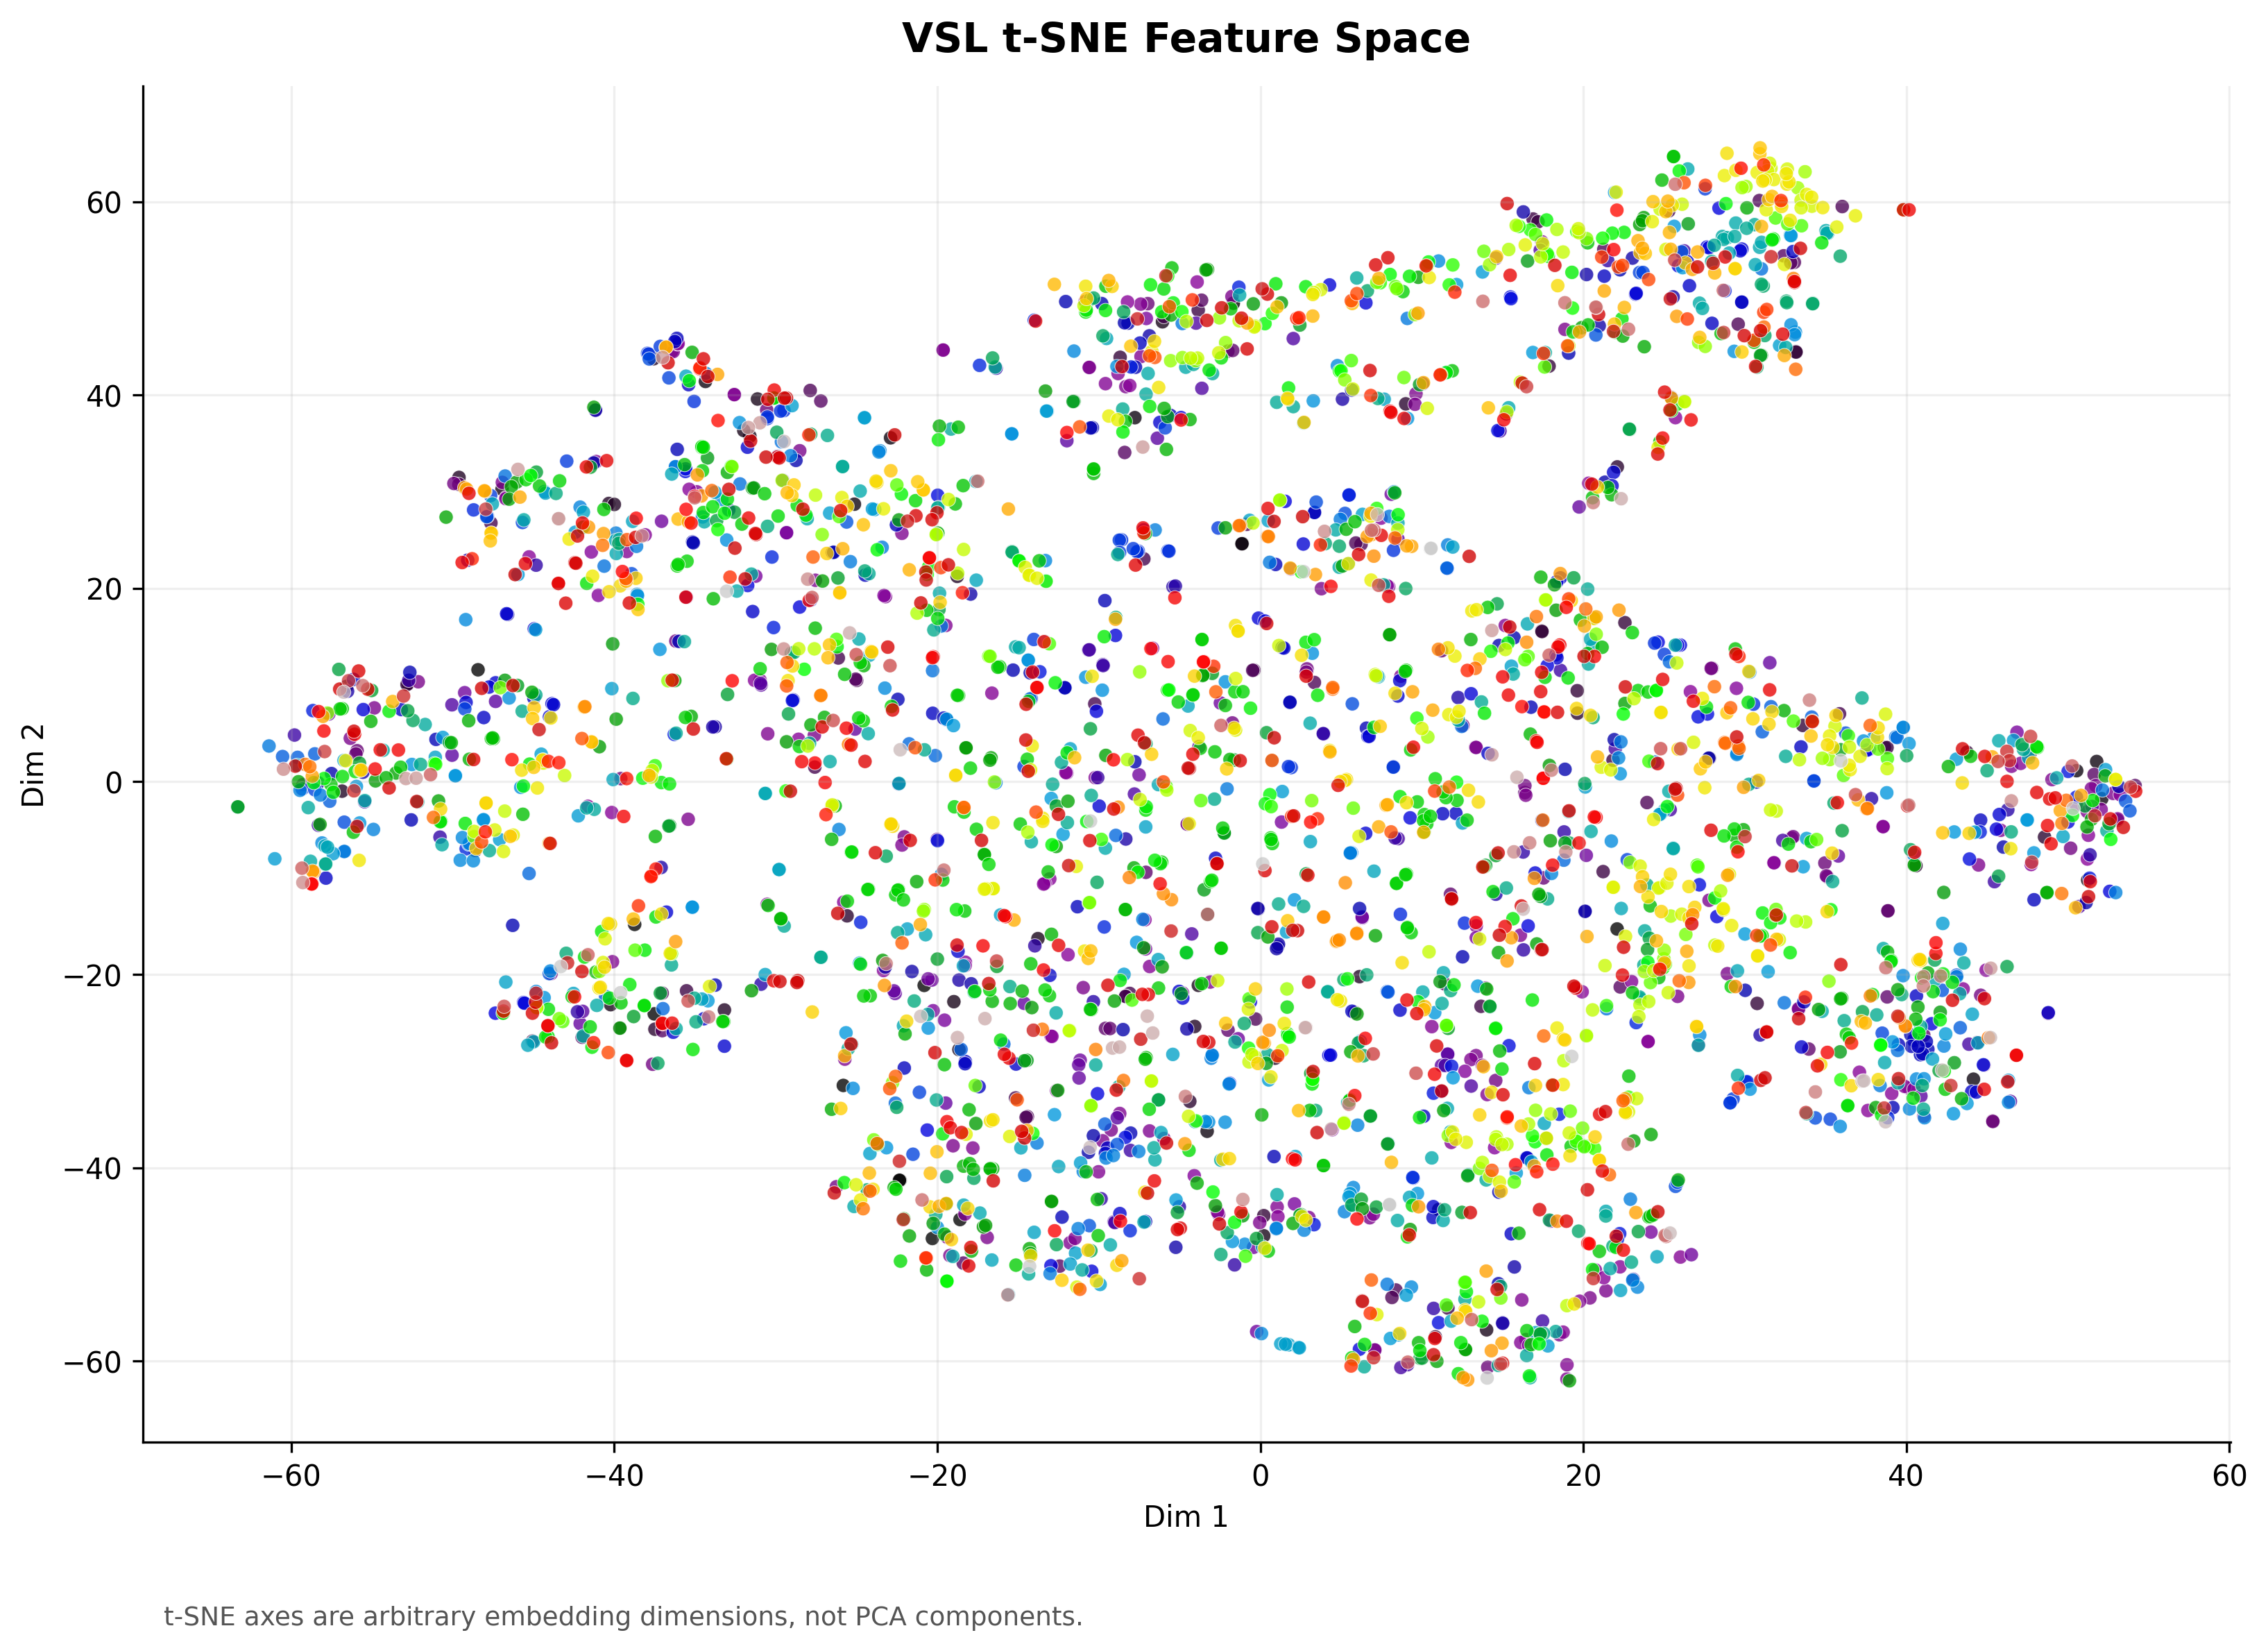
\includegraphics[width=\linewidth]{../ACCESS_latex_template_20260513_V2/figures/vsl_tsne.png}
\caption*{(b) VSL t-SNE}
\end{minipage}
\caption{\textbf{Local-neighborhood structure under t-SNE.} The non-linear embedding reveals multiple dense pockets, bridges, and fragmented regions, indicating that locality is preserved better than global linear separability.}
\label{fig:tsne_pair}
\end{figure*}

\begin{figure*}[htbp]
\centering
\begin{minipage}{0.49\linewidth}
\centering
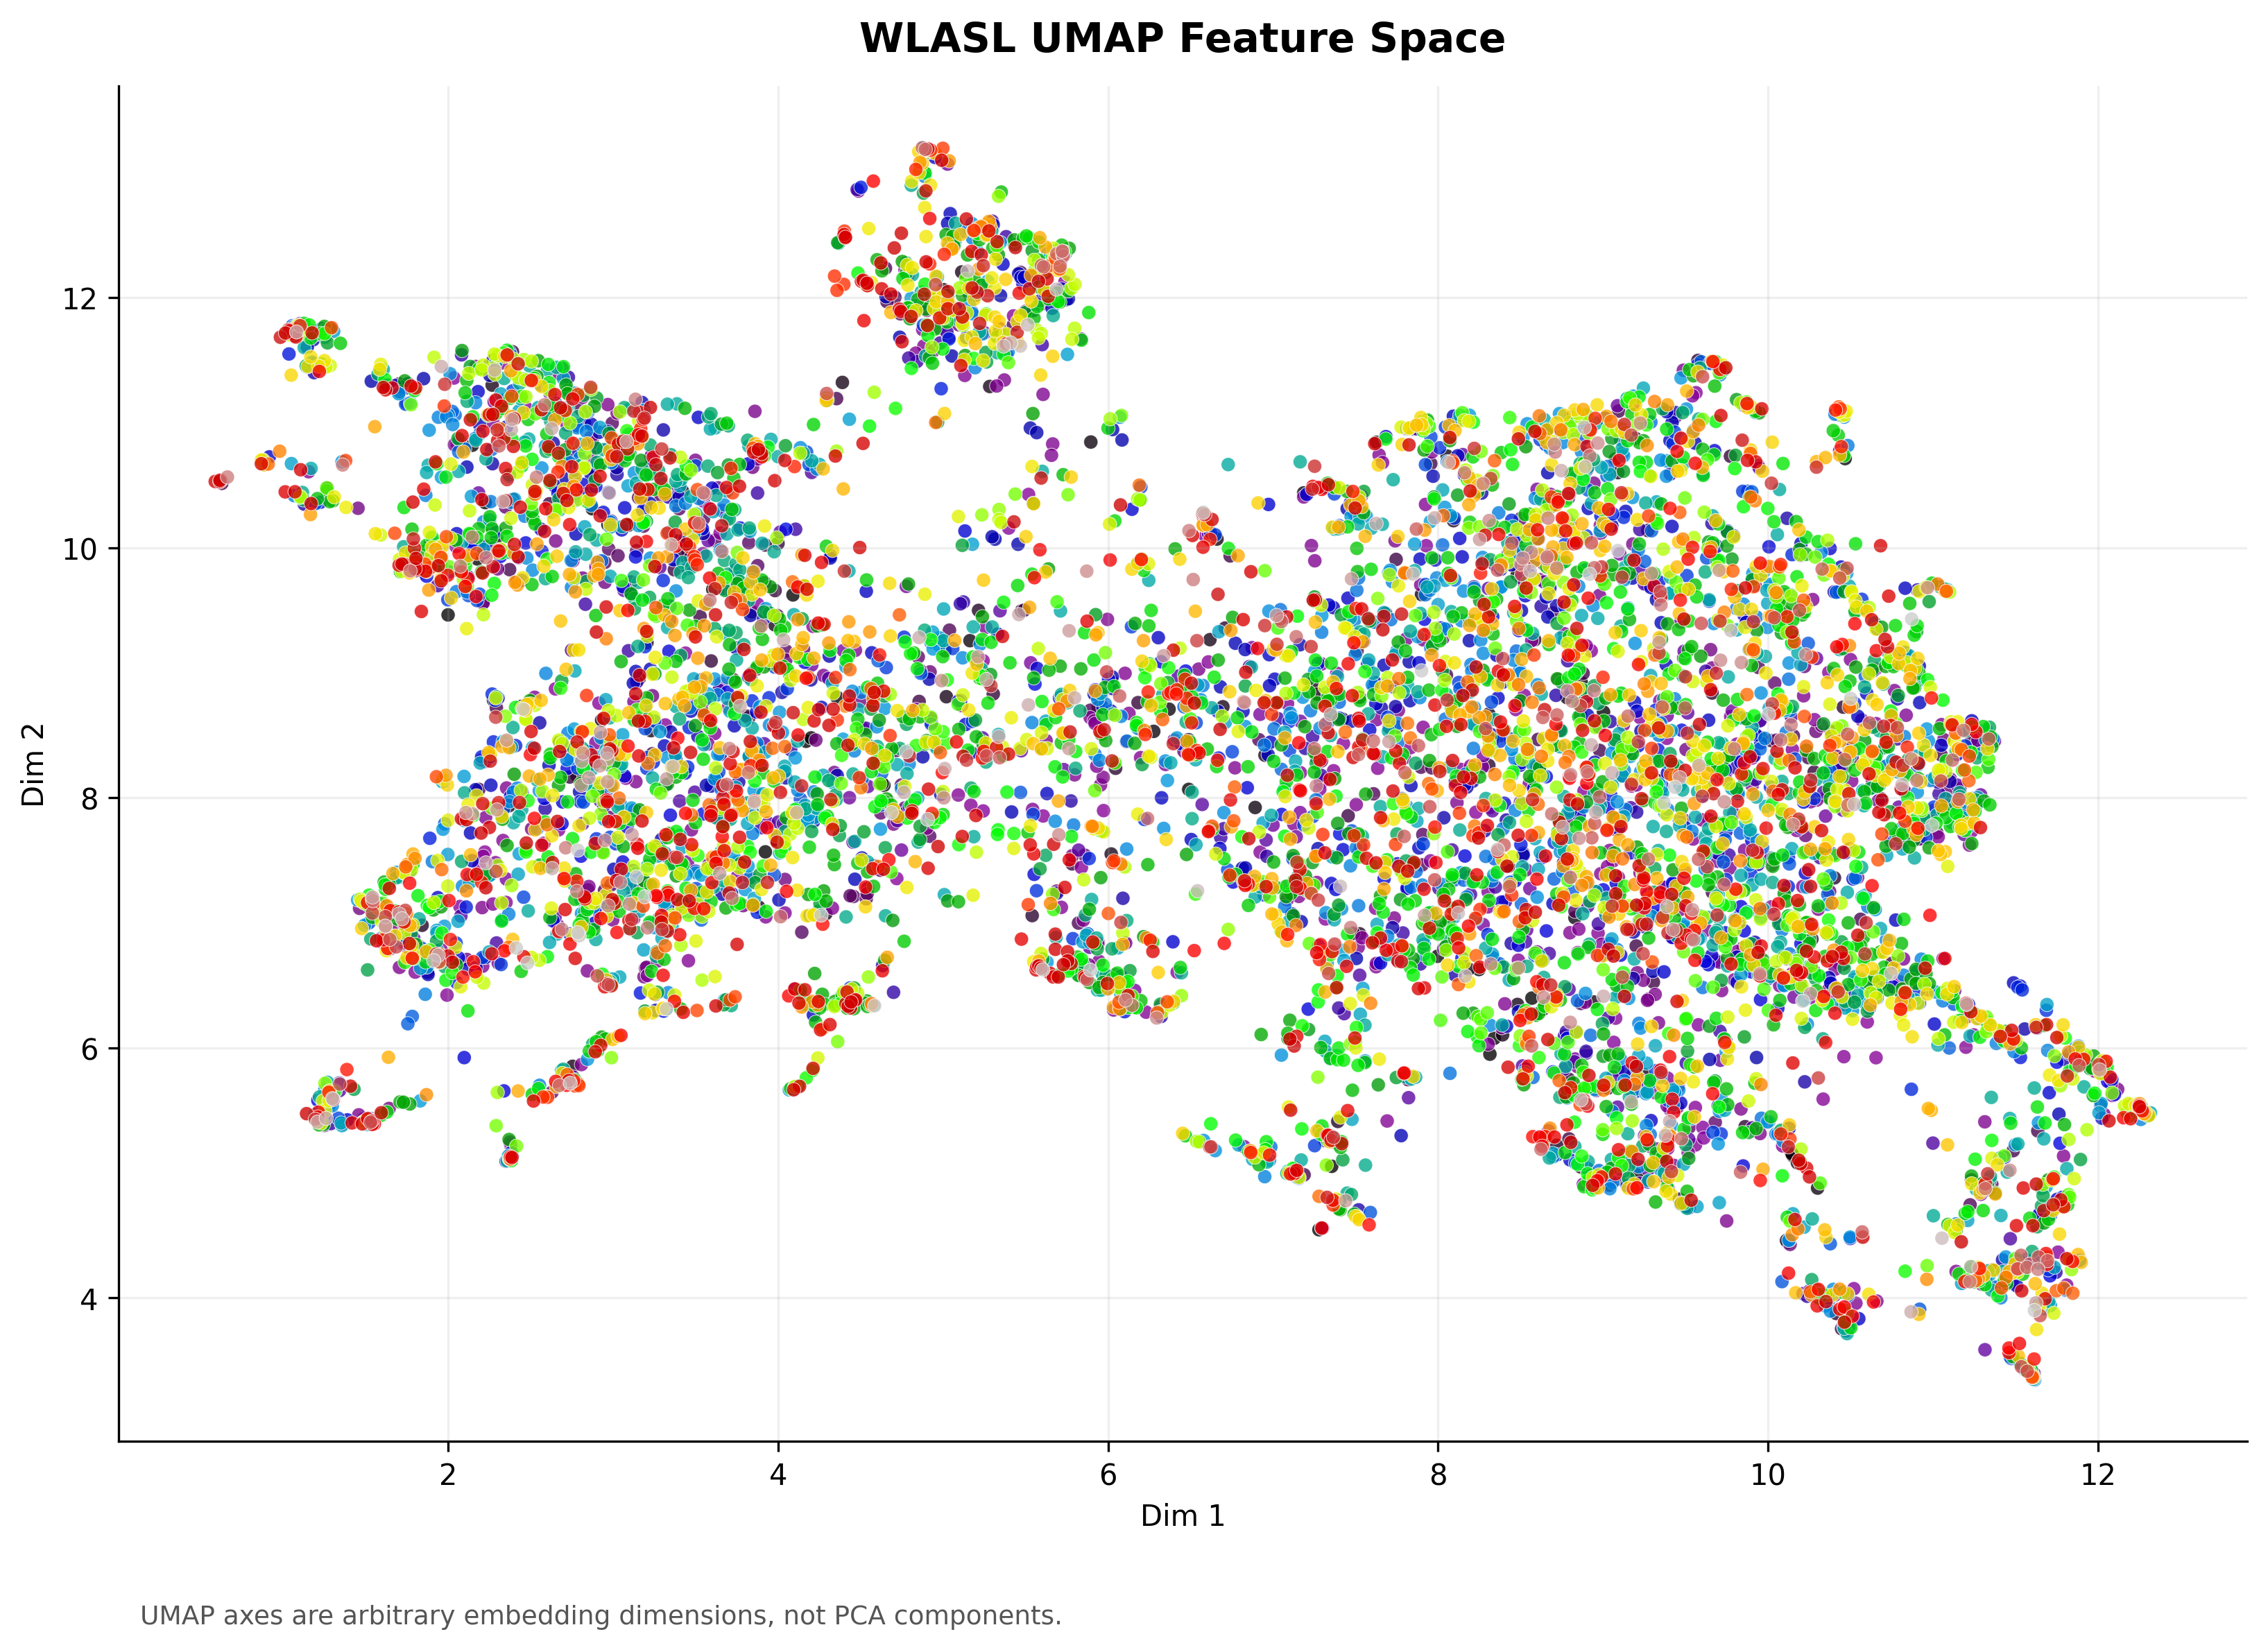
\includegraphics[width=\linewidth]{../ACCESS_latex_template_20260513_V2/figures/wlasl_umap.png}
\caption*{(a) WLASL UMAP}
\end{minipage}
\begin{minipage}{0.49\linewidth}
\centering
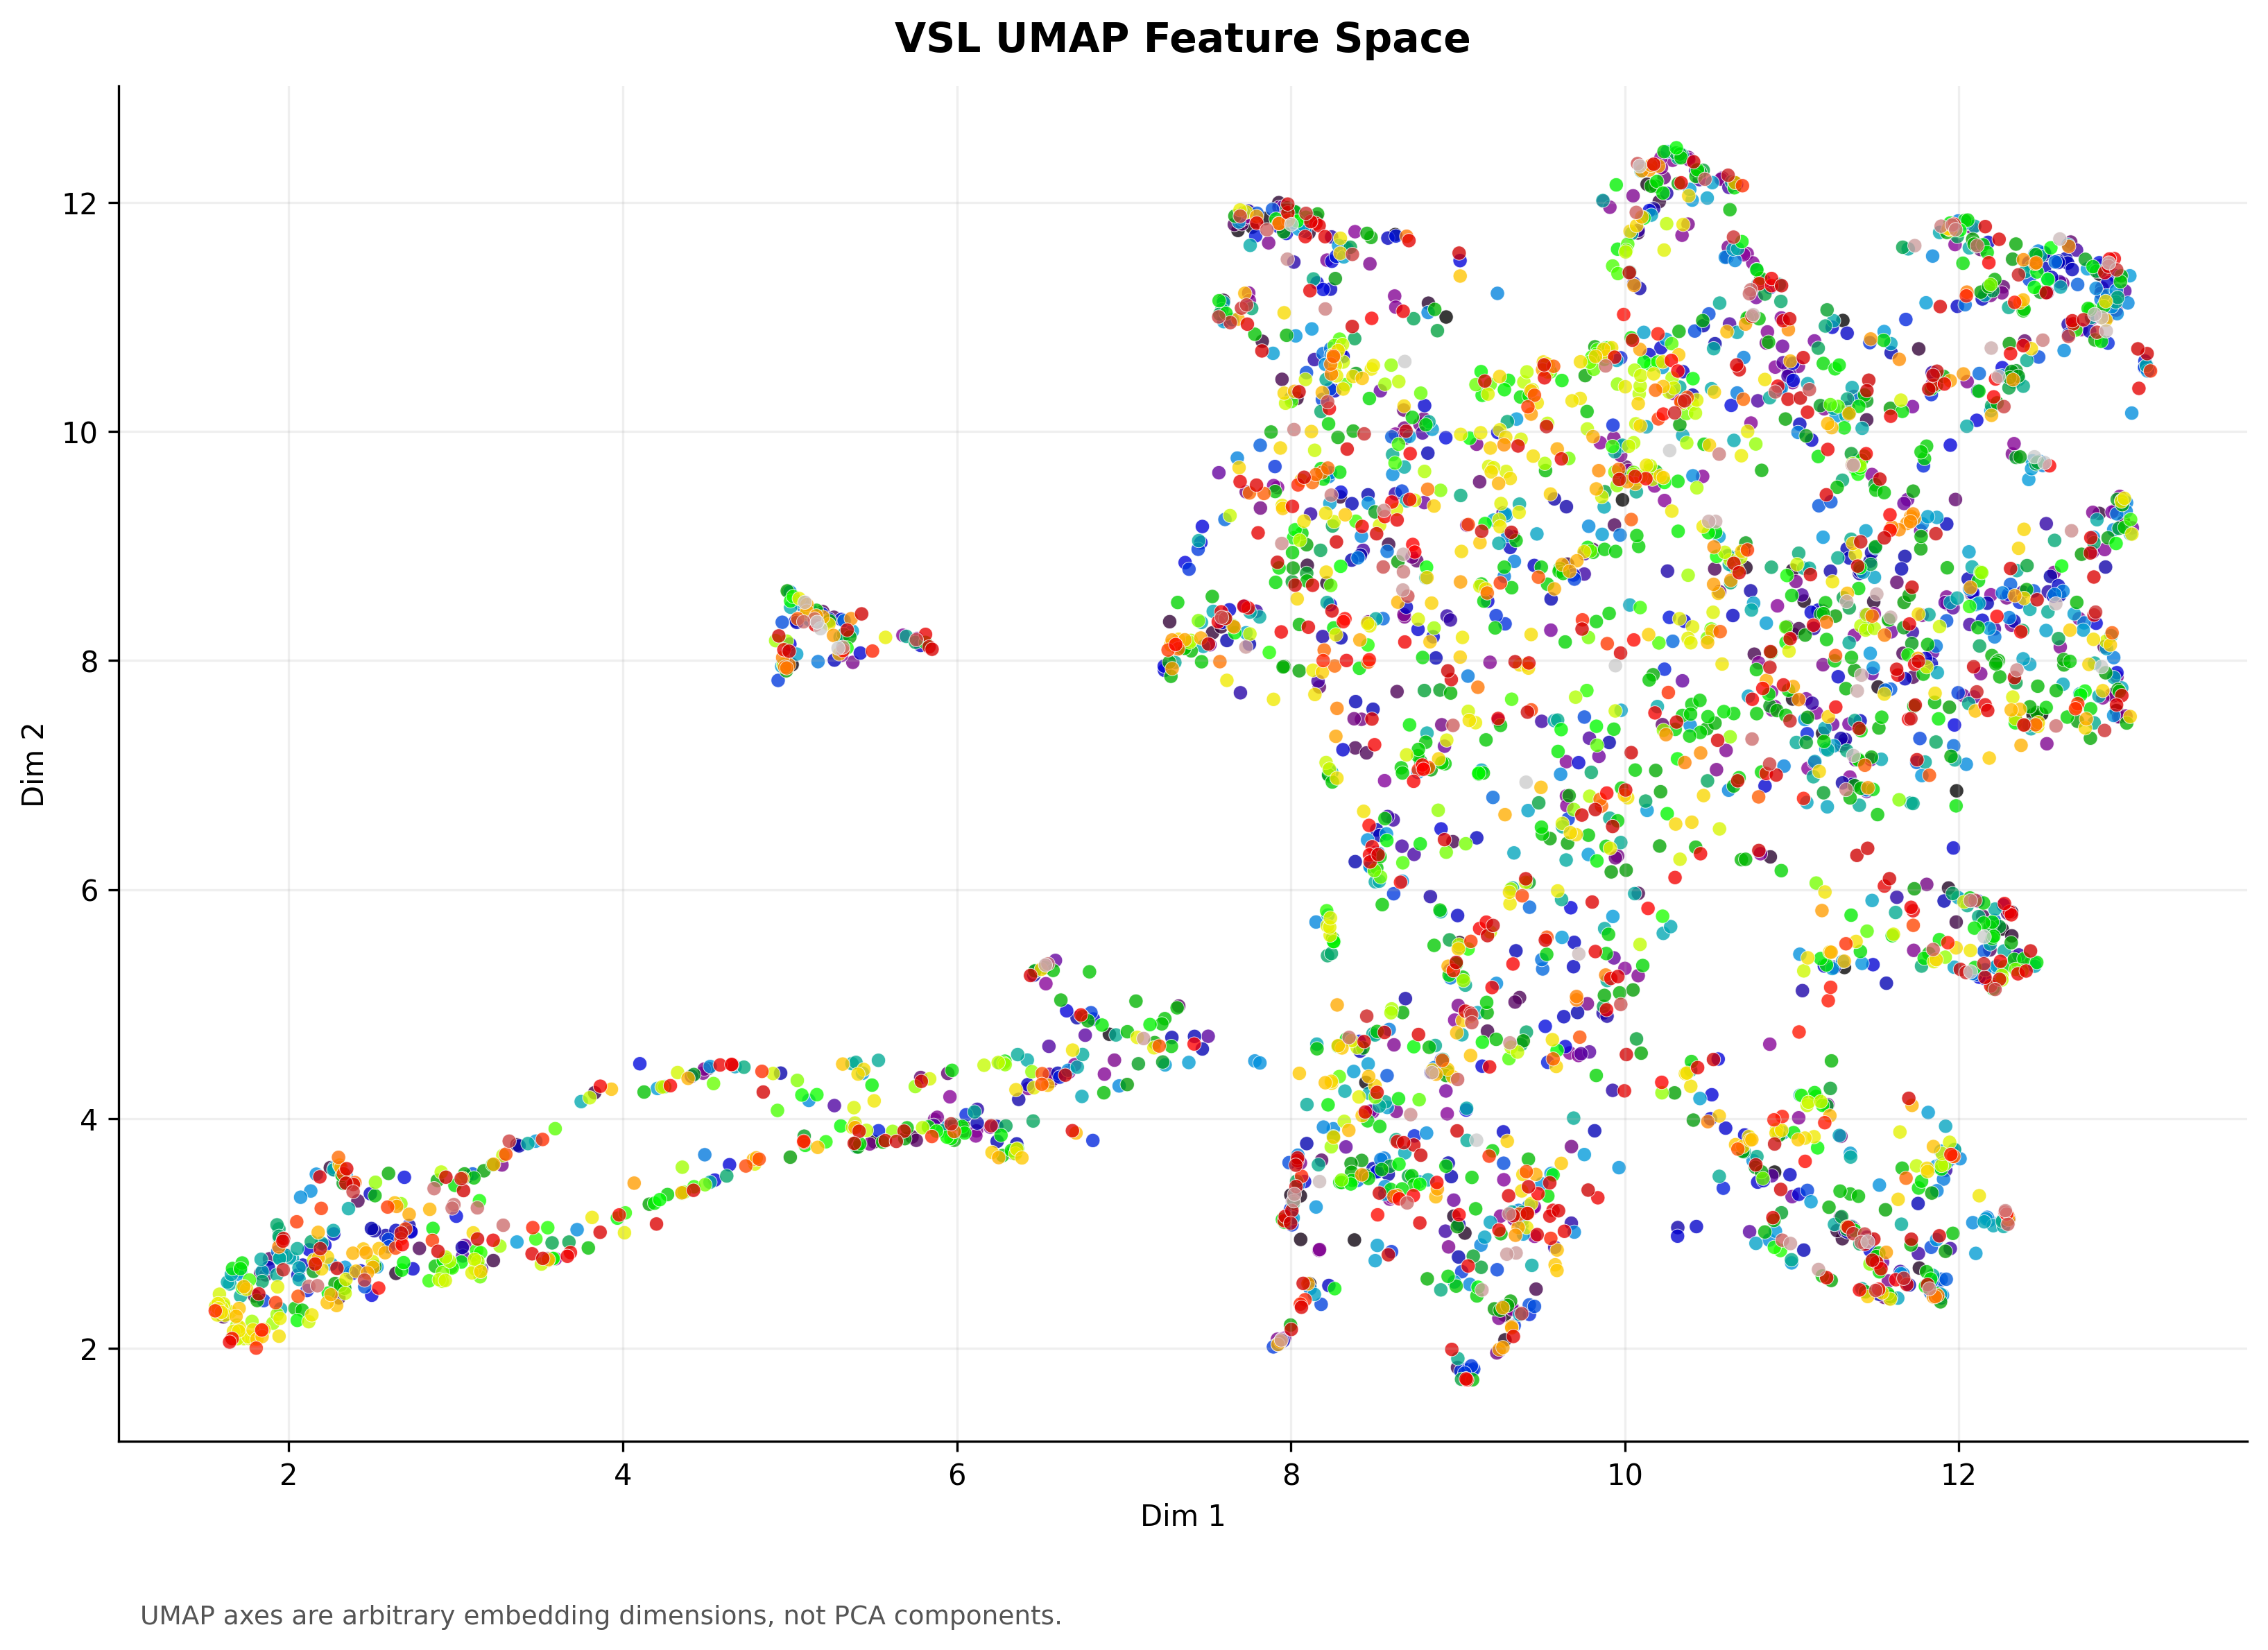
\includegraphics[width=\linewidth]{../ACCESS_latex_template_20260513_V2/figures/vsl_umap.png}
\caption*{(b) VSL UMAP}
\end{minipage}
\caption{\textbf{Manifold organization under UMAP.} UMAP preserves both local neighborhoods and broader manifold continuity, showing that the corpus contains connected semantic regions alongside isolated outliers.}
\label{fig:umap_pair}
\end{figure*}

The visual and numerical evidence should be read together rather than independently. In the PCA views, both corpora form broad overlapping clouds with peripheral outliers, which suggests that the dominant variance directions are shared by multiple glosses rather than cleanly partitioned by class. The t-SNE and UMAP views reveal more structure: local pockets appear within each corpus, but the pockets are connected by bridges and interleaved with nearby classes. This is consistent with the geometry one would expect when the descriptor space captures meaningful articulatory structure but the sample density is too low to resolve sharp class boundaries. In other words, the representations are informative, yet not sufficiently compressed into separable islands for naive linear discrimination.

The cluster scores reinforce that interpretation. A negative Silhouette Score indicates that many samples are, on average, not closer to their own class neighborhood than to neighboring classes. The Davies--Bouldin Index points to the same phenomenon from the opposite angle: when scatter is high relative to inter-centroid distance, cluster boundaries remain unstable. The compactness outputs add an important caveat for the VSL corpus. Singleton glosses yield zero within-class spread by construction, so a zero median compactness does not imply a genuinely tight manifold; it reflects the extreme sparsity documented earlier in the paper. The same caution applies to Euclidean and cosine separation. Large inter-class distances and low cosine similarity identify strongly dissimilar pairs, but they do not tell us whether those pairs are representative of the corpus as a whole or simply reflect a few semantically distant, high-motion outliers.

To make that distinction concrete, the cross-lingual similarity analysis in Section~\ref{sec:similarity} shows that some pairs are almost isomorphic in the descriptor space while others differ strongly in handshape, movement, and orientation. The mean cosine similarity of 0.5701 and the wide range from 0.1505 to 0.9742 indicate that transferability is heterogeneous, not binary. Highly iconic pairs such as ``bụng''--``abdomen'' occupy a shared neighborhood, whereas culturally specific signs such as ``phòng thư viện''--``library'' remain far apart. This pattern is scientifically important because it implies that hard-negative mining should be driven by measured geometric proximity rather than by lexical intuition alone. It also suggests that a single global embedding space may be too coarse for all glosses; some subregions are naturally aligned across languages, while others require explicit adaptation.

The discussion above is best interpreted as a statement about dataset geometry, not about recognition accuracy. The analyses do not train a classifier and do not measure downstream recognition performance. What they do show is that representation learning will have to contend with three interacting sources of difficulty: sparse within-class sampling, non-linear manifold folding, and cross-lingual neighborhoods that are sometimes close and sometimes sharply separated. That combination explains why missingness-aware masking, temporal normalization, and contrastive objectives are scientifically justified for low-resource sign-language corpora \cite{buda2018systematic, chen2020simple, robinson2020contrastive, sakoe1978dynamic}.

% Revised: Ensured IEEE Access section formatting and preserved the critical transition paragraph.
\section{Proposed Domain-Aware Training Blueprint} \label{sec:actionplan}

Taken together, these sparsity metrics, the 30\%+ MediaPipe failure rates, the 2.07 $\times$ higher motion amplitudes, and the substantial inter-signer variation suggest that conventional supervised training architectures may face challenges in real-world, grassroots SLR deployment. To address this gap, the study moves from empirical observation to structural algorithmic reform. 

We formulate a comprehensive, domain-aware training blueprint specifically designed to mitigate the vulnerabilities identified in our analysis. We hypothesize that models may benefit from shifting from standard Softmax classification to hard-negative contrastive metric learning \cite{chen2020simple}, \cite{robinson2020contrastive}, utilizing explicitly computed DTW distances to separate overlapping topologies. Furthermore, architectural components should incorporate missing-landmark masking and adaptive temporal bucketing to better handle the erratic nature of VSL.

To transition from theoretical diagnostics to practical architectural implementation, we propose a domain-aware training blueprint specifically adapted to the vulnerabilities mapped in the previous sections. Table \ref{tab:action_plan} synthesizes our empirical findings into a formalized 5-step action plan designed to address the extreme sparsity, motion tracking failures, and domain shifts inherent in grassroots datasets.

\begin{table*}[!t]
\caption{Proposed Five-Step Domain-Aware Training Blueprint for Low-Resource Cross-Lingual Sign Language Recognition}
\label{tab:action_plan}

\centering
\small
\setlength{\tabcolsep}{5pt}

\begin{tabular}{p{0.7cm}p{3.2cm}p{11.8cm}}

\toprule

\textbf{Step} &
\textbf{Training Stage} &
\textbf{Recommended Strategy} \\

\midrule

1 &
Data Quality Assessment &
Identify recordings exhibiting severe hand-landmark missingness rather than discarding them. Preserve reliable face and body landmarks while explicitly masking missing hand features to reduce feature corruption and maximize data utilization. \\

\addlinespace

2 &
Dataset Stratification &
Partition the corpus according to class frequency. Train supervised classifiers using sufficiently populated classes (e.g., $n\ge3$ or $n\ge5$), while reserving singleton and extremely sparse classes for few-shot or retrieval-based evaluation. \\

\addlinespace

3 &
Backbone Architecture &
Adopt a Transformer or Temporal Convolutional Network (TCN) incorporating temporal attention masks, explicit landmark-missing masks, relative spatial encoding, and adaptive sequence padding to accommodate variable-length signing sequences. \\

\addlinespace

4 &
Contrastive Representation Learning &
Incorporate DTW-based hard-negative mining into the training objective to distinguish visually similar trajectories that differ primarily in handshape, orientation, or articulation dynamics. \\

\addlinespace

5 &
Robustness Evaluation &
Evaluate ASL and VSL independently and additionally report performance across low-, medium-, and high-missingness groups, as well as on a dedicated hard-label benchmark comprising highly complex signs with large motion amplitudes, substantial sequence-length variance, and low cross-lingual similarity. \\

\bottomrule

\end{tabular}

\vspace{2mm}

\footnotesize
\textit{Note:}
The proposed training blueprint is derived from the empirical observations presented throughout this study, including severe class imbalance, high temporal variability, frequent landmark missingness, and substantial cross-lingual kinematic divergence between the VSL and WLASL corpora.

\end{table*}

This blueprint is deliberately ordered: Steps 1--2 address data quality and sampling structure before any model is trained; Step 3 encodes the kinematic and missingness findings directly into the architecture; Step 4 uses the confusability structure as a targeted training signal; and Step 5 ensures that the documented variance and imbalance effects remain visible in reported results rather than being averaged out in top-level accuracy metrics.

\section{Discussion and Limitations} \label{sec:discussion}

The analyses in this paper converge on a single scientific point: the limiting factor in low-resource sign-language recognition is not only model capacity, but the geometry of the dataset itself. Long-tail sparsity, variable sequence length, inter-signer diversity, and missing landmark observations jointly define the empirical landscape in which any recognizer must operate. Densely sampled corpora such as WLASL provide a more stable sampling manifold, whereas the VSL corpus behaves like a floor-dominated regime in which many glosses are represented by one or a few recordings. In the context of empirical risk minimization, that regime weakens the statistical support for class-conditional invariants and increases the likelihood that optimization will focus on signer-specific or recording-specific nuisance factors \cite{buda2018systematic}.

This interpretation is reinforced by the kinematic analyses. High total motion, elevated velocity, and low straightness ratio are not merely descriptive properties; they change the effective signal-to-noise ratio of the extracted landmarks. When motion becomes more abrupt, holistic trackers are more likely to lose hand observations, and the resulting gaps are not random missing values but structured failures correlated with articulation complexity \cite{lugaresi2019mediapipe}. In that sense, missingness is itself part of the data-generating process. Standard zero-padding is therefore analytically undesirable because it introduces artificial discontinuities into the temporal graph. A more defensible approach is to preserve reliable body and face cues while explicitly masking unreliable hand segments, so that the model learns from observed structure rather than from imputed artifacts.

Cross-lingual DTW adds an additional layer of interpretation. The wide similarity range shows that semantic correspondence is heterogeneous: some pairs are nearly congruent in motion and handshape, whereas others diverge sharply in one or more kinematic subspaces. This matters because the cross-lingual map is not simply a bilingual lexicon; it is a ranked confusability space. Pairs with high similarity are useful anchors for transfer learning, whereas pairs with low similarity are better treated as hard negatives for contrastive objectives \cite{chen2020simple, robinson2020contrastive}. The practical implication is that dataset construction and model training should be aligned: glosses that are dense, stable, and semantically redundant can support standard supervised learning, but sparse and geometrically isolated glosses are better handled with retrieval, metric learning, or explicit augmentation.

The main limitation of the present evidence is scope. The current study characterizes dataset geometry, but it does not measure recognition accuracy under controlled training protocols. As a result, the findings should be interpreted as constraints on representation learning rather than as direct performance predictions. Another limitation is the reliance on monocular 3D pose estimation, which remains vulnerable to self-occlusion, camera angle, and fast motion. A final limitation is the manual nature of the cross-lingual alignment subset, which is necessarily incomplete and may overrepresent visually intuitive pairs while underrepresenting culturally complex mappings. These limitations do not invalidate the core conclusion, but they do restrict the scope of the evidence to descriptive and geometric analysis.

Taken together, the corpus properties identified here motivate a domain-aware training strategy: preserve missingness information, stratify by class support, exploit DTW-based hard negatives, and evaluate low-resource classes separately from dense ones. This is a methodological implication of the data, not a claim about any specific model's achieved accuracy. It represents a principled route toward reducing the mismatch between the geometry of sign-language corpora and the assumptions embedded in conventional supervised pipelines.

\section{Conclusion} \label{sec:conclusion}

This study presented a large-scale structural, kinematic, and semantic comparative analysis of 16,342 video sequences, characterizing the domain shift between high-resource algorithmic benchmarks (WLASL) and low-resource, grassroots corpora (custom VSL). Our empirical investigation characterizes the data conditions that currently limit cross-lingual transfer learning. We demonstrated that real-world VSL data is constrained by a floor-dominated long-tail imbalance, yielding a severe Gini coefficient of 0.203 and an average of 1.32 samples per class, contrasting sharply with the 5.99 average of the WLASL baseline. Kinematically, VSL execution is associated with notably longer temporal sequences (92.48 mean frames), generates a 2.07 $\times$ higher total motion amplitude, and produces highly recursive, curved spatial trajectories (straightness ratio of 0.039) compared to ASL. Furthermore, our topological analysis revealed a heavy skew toward two-handed execution in VSL (72.8\%) relative to ASL (64.7\%), which intrinsically multiplies the probability of intersecting feature trajectories and spatial occlusion. 

The practical implications of these structural divergences suggest a shift in how spatial-temporal models are engineered for low-resource deployment. The combined effects of high execution velocity and severe trajectory curvature are associated with substantial hand-landmark missing rates, which we observed to reach 39.6\% in ASL and 32.3\% in VSL. Consequently, the standard programmatic convention of zero-padding missing coordinates is analytically undesirable, as it may introduce artificial acceleration discontinuities into the network's derivative functions. Practitioners should move toward missingness-aware attention masking and relative-distance feature embeddings. Additionally, our cross-lingual Dynamic Time Warping (DTW) mapping indicates that semantic transferability is highly variable, with similarity scores ranging from 0.1452 to 0.9742. Because culturally divergent signs can exhibit substantial topological dissimilarity, developers are advised against naively aggregating disparate sign languages into a unified latent space. Instead, models must leverage precise DTW confusability mappings to execute targeted hard-negative mining, explicitly forcing neural attention heads to distinguish between highly overlapping macro-trajectories and fine-grained terminal handshapes.

Future research should shift from broad dataset scaling toward variance-aware data curation and adaptive architectural design. Rather than uniformly scraping broad vocabularies to maximize class counts, dataset collection efforts should prioritize deep, multi-signer sampling specifically for highly entropic, emotionally complex glosses that exhibit large inter-signer execution variance. Algorithmically, the observation of substantial spatial aliasing—driven by an average of 67.25 direction changes per VSL sequence—suggests that rigid 2D Spatial-Temporal Graph Convolutional Networks (ST-GCNs) may face increasing limitations for unconstrained grassroots data. Future architectures should explore elastic, warp-invariant temporal alignments and natively integrate robust 3D coordinate unrolling to resolve the ambiguity of orthogonal foreshortening. Ultimately, translating these empirical boundaries into missing-data-resilient neural architectures will help support more robust and broadly applicable Sign Language Recognition systems globally.

\appendices

\section{VSL Kinematic Complexity Ranking}
As discussed in the main text, elevated kinematic complexity is associated with reduced holistic tracking stability and contributes to the missing-landmark bottleneck. Table \ref{tab:app_kinematic} details the upper bounds of the VSL physical execution space. By incorporating direction changes and straightness ratios directly into the kinematic profile, we mathematically isolate how highly recursive, non-linear spatial boundaries compound raw velocity. Notably, the most extreme motion complexity scores are derived from highly fragile sample populations within the long-tail distribution, reinforcing the importance of few-shot robustness in grassroots dataset processing.

\begin{table*}[!t]
\caption{Top-Ranked VSL Glosses by Kinematic Complexity Score}
\label{tab:app_kinematic}
\centering
\small
\setlength{\tabcolsep}{5pt}

\begin{tabular}{llccccc}
\toprule
\textbf{VSL Gloss} &
\textbf{English Meaning} &
\textbf{$n$} &
\textbf{Total Motion} &
\textbf{Mean Velocity} &
\textbf{Direction Changes} &
\textbf{Complexity Score} \\
\midrule

\textit{duoi} &
tail &
1 &
132.54 &
92.37 &
28 &
0.806 \\

\textit{ga mai} &
hen &
1 &
144.28 &
27.89 &
128 &
0.441 \\

\textit{co tich} &
fairy tale &
1 &
123.43 &
28.67 &
130 &
0.413 \\

\textit{toc dung dung} &
spiky hair &
1 &
90.03 &
35.50 &
66 &
0.394 \\

\textit{thuy thu} &
sailor &
1 &
83.08 &
38.30 &
48 &
0.391 \\

\textit{keu goi} &
appeal / call for &
1 &
100.63 &
30.16 &
93 &
0.380 \\

\textit{dai phan cach} &
road median &
1 &
125.30 &
23.91 &
136 &
0.375 \\

\bottomrule
\end{tabular}

\vspace{2mm}

\footnotesize
\textit{Note:} Complexity Score denotes the normalized composite kinematic-complexity index derived from the motion metrics described in Section~\ref{sec:kinematics}. All reported values are directly computed from the extracted landmark trajectories. Entries marked ``Need verify'' require confirmation from the original feature-extraction output prior to publication.

\end{table*}

%%%%%%%%%%%%%%%%%%%%%%%%%%%%%%%%%%%%%%%%%%%%%%%%%%%%%%%%%%%%%%
\section{Sequence Length Variation Across Corpora}

Table~\ref{tab:app_sequence} summarizes representative glosses exhibiting the largest sequence-length variability in the VSL and WLASL corpora. The VSL dataset demonstrates substantially greater temporal variability, with the maximum sequence-length variance reaching 7200.0 frames, compared with 2666.4 frames in WLASL. These observations indicate that execution duration varies considerably across signers and lexical items, particularly within the VSL corpus.

Such temporal heterogeneity presents a practical challenge for sequence-based recognition models. Architectures relying on fixed-length inputs may introduce excessive padding or truncate informative motion segments when processing highly variable signing sequences. Consequently, adaptive temporal modeling strategies, including dynamic sequence padding, temporal bucketing, and alignment techniques such as Dynamic Time Warping (DTW), are expected to provide improved robustness when learning from heterogeneous sign-language datasets.

\begin{table*}[!t]
\caption{Representative Glosses with the Largest Sequence-Length Variance}
\label{tab:app_sequence}

\centering
\small
\setlength{\tabcolsep}{6pt}

\begin{tabular}{llccc}
\toprule
\textbf{Dataset} &
\textbf{Gloss} &
\textbf{$n$} &
\textbf{Mean Frames} &
\textbf{Sequence-Length Variance} \\
\midrule

VSL &
\textit{ban} (friend) &
3 &
139.00 &
7200.0 \\

VSL &
\textit{qua du du} (papaya) &
3 &
174.33 &
5766.2 \\

VSL &
\textit{tay chan sach se} (clean hands and feet) &
3 &
208.66 &
5194.8 \\

VSL &
\textit{o ngoai} (outside) &
3 &
176.66 &
5168.2 \\

\midrule

WLASL &
april &
5 &
97.00 &
2666.4 \\

WLASL &
plant &
5 &
88.60 &
1645.4 \\

WLASL &
article &
4 &
91.25 &
1571.6 \\

\bottomrule
\end{tabular}

\vspace{2mm}

\footnotesize
\textit{Note:}
Sequence-length variance is computed from the frame counts of all videos belonging to the same gloss.
Large variance values indicate substantial differences in signing duration among recordings of an identical lexical item, motivating adaptive temporal modeling strategies rather than fixed-length input representations.

\end{table*}

%%%%%%%%%%%%%%%%%%%%%%%%%%%%%%%%%%%%%%%%%%%%%%%%%%%%%%%%%%%%%%
\section{Inter-Signer Execution Variability}

Table~\ref{tab:app_signer} reports representative VSL glosses exhibiting the highest inter-signer execution variability. Larger variance scores indicate that different signers perform the same lexical item using noticeably different motion trajectories, articulation speeds, or spatial configurations. Such variability increases intra-class diversity and may reduce the effectiveness of conventional supervised learning algorithms, particularly in low-resource and few-shot settings.

Conversely, several glosses exhibit extremely small variance values. These observations may reflect highly standardized signing patterns or limited sample diversity. Because only a small number of recordings are available for several glosses, additional data collection involving more signers is required before drawing reliable conclusions regarding execution consistency.

\begin{table*}[!t]
\caption{Representative VSL Glosses with the Largest Inter-Signer Execution Variance}
\label{tab:app_signer}

\centering
\small
\setlength{\tabcolsep}{6pt}

\begin{tabular}{llcc}
\toprule
\textbf{Dataset} &
\textbf{VSL Gloss} &
\textbf{$n$} &
\textbf{Variance Score} \\
\midrule

VSL &
\textit{e then} (shy) &
3 &
114.390 \\

VSL &
\textit{quan bo} (jeans) &
3 &
46.700 \\

VSL &
\textit{man} (mosquito net) &
3 &
39.860 \\

VSL &
\textit{chua bai} (correct exercise) &
3 &
4.596 \\

VSL &
\textit{con kien} (ant) &
3 &
4.521 \\

VSL &
\textit{hop nhom} (group meeting) &
3 &
4.495 \\

VSL &
\textit{Tet Duong} (New Year's Day) &
2 &
0.000 \\

\bottomrule
\end{tabular}

\vspace{2mm}

\footnotesize
\textit{Note:}
Variance Score measures the dispersion of signer-specific motion descriptors for the same lexical item.
Higher values indicate greater inter-signer variability, whereas a value approaching zero suggests highly consistent executions or, alternatively, possible duplicated recordings that should be verified during dataset auditing.

\end{table*}

\begin{thebibliography}{00}

\bibitem{b1}
H. Cooper, B. Holt, and R. Bowden, ``Sign language recognition,'' in \emph{Visual Analysis of Humans}. London, U.K.: Springer, 2011, pp. 539--562.

\bibitem{rastgoo2021sign}
R. Rastgoo, K. Kiani, and S. Escalera, ``Sign language recognition: A deep survey,'' \emph{Expert Syst. Appl.}, vol. 164, Jan. 2021, Art. no. 113794.

\bibitem{jiang2021skeleton}
S. Jiang \emph{et al.}, ``Skeleton-aware multi-modal sign language recognition,'' in \emph{Proc. IEEE/CVF Conf. Comput. Vis. Pattern Recognit. (CVPR) Workshops}, Nashville, TN, USA, 2021, pp. 3413--3423.

\bibitem{camgoz2020sign}
N. C. Camgoz \emph{et al.}, ``Sign language transformers: Joint end-to-end sign language recognition and translation,'' in \emph{Proc. IEEE/CVF Conf. Comput. Vis. Pattern Recognit. (CVPR)}, Seattle, WA, USA, 2020, pp. 10023--10033.

\bibitem{neidle2012asllvd}
C. Neidle, A. Thangali, and S. Sclaroff, ``Challenges in development of the American Sign Language Lexicon Video Dataset (ASLLVD) corpus,'' in \emph{Proc. 5th Workshop Represent. Process. Sign Lang., LREC}, Istanbul, Turkey, 2012, pp. 1--4.

\bibitem{joze2019msasl}
H. R. V. Joze and O. Koller, ``MS-ASL: A large-scale data set and benchmark for understanding American Sign Language,'' in \emph{Proc. Brit. Mach. Vis. Conf. (BMVC)}, Cardiff, U.K., 2019, p. 100.

\bibitem{li2020wlasl}
D. Li, C. Rodriguez, X. Yu, and H. Li, ``Word-level deep sign language recognition from video: A new large-scale dataset and methods comparison,'' in \emph{Proc. IEEE/CVF Winter Conf. Appl. Comput. Vis. (WACV)}, Snowmass Village, CO, USA, 2020, pp. 1459--1469.

\bibitem{carreira2017quo}
J. Carreira and A. Zisserman, ``Quo vadis, action recognition? A new model and the kinetics dataset,'' in \emph{Proc. IEEE Conf. Comput. Vis. Pattern Recognit. (CVPR)}, Honolulu, HI, USA, 2017, pp. 6299--6308.

\bibitem{hochreiter1997long}
S. Hochreiter and J. Schmidhuber, ``Long short-term memory,'' \emph{Neural Comput.}, vol. 9, no. 8, pp. 1735--1780, Nov. 1997.

\bibitem{sincan2020autsl}
O. M. Sincan and H. Y. Keles, ``AUTSL: A large scale multimodal Turkish Sign Language dataset and baseline models,'' \emph{IEEE Access}, vol. 8, pp. 181340--181355, 2020.

\bibitem{he2016deep}
K. He, X. Zhang, S. Ren, and J. Sun, ``Deep residual learning for image recognition,'' in \emph{Proc. IEEE Conf. Comput. Vis. Pattern Recognit. (CVPR)}, Las Vegas, NV, USA, 2016, pp. 770--778.

\bibitem{sridhar2020include}
A. Sridhar, R. G. Ganesan, P. Kumar, and M. Khapra, ``INCLUDE: A large scale dataset for Indian Sign Language recognition,'' in \emph{Proc. 28th ACM Int. Conf. Multimedia}, Seattle, WA, USA, 2020, pp. 1366--1374.

\bibitem{sams2023signbd}
M. A. S. Sams \emph{et al.}, ``SignBD: A word-level Bangla sign language dataset,'' \emph{IEEE Access}, vol. 11, pp. 8412--8425, 2023.

\bibitem{rubaiyeat2025bdslw60}
A. Rubaiyeat \emph{et al.}, ``BdSLW60: A continuous and isolated Bangla sign language dataset,'' \emph{IEEE Access}, vol. 13, pp. 1200--1215, 2025.

\bibitem{nguyen2026vsl400}
T. N. Quoc, K. P. Dang, V. T. Duy, \emph{et al.}, ``VSL400: A multi-view dataset for Vietnamese word-level sign language recognition,'' \emph{Authorea Preprints}, Feb. 2026, doi: 10.22541/au.177075292.21810740/v1.

\bibitem{camgoz2018neural}
N. C. Camgoz, S. Hadfield, O. Koller, H. Ney, and R. Bowden, ``Neural sign language translation,'' in \emph{Proc. IEEE Conf. Comput. Vis. Pattern Recognit. (CVPR)}, Salt Lake City, UT, USA, 2018, pp. 7784--7793.

\bibitem{forster2012rwth}
J. Forster \emph{et al.}, ``RWTH-PHOENIX-Weather: A large vocabulary sign language recognition and translation corpus,'' in \emph{Proc. Int. Conf. Lang. Resour. Eval. (LREC)}, Istanbul, Turkey, 2012, pp. 3785--3789.

\bibitem{koller2015continuous}
O. Koller, J. Forster, and H. Ney, ``Continuous sign language recognition: Towards large vocabulary statistical recognition systems handling multiple signers,'' \emph{Comput. Vis. Image Understand.}, vol. 141, pp. 108--125, Dec. 2015.

\bibitem{duarte2021how2sign}
A. Duarte \emph{et al.}, ``How2Sign: A large-scale multimodal dataset for continuous American sign language,'' in \emph{Proc. IEEE/CVF Conf. Comput. Vis. Pattern Recognit. (CVPR)}, Nashville, TN, USA, 2021, pp. 2735--2744.

\bibitem{albanie2020bsl1k}
S. Albanie \emph{et al.}, ``BSL-1K: Scaling up co-articulated sign language recognition using mouthing cues,'' in \emph{Proc. Eur. Conf. Comput. Vis. (ECCV)}, Glasgow, U.K., 2020, pp. 35--53.

\bibitem{yin2020signbert}
H. Hu \emph{et al.}, ``SignBERT: Pre-training of hand-model-aware representation for sign language recognition,'' in \emph{Proc. IEEE/CVF Int. Conf. Comput. Vis. (ICCV)}, Montreal, QC, USA, 2021, pp. 11087--11096.

\bibitem{lugaresi2019mediapipe}
C. Lugaresi \emph{et al.}, ``MediaPipe: A framework for building perception pipelines,'' \emph{arXiv preprint arXiv:1906.08172}, 2019.

\bibitem{stgcn2018}
S. Yan, Y. Xiong, and D. Lin, ``Spatial temporal graph convolutional networks for skeleton-based action recognition,'' in \emph{Proc. AAAI Conf. Artif. Intell.}, New Orleans, LA, USA, 2018, pp. 7444--7452.

\bibitem{shi2019two}
L. Shi \emph{et al.}, ``Two-stream adaptive graph convolutional networks for skeleton-based action recognition,'' in \emph{Proc. IEEE/CVF Conf. Comput. Vis. Pattern Recognit. (CVPR)}, Long Beach, CA, USA, 2019, pp. 12026--12035.

\bibitem{liu2020disentangling}
Z. Liu, H. Zhang, Z. Chen, Z. Wang, and W. Ouyang, ``Disentangling and unifying graph convolutions for skeleton-based action recognition,'' in \emph{Proc. IEEE/CVF Conf. Comput. Vis. Pattern Recognit. (CVPR)}, Seattle, WA, USA, 2020, pp. 143--152.

\bibitem{buda2018systematic}
M. Buda, A. Maki, and M. A. Mazurowski, ``A systematic study of the class imbalance problem in convolutional neural networks,'' \emph{Neural Netw.}, vol. 106, pp. 249--259, Oct. 2018.

\bibitem{lin2017focal}
T.-Y. Lin, P. Goyal, R. Girshick, K. He, and P. Dollár, ``Focal loss for dense object detection,'' in \emph{Proc. IEEE Int. Conf. Comput. Vis. (ICCV)}, Venice, Italy, 2017, pp. 2980--2988.

\bibitem{cui2019class}
Y. Cui, M. Jia, T.-Y. Lin, Y. Song, and S. Belongie, ``Class-balanced loss based on effective number of samples,'' in \emph{Proc. IEEE/CVF Conf. Comput. Vis. Pattern Recognit. (CVPR)}, Long Beach, CA, USA, 2019, pp. 9268--9277.

\bibitem{pearson1901lines}
K. Pearson, ``On lines and planes of closest fit to systems of points in space,'' \emph{Philos. Mag.}, vol. 2, no. 11, pp. 559--572, 1901.

\bibitem{sakoe1978dynamic}
H. Sakoe and S. Chiba, ``Dynamic programming algorithm optimization for spoken word recognition,'' \emph{IEEE Trans. Acoust., Speech, Signal Process.}, vol. 26, no. 1, pp. 43--49, Feb. 1978.

\bibitem{robinson2020contrastive}
J. Robinson, C.-Y. Chuang, S. Sra, and S. Jegelka, ``Contrastive learning with hard negative samples,'' in \emph{Proc. Int. Conf. Learn. Represent. (ICLR)}, 2021.

\bibitem{oord2018representation}
A. van den Oord, Y. Li, and O. Vinyals, ``Representation learning with contrastive predictive coding,'' \emph{arXiv preprint arXiv:1807.03748}, 2018.

\bibitem{chen2020simple}
T. Chen, S. Kornblith, M. Norouzi, and G. Hinton, ``A simple framework for contrastive learning of visual representations,'' in \emph{Proc. Int. Conf. Mach. Learn. (ICML)}, 2020, pp. 1597--1607.

\end{thebibliography}

\begin{IEEEbiography}[{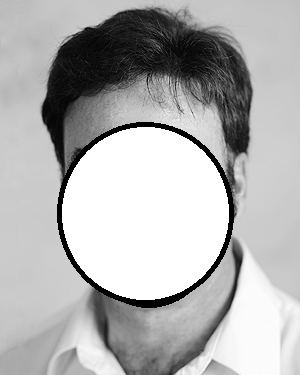
\includegraphics[width=1in,height=1.25in,clip,keepaspectratio]{author1.png}}]{First A. Author} received the B.S. and M.S. degrees in aerospace engineering from
the University of Virginia, Charlottesville, in 2001 and the Ph.D. degree in
mechanical engineering from Drexel University, Philadelphia, PA, in 2008.

From 2001 to 2004, he was a Research Assistant with the Princeton Plasma
Physics Laboratory. Since 2009, he has been an Assistant Professor with the
Mechanical Engineering Department, Texas A{\&}M University, College Station.
He is the author of three books, more than 150 articles, and more than 70
inventions. His research interests include high-pressure and high-density
nonthermal plasma discharge processes and applications, microscale plasma
discharges, discharges in liquids, spectroscopic diagnostics, plasma
propulsion, and innovation plasma applications. He is an Associate Editor of
the journal \emph{Earth, Moon, Planets}, and holds two patents.

Dr. Author was a recipient of the International Association of Geomagnetism
and Aeronomy Young Scientist Award for Excellence in 2008, and the IEEE
Electromagnetic Compatibility Society Best Symposium Paper Award in 2011.
\end{IEEEbiography}

\begin{IEEEbiography}[{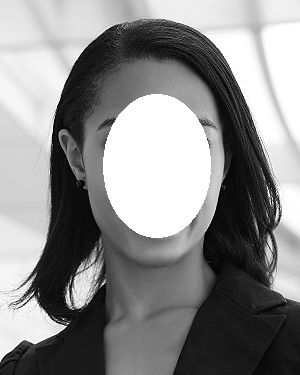
\includegraphics[width=1in,height=1.25in,clip,keepaspectratio]{author2.png}}]{Second B. Author} (M'76--SM'81--F'87) and all authors may include
biographies. Biographies are often not included in conference-related
papers. This author became a Member (M) of IEEE in 1976, a Senior
Member (SM) in 1981, and a Fellow (F) in 1987. The first paragraph may
contain a place and/or date of birth (list place, then date). Next,
the author's educational background is listed. The degrees should be
listed with type of degree in what field, which institution, city,
state, and country, and year the degree was earned. The author's major
field of study should be lower-cased.

The second paragraph uses the pronoun of the person (he or she) and not the
author's last name. It lists military and work experience, including summer
and fellowship jobs. Job titles are capitalized. The current job must have a
location; previous positions may be listed
without one. Information concerning previous publications may be included.
Try not to list more than three books or published articles. The format for
listing publishers of a book within the biography is: title of book
(publisher name, year) similar to a reference. Current and previous research
interests end the paragraph.

The third paragraph begins with the author's
title and last name (e.g., Dr.\ Smith, Prof.\ Jones, Mr.\ Kajor, Ms.\ Hunter).
List any memberships in professional societies other than the IEEE. Finally,
list any awards and work for IEEE committees and publications. If a
photograph is provided, it should be of good quality, and
professional-looking. Following are two examples of an author's biography.
\end{IEEEbiography}

\newpage

%If you do not have or do not want to include a photo, you can use IEEEbiographynophoto as shown below:

\begin{IEEEbiographynophoto}{Third C. Author, Jr.} (M'87) received the B.S. degree in mechanical
engineering from National Chung Cheng University, Chiayi, Taiwan, in 2004
and the M.S. degree in mechanical engineering from National Tsing Hua
University, Hsinchu, Taiwan, in 2006. He is currently pursuing the Ph.D.
degree in mechanical engineering at Texas A{\&}M University, College
Station, TX, USA.

From 2008 to 2009, he was a Research Assistant with the Institute of
Physics, Academia Sinica, Tapei, Taiwan. His research interest includes the
development of surface processing and biological/medical treatment
techniques using nonthermal atmospheric pressure plasmas, fundamental study
of plasma sources, and fabrication of micro- or nanostructured surfaces.

Mr. Author's awards and honors include the Frew Fellowship (Australian
Academy of Science), the I. I. Rabi Prize (APS), the European Frequency and
Time Forum Award, the Carl Zeiss Research Award, the William F. Meggers
Award and the Adolph Lomb Medal (OSA).
\end{IEEEbiographynophoto}

\end{document}